% Options for packages loaded elsewhere
\PassOptionsToPackage{unicode}{hyperref}
\PassOptionsToPackage{hyphens}{url}
%
\documentclass[
]{book}
\usepackage{amsmath,amssymb}
\usepackage{lmodern}
\usepackage{iftex}
\ifPDFTeX
  \usepackage[T1]{fontenc}
  \usepackage[utf8]{inputenc}
  \usepackage{textcomp} % provide euro and other symbols
\else % if luatex or xetex
  \usepackage{unicode-math}
  \defaultfontfeatures{Scale=MatchLowercase}
  \defaultfontfeatures[\rmfamily]{Ligatures=TeX,Scale=1}
\fi
% Use upquote if available, for straight quotes in verbatim environments
\IfFileExists{upquote.sty}{\usepackage{upquote}}{}
\IfFileExists{microtype.sty}{% use microtype if available
  \usepackage[]{microtype}
  \UseMicrotypeSet[protrusion]{basicmath} % disable protrusion for tt fonts
}{}
\makeatletter
\@ifundefined{KOMAClassName}{% if non-KOMA class
  \IfFileExists{parskip.sty}{%
    \usepackage{parskip}
  }{% else
    \setlength{\parindent}{0pt}
    \setlength{\parskip}{6pt plus 2pt minus 1pt}}
}{% if KOMA class
  \KOMAoptions{parskip=half}}
\makeatother
\usepackage{xcolor}
\IfFileExists{xurl.sty}{\usepackage{xurl}}{} % add URL line breaks if available
\IfFileExists{bookmark.sty}{\usepackage{bookmark}}{\usepackage{hyperref}}
\hypersetup{
  pdftitle={Photochemistry and Photophysics},
  pdfauthor={Fiona Dickinson},
  hidelinks,
  pdfcreator={LaTeX via pandoc}}
\urlstyle{same} % disable monospaced font for URLs
\usepackage{longtable,booktabs,array}
\usepackage{calc} % for calculating minipage widths
% Correct order of tables after \paragraph or \subparagraph
\usepackage{etoolbox}
\makeatletter
\patchcmd\longtable{\par}{\if@noskipsec\mbox{}\fi\par}{}{}
\makeatother
% Allow footnotes in longtable head/foot
\IfFileExists{footnotehyper.sty}{\usepackage{footnotehyper}}{\usepackage{footnote}}
\makesavenoteenv{longtable}
\usepackage{graphicx}
\makeatletter
\def\maxwidth{\ifdim\Gin@nat@width>\linewidth\linewidth\else\Gin@nat@width\fi}
\def\maxheight{\ifdim\Gin@nat@height>\textheight\textheight\else\Gin@nat@height\fi}
\makeatother
% Scale images if necessary, so that they will not overflow the page
% margins by default, and it is still possible to overwrite the defaults
% using explicit options in \includegraphics[width, height, ...]{}
\setkeys{Gin}{width=\maxwidth,height=\maxheight,keepaspectratio}
% Set default figure placement to htbp
\makeatletter
\def\fps@figure{htbp}
\makeatother
\setlength{\emergencystretch}{3em} % prevent overfull lines
\providecommand{\tightlist}{%
  \setlength{\itemsep}{0pt}\setlength{\parskip}{0pt}}
\setcounter{secnumdepth}{5}
\usepackage{booktabs}
\usepackage{amsthm}
\makeatletter
\def\thm@space@setup{%
  \thm@preskip=8pt plus 2pt minus 4pt
  \thm@postskip=\thm@preskip
}
\makeatother
\ifLuaTeX
  \usepackage{selnolig}  % disable illegal ligatures
\fi
\usepackage[]{natbib}
\bibliographystyle{apalike}

\title{Photochemistry and Photophysics}
\author{Fiona Dickinson}
\date{2022-07-04}

\begin{document}
\maketitle

{
\setcounter{tocdepth}{1}
\tableofcontents
}
\hypertarget{welcome}{%
\chapter*{Welcome}\label{welcome}}
\addcontentsline{toc}{chapter}{Welcome}

The notes have been prepared in a package called BookDown for RStudio so that the equations are accessible to screen readers. However, by providing the notes as a .html webpage I have also been able to embed short concept bite videos to further describe some of the topics. Further you can access the notes in a format that suits you:

\begin{itemize}
\tightlist
\item
  download the notes (top bar on the screen) (either pdf or epub) to view offline (videos will not download).
\item
  or change the way this document appears for ease of reading (A button in toolbar), changing the font, font size and background colour.
\end{itemize}

The document is also searchable (magnifying glass in header bar) and you can access or remove the navigation list by clicking on the four horizontal lines in the header bar.

This is a relatively new format of the document and is easily editable, therefore if you do find any typing errors, areas with lack of clarity, or other errors please let me know. I will update the document accordingly and update the version history below. If there are any major changes I will inform you as a class. I can and will also address areas where you feel there isn't enough detail, just use the same form below.

\hypertarget{sec:AddnRes}{%
\section{Additional Resources}\label{sec:AddnRes}}

Whilst this resource is designed to stand alone, you will find it beneficial to read around the subject or else listen to the concept bites. I refer to the book by Wardle frequently and you have access to it digitally \emph{via} the library, although there are a number of excellent photochemistry textbooks which I've listed below.

Whilst this is designed to be independent study it does not mean that you are alone in your learning. Please feel free to contact me for help or feedback (using Teams or email) and I can also help facilitate the formation of study groups. The value of peer interactions when learning cannot be overstated, find yourself a study buddy and help each other with your misconceptions and difficulties.

\hypertarget{reading-list}{%
\subsection*{Reading list}\label{reading-list}}
\addcontentsline{toc}{subsection}{Reading list}

Resources marked with a * have online access.

\begin{itemize}
\item
  *\href{https://bibliu.com/app/\#/view/books/9780198558866/epub/html/toc.html}{Photochemistry}, Carol E. Wayne \& Richard P. Wayne. Oxford: OUP, 1996. Oxford Science Publications. ISBN 0198558864
\item
  \href{https://bath-ac-primo.hosted.exlibrisgroup.com/primo-explore/fulldisplay?docid=44BAT_ALMA_DS2131580390002761\&context=L\&vid=44BAT_VU1\&lang=en_US\&search_scope=CSCOP_44BAT_DEEP\&adaptor=Local\%20Search\%20Engine\&tab=local\&query=any,contains,photochemistry\&sortby=rank\&facet=rtype,include,books\&offset=0\&pcAvailability=false}{Photochemistry} Calvert, J G., and J N. Pitts. Photochemistry.
\item
  *\href{https://ebookcentral.proquest.com/lib/bath/detail.action?docID=470772\&pq-origsite=primo}{Principles and Applications of Photochemistry} Brian Wardle, Wiley, 2009. ISBN 0470014938
\item
  *\href{https://ebookcentral.proquest.com/lib/bath/detail.action?pq-origsite=primo\&docID=1662200}{Photochemistry and Photophysics: Concepts, Research, Applications} Balzani, Vincenzo, Paola Ceroni, and Alberto Juris. P. Weinheim, Germany: Wiley-VCH, 2014.
\item
  \href{https://bath-ac-primo.hosted.exlibrisgroup.com/primo-explore/fulldisplay?docid=44BAT_ALMA_DS2129513080002761\&context=L\&vid=44BAT_VU1\&lang=en_US\&search_scope=CSCOP_44BAT_DEEP\&adaptor=Local\%20Search\%20Engine\&tab=local\&query=any,contains,\%22modern\%20molecular\%20photochemistry\%22\%20turro\&offset=0\&pcAvailability=false}{Modern Molecular Photochemistry of Organic Molecules} Turro, N.J., Ramamurthy, V., and Scaiano, J. C. Modern Molecular Photochemistry of Organic Molecules. Sausalito, Calif.: U Science, 2010.
\item
  *\href{https://link.springer.com/book/10.1007/978-0-387-46312-4}{Principles of Fluorescence Spectroscopy (3rd Edition)} Joseph R. Lakowicz, Springer, 2006. ISBN 0387312781
\item
  *\href{https://bath-ac-primo.hosted.exlibrisgroup.com/primo-explore/fulldisplay?docid=44BAT_ALMA_DS2129552010002761\&context=L\&vid=44BAT_VU1\&lang=en_US\&search_scope=CSCOP_44BAT_DEEP\&adaptor=Local\%20Search\%20Engine\&tab=local\&query=any,contains,principles\%20of\%20molecular\%20photochemistry\%20ramamurthy\&offset=0\&pcAvailability=false}{Principles of Molecular Photochemistry: An Introduction}, Nicholas J.Turro,V. Ramamurthy, J.C. Scaiano, University Science Books, ISBN 1891389573
\end{itemize}

\hypertarget{report-errors}{%
\section{Report errors}\label{report-errors}}

If you spot any errors or areas of lack of clarity, please message me in Teams or preferably report on the error log below:

Loading\ldots{}

\hypertarget{version-history}{%
\section*{Version history}\label{version-history}}
\addcontentsline{toc}{section}{Version history}

Semi-major update for clarity and to fix issues with pdf not showing symbols. Begun 28 June 2022.

Trying to fix legacy errors ready for the year 13th October 2021.

Updated for pdf but introduced errors with sub and superscripts in figure captions 9th October 2020.

Updated with learning outcomes for each chapter and updated content in chapter 6. 8th September 2020.

The initial commit of this book is dated 6th September 2020.

\hypertarget{ch:Intro}{%
\chapter{Introduction to Photochemistry \& Photophysics}\label{ch:Intro}}

Let us open with some context on this course.

Photochemistry is, by definition from IUPAC, `the branch of chemistry concerned with the chemical effects of light'\footnote{IUPAC Goldbook, \url{http://goldbook.iupac.org/terms/view/P04588} (accessed July 2020).}. However, in this course we are going to focus on and examine some of the fundamental \textbf{photophysics} of system before finally introducing chemical reactions involving light. Photophysics is closely related to what you have previously studied in your first and second years, in that it is a study of the processes of absorption and emission of light and the kinetics of these processes. We will also draw upon your previous studies of quantum mechanics as wavefunctions are vital in our understanding of photophysical processes.

Light is the very reason why there is life on earth, the outstanding beauty of processes such as photosynthesis or vision speak to the power of this branch of chemistry. Photochemistry offers a way for us to `cheat' traditional chemical reactions, in that we no longer need thermal energy to get over an activation barrier, instead we use the energy of a photon. It is only by understanding how we can best utilise the bounteous resource of the sun's light that we as a species can hope to to have a long and fruitful future on this planet.

It is just over 100 years since quantum theory revolutionised our understanding of matter and light, 125 years since the discovery of the electron, but in that time we have achieved wonderful things, things that have revolutionised the way we live. From lasers in cd and blue ray players to their use in scanning bar codes, glow sticks (fun at festivals, essential in emergencies), or more prosaic uses such as sun creams, self cleaning windows or display technology (where would we be without the phones in our pockets?). In this course you will learn about a range of photophysical and photochemical processes that underpin our modern lives and also learn about some of the current challenges and interests in the field.

\textbf{Spectroscopy}

\begin{itemize}
\tightlist
\item
  techniques
\end{itemize}

\textbf{Photochemistry}

\begin{itemize}
\tightlist
\item
  reactions
\item
  molecular structure
\end{itemize}

\textbf{Photophysics}

\begin{itemize}
\tightlist
\item
  kinetics
\item
  thermodynamics
\item
  quantum mechanics
\end{itemize}

\textbf{Photophysical processes}

*transitions which convert between excited states or between an excited state and a ground state of a molecule

\textbf{Photochemical processes}

*reactions or rearrangements which occur as a consequence of excitation from the ground state

\hypertarget{assumed-background-knowledge}{%
\section{Assumed background knowledge}\label{assumed-background-knowledge}}

The course relies heavily on first and second year kinetics concepts as well as building on the quantum mechanics from second year and some of the spectroscopy you did in first year. Whilst I have done my best to ensure that there is a minimum of non-physical chemistry content required to get the most out of this course if I want to talk about molecules some very basic knowledge from both organic and inorganic chemistry, much of which will at least have been mentioned at `A'-level or IB.

I will talk a lot about \(\sigma\) and \(\pi\) bonding, but this has been covered in quantum mechanics, a double bond has one \(\sigma\) and one \(\pi\) bond. I will also talk about shape and structure, a carbon with only \(\sigma\) bonds is 3 dimensional and tetrahedral, a carbon with 3 \(\sigma\) and 1 \(\pi\) bond is trigonal planar, and one with 2 \(\sigma\) and 2 \(\pi\) bonds is linear.

However we need to think about the fact that a molecular orbital exists over a hole molecule. If we reduce bond order overall we change the shape of the molecule. This will be discussed in the absorption (Chapter \ref{ch:Abs}) section of this course.

If you need more help on structure, bonding or metal complexes Chemistry\textsuperscript{3} is an excellent book to start with, or please ask for help.

\begin{figure}

{\centering 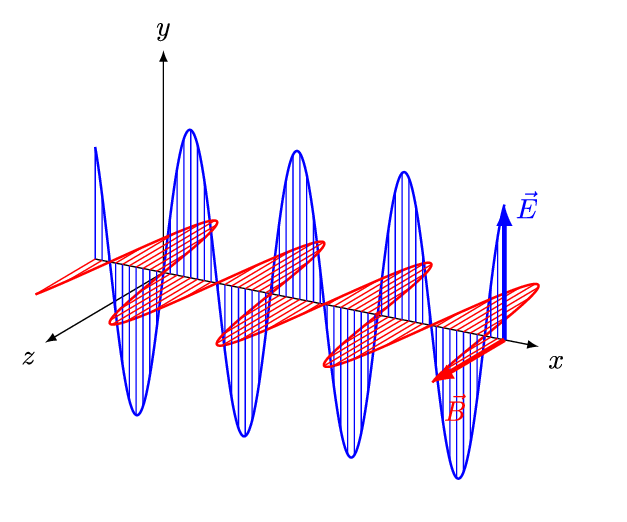
\includegraphics[width=0.6\linewidth]{images/EM-Wave} 

}

\caption{Light as a wave is made up of orthogonal oscillating electric and magnetic fields. From: [And1mu](https://upload.wikimedia.org/wikipedia/commons/9/99/EM-Wave.gif) / [CC BY-SA](https://creativecommons.org/licenses/by-sa/4.0)}\label{fig:EMWave}
\end{figure}

\hypertarget{sec:Light}{%
\section{Light}\label{sec:Light}}

As you've already learnt light exhibits properties that has both a wave like and particle like nature, and our understanding of light was one of the fundamental pieces that lead towards the quantum theory of the atom. Newton had shown that light from the sun is comprised of a spectrum of colours, we now know that that spectrum goes beyond what we can see with our eyes.

\begin{figure}
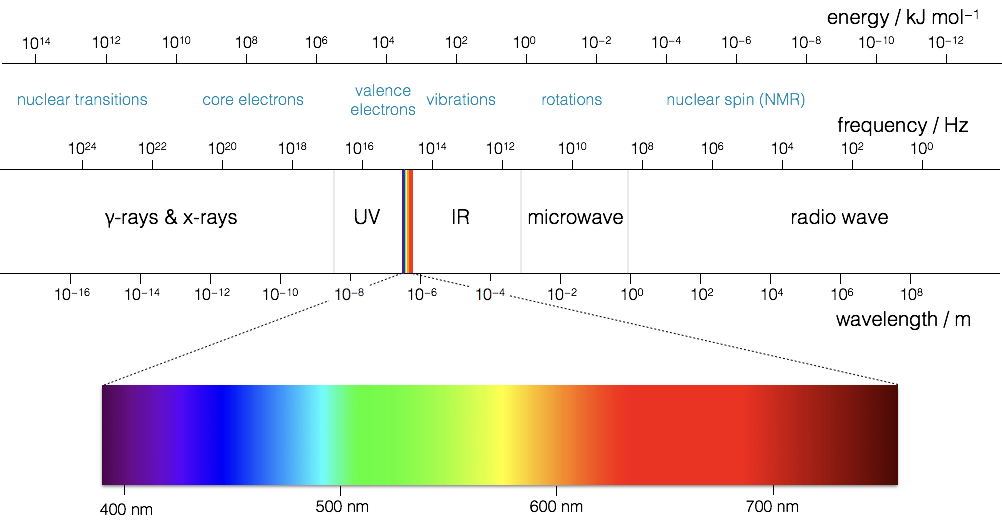
\includegraphics[width=1\linewidth]{images/EMspectrumspectroscopy} \caption{The electromagnetic spectrum of light, frequency and energy are equivalent, so high frequency waves have high energy photons}\label{fig:EMspect}
\end{figure}

In your studies you have already seen how large amounts of the electromagnetic spectrum is used for different spectroscopic techniques, making use of the quantised transitions within molecules. For example, infra-red light has the same energy as the vibrational transitions within molecules. In photochemistry, we are specifically interested in the visible and near UV part of the EM spectrum as photons with this energy promote transitions for the valance electrons in the molecules we are interested in.

It is important never to forget the wave particle duality of light, however for much of photochemistry and photophysics it is perhaps simpler to consider the light as a stream of incident photons, whilst there are classical (wave) models to thing of processes like absorption and emission this set of notes will usually defer to an entirely particle model of absportion or emission of a photon.

\hypertarget{feedback-on-this-resource}{%
\section*{Feedback on this resource}\label{feedback-on-this-resource}}
\addcontentsline{toc}{section}{Feedback on this resource}

Loading\ldots{}

\hypertarget{formative-questions-subsecintroqs}{%
\section{Formative questions \{subsec:introqs\}}\label{formative-questions-subsecintroqs}}

\hypertarget{ch:Abs}{%
\chapter{Absorption of light}\label{ch:Abs}}

\hypertarget{sec:AbsLOs}{%
\subsection{Learning Objectives}\label{sec:AbsLOs}}

At the end of this section you should be able to:

\begin{itemize}
\tightlist
\item
  Appreciate changes in molecular geometry brought about by light absorption
\item
  Use the Beer Lambert Law to calculate light absorption
\item
  Discuss electronic transitions in terms of Morse energy curves
\item
  Explain the Franck Condon principle and Franck Condon factors
\item
  List selection rules for excitation of a photon and describe factors which affect the molar extinction coefficient
\item
  Explain some of the factors which affect absorption
\end{itemize}

There is a Concept Bite video in Section \ref{sec:before1} which summarises much of this content.

\hypertarget{sec:AbsIntro}{%
\section{Introduction}\label{sec:AbsIntro}}

As you have previously learnt energy levels are quantised, in other words atoms and molecules can only have defined amounts of energy. Different transitions (electronic, vibrational, rotational) in atoms and molecules use different characteristic portions of the electromagnetic spectra, Figure \ref{fig:EMspect}.

When you saw atomic absorption and emission spectra the lines were very sharp, or in other words the absorption bands are very narrow as shown for the hydrogen absorption and emission spectra (figure \ref{fig:HAbsEm}).This isn't the case with molecular absorption spectra, particularly those in solution where absorption bands are typically hundreds of nanometers broad a typical organic fluorophor is shown in figure \ref{fig:RhoAbsEm}.The broad nature of the bands in molecular systems is a product of many individual factors including solvation, vibrational \& rotational factors and non minimised structural configurations.

\begin{figure}

{\centering 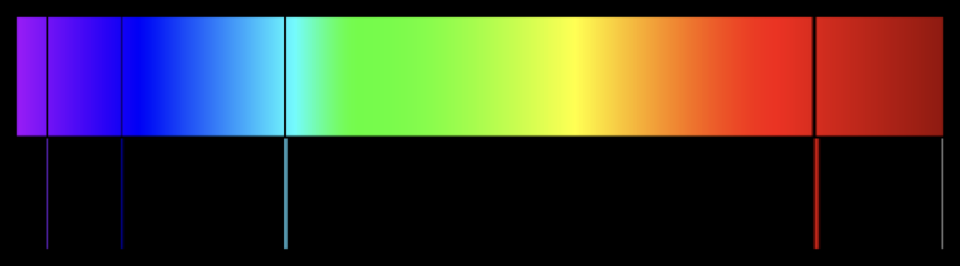
\includegraphics[width=0.7\linewidth]{images/HAbsEm} 

}

\caption{The absorption (top) and emission (bottom) spectra of hydrogen showing the very narrow band features, [image](http://montessorimuddle.org/2012/02/01/emission-spectra-how-atoms-emit-and-absorb-light/) adapted from [Adrignola](https://commons.wikimedia.org/wiki/User:Adrignola) licensed under CC BY 2.0}\label{fig:HAbsEm}
\end{figure}

\begin{figure}

{\centering 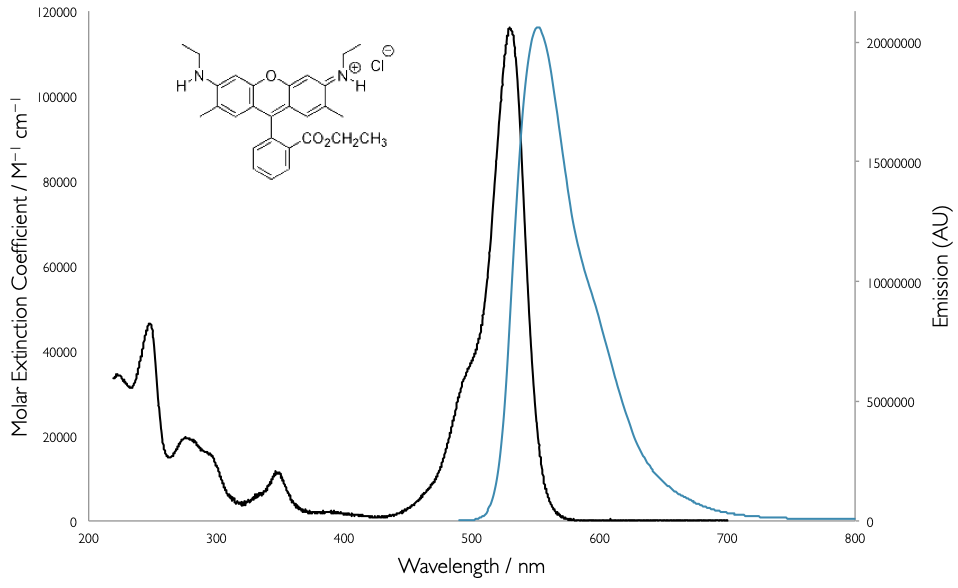
\includegraphics[width=0.6\linewidth]{images/Rhodamine6GAbsEm} 

}

\caption{The absorption (black) and emission (teal) spectra of Rhodamine 6G in ethanol. The emission spectra was recorded with an excitation wavelength of 480 nm and a bandwidth of 4.25 nm [Adapted from [OMLC](https://omlc.org/spectra/PhotochemCAD/html/083.html), [2nd July 2014]]}\label{fig:RhoAbsEm}
\end{figure}

\hypertarget{sec:BeerLambert}{%
\section{Beer-Lambert Law}\label{sec:BeerLambert}}

The empirical equation (equation \eqref{eq:BeerLambert}, figure \ref{fig:BeerLambert}) implies that the probability of a photon being absorbed at any point is the same (much like first order kinetics), and the amount of the total absorption depends upon the the concentration of the sample, c, and the `path length', l.

The amount of absorbance, A, is dependent upon the wavelength of the incident light, and the constant of proportionality, \(\varepsilon\) (here called the molar extinction coefficient), is consequently also wavelength dependent.
\begin{equation}
\log \frac{I_0}{I}=A=\varepsilon cl
\label{eq:BeerLambert}
\end{equation}

The wavelength of a particular value of the molar exctinction coefficient is often represted as a subscript, \(\varepsilon _\lambda\)

\begin{figure}

{\centering 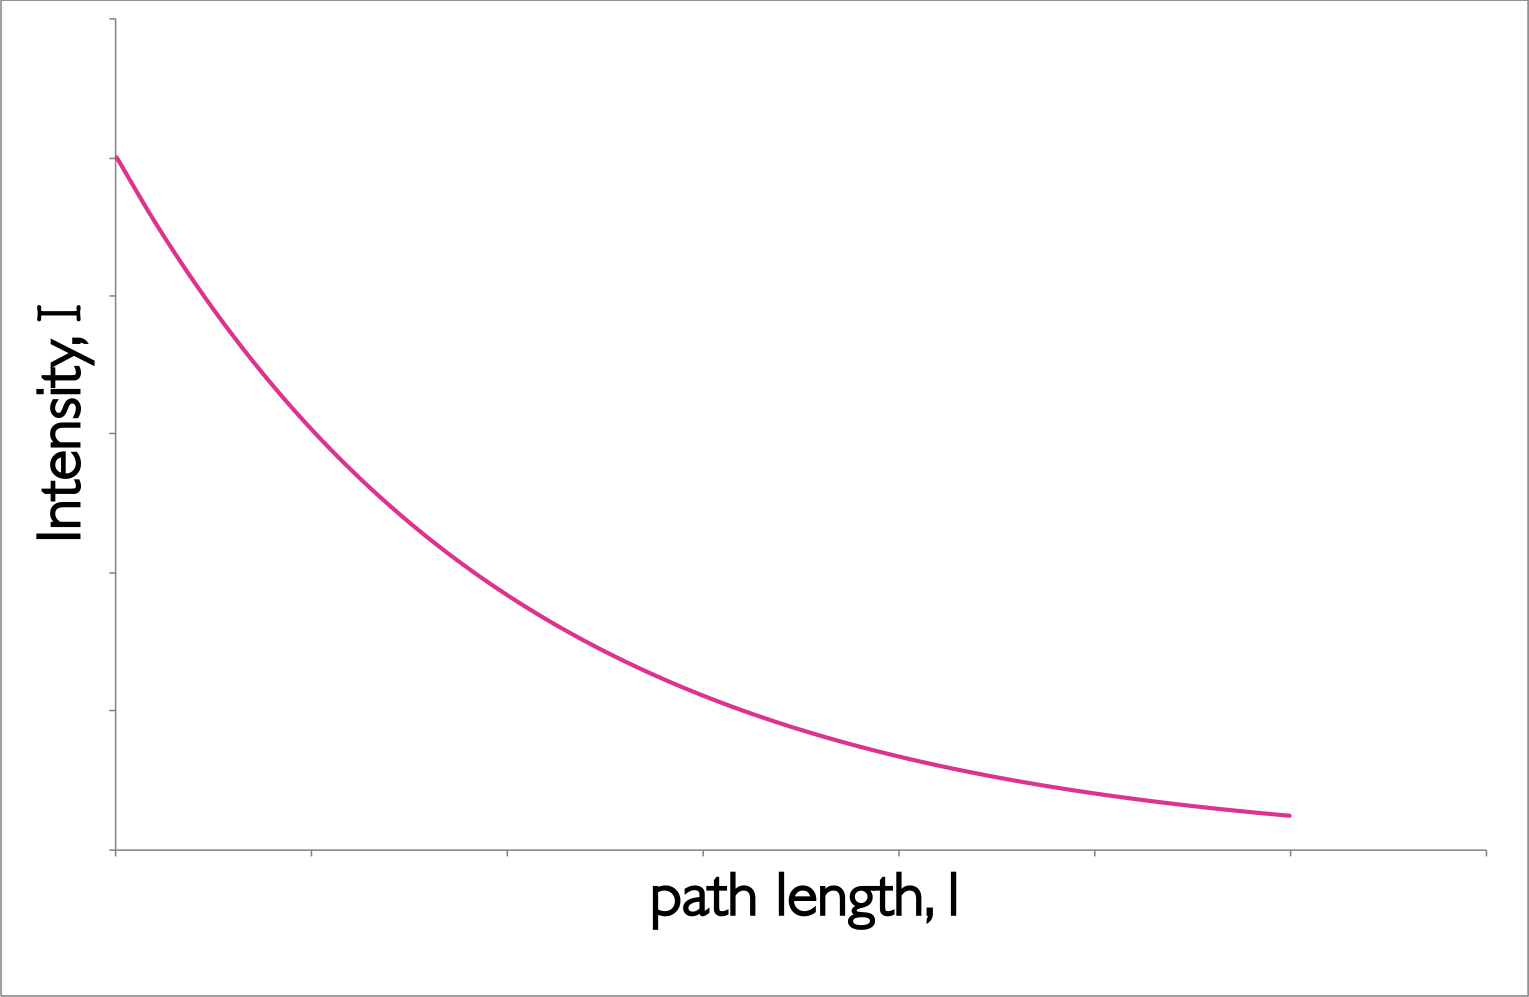
\includegraphics[width=0.5\linewidth]{images/BeerLambert} 

}

\caption{The decay of intensity of monochromatic incident light through a uniformly absorbing medium. The decay follows an exponential pattern as elucidated in the Beer-Lambert equation.}\label{fig:BeerLambert}
\end{figure}

The Beer-Lambert law makes a number of assumptions, and this exponential decay of the intensity of light is an important factor.When using the Beer-Lambert law you consider the intensity of the incident radiation, there is an assumption that the intensity of the radiation reaching each part of the sample does not deviate much from this. Hence high absorbing samples tend to show strong deviation from the Beer-Lambert's linear relationship.

The Beer-Lambert law also has to make a number of other `reasonable' considerations:

\begin{itemize}
\tightlist
\item
  The solutions is well mixed, and absorbers are homogeneously distributed in solution.
\item
  The absorbers do not scatter radiation (all particles will Rayleigh and Raman scatter but this is normally considerably less intense than absorption). Consequently solutions should be optically transparent as optically opaque solutions (such as colloidal solutions) have considerably stronger scattering.
\item
  The absorbers acts independently of each other, this means solutions need to be at a reasonably low concentration (typically less than 0.01 M, or maybe even less depending on the species) so as to avoid electrostatic or \(\pi\) stacking interactions between the chromophores.This is in part important because light is only absorbed when the polarisation of the light is aligned with the transition dipole moment.
\item
  The incident radiation is collimated, and each photon should pass through the same path length.
\item
  The sample holder (cuvette) is optically `pure' such that reflections are avoided (linked to the assumption above).
\item
  The incident radiation is monochromatic, or at the very least has a band width more narrow than the band width of the absorbing transition (this is usually not an issue for molecular systems as bandwidths are usually 10s or more of nm wide, but for atomic or ion spectroscopy where bandwidths are \textless0.02 nm this is a factor which must be carefully considered.
\item
  The incident radiation does not noticeably affect the concentration of the ground state, in other words the amount of excited states generated must be kept small as when we are talking about the absorption of a chromophore the concentration of that chromophore that appears in the Beer-Lambert equation is the ground state concentration.
\item
  There is no measurable emission from the sample.
\end{itemize}

However, this empirical relationship can be examined in a deeper way.

\hypertarget{sec:Einstein}{%
\section{Einstein Absorption and Emission Factors}\label{sec:Einstein}}

If we consider the simplest case of absorption, a molecule absorbs an incident photon and this process creates an excited state within the molecule, figure \ref{fig:AbsStimEm}a.

\begin{figure}

{\centering 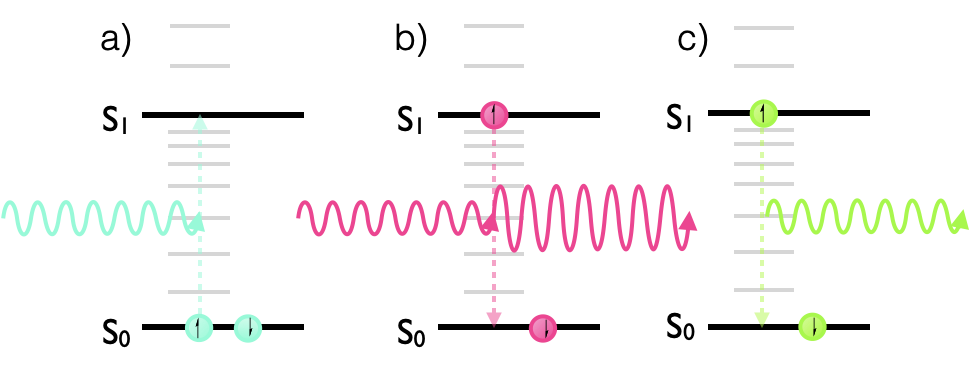
\includegraphics[width=0.7\linewidth]{images/AbsStimEm} 

}

\caption{The allowed transitions within a photonic system: a) stimulated absorption, b) stimulated emission, c) spontaneous emission.}\label{fig:AbsStimEm}
\end{figure}

\begin{equation}
A+ h \nu \longrightarrow A^\ast \hspace{3cm} k_A \hspace{1cm} \textrm{Absorption}
\label{eq:Abs}
\end{equation}

From the empirical Beer-Lambert relationship we can say that the `amount' of absorption is related to the molar `extinction coefficient', but how does this relate to our quantum mechanical understanding of molecules?

Some simple logical deduction can be used to explain some of the concepts of quantum mechanics.
Einstein proposed that the rate of `stimulated absorption' of a photon is related to the strength of the oscillating electromagnetic field (or the flux of incident photons, in a quantised model). Logically the greater the intensity of the electromagnetic field, p, the greater the rate of the stimulated absorption, \(\omega\). In fact:

\begin{equation}
\omega \longrightarrow B p \hspace{3cm} \textrm{rate of stimulated absorption}
\label{eq:StimAbs}
\end{equation}

In equation \eqref{eq:StimAbs} the constant of proportionality, \(B\), is called the Einstein coefficient of stimulated absorption; the greater the value of \(B\) the higher the rate of absorption of light, so consequently it plays a similar role to the molar extinction coefficient, \(\varepsilon\), in the Beer-Lambert law (equation \eqref{eq:BeerLambert}).

Einstein also suggested that the presence of an electromagnetic field could induce `stimulated emission', figure \ref{fig:AbsStimEm}b, from molecules with electrons in an excited state; this is an incredibly important process and is the basis of the laser. It requires the presence of an appropriate frequency of light in order to induce the transition from the excited state to the ground state and emission of a photon. In this case (as is often the case with atomic and molecular transitions) it is definitely easier to think of this process as photon rather than wave based.

\begin{equation}
A^\ast + h \nu \longrightarrow A + 2h \nu \hspace{3cm} k_{st} \hspace{1cm}\textrm{stimulated emission}
\label{eq:StimEm}
\end{equation}

Radiation of the same frequency (energy) as the transition is required to induced stimulated emission of light. The rate of stimulated emission from the excited state, ω', is again directly proportional to the strength of the electromagnetic field (flux of photons):

\begin{equation}
\omega ' \longrightarrow B' p \hspace{3cm} \textrm{rate of stimulated emission}
\label{eq:rateStimEm}
\end{equation}

where \(B’\) is the Einstein coefficient of stimulated emission.

The final case recognised by Einstein is the example of spontaneous emission, figure \ref{fig:AbsStimEm}c.~

\begin{equation}
A^\ast \longrightarrow A + h \nu \hspace{3cm} k_{sp} \hspace{1cm}\textrm{spontaneous emission}
\label{eq:SponEm}
\end{equation}

Deactivation of an excited state by emission of a photon without any dependence upon the strength of any electromagnetic field (indeed the simplest case is to consider the emission with no electromagnetic field):

\begin{equation}
\omega ' \longrightarrow A \hspace{3cm} \textrm{rate of spontaneous emission}
\label{eq:rateStimEm}
\end{equation}

where \(A\) is the Einstein coefficient of spontaneous emission.

In reality, emission is always a combination of both the stimulated and spontaneous emission processes, and so we can combine the equations to give a rate of deactivation of the excited state.

\begin{equation}
\omega ' \longrightarrow A + B'p \hspace{3cm} \textrm{overall rate of emission}
\label{eq:rateEm}
\end{equation}

The overall rate of each of these processes depends upon the number of molecules in the system. If we look simply at a Boltzmann distribution at room temperature almost all of the molecules are going to be in the ground state, as the spacing of electronic energy levels is significantly higher than the thermal energy of the system. If we considered that the `rate' is first order in `population of state' then, taking into account the populations of the ground state, \(N\), and excited state \(N’\), we can see:

\begin{equation}
W  \longrightarrow NBp \hspace{3cm} \textrm{overall combined rate of stimulated absorption}
\label{eq:totrateAbs}
\end{equation}

\begin{equation}
W ' \longrightarrow N'(A + B'p) \hspace{3cm} \textrm{overall combined rate of emission}
\label{eq:totrateEm}
\end{equation}

where \(W\) \& \(W’\) are the total rate of absorption of photons and emission of photons respectively.
It can be shown\footnote{see Atkins' Physical Chemistry, Spectroscopy chapter} that the constants \(B\) \& \(B’\) are the same for an atomic system, with the rate of of stimulated absorption and stimulated emission only varying due to the relative populations of the ground and excited state. In molecular systems, we shall see that the excited state `relaxes' and so has a different energy so Einstein's model has to be developed further, but the principles of stimulated absorption, spontaneous emission and stimulated emission are all valid whether an atomic or molecular system.

\hypertarget{sec:MOs}{%
\section{Molecular orbitals, HOMO \& LUMO}\label{sec:MOs}}

Ultimately, the absorption (and emission of a photon) which can be modelled empirically, as in the Beer-Lambert lawn, is actually a property of the quantum mechanics of the system as indicated by the models of absorption and emission of photons by Einstein.

If we think about the size of an atom or molecule (atoms are 100s of pm, molecules frequently less than 1 nm) they are considerably smaller than the wavelength of light required for electronic transitions, so it is often easier to think of an entirely photonic model of light.

If we considered the atom or molecules to be formed of a cloud of electrons bathed in the electromagnetic field, the electron density is attracted to the the positive side of the field, and the positively charged nucleus to the negative side. However, electrons are much lighter (about 1/1760 the mass of a a proton) and so it is the lighter electrons that `feel' the most effect. As the electric field oscillates it pushes and pulls the electrons within the molecule.

This transition is called an electric-dipole transition since it either creates (absorption) or destroys (emission) an oscillating electric dipole in the atom or molecule.The transition dipole moment, \(\mu_i\), arises from the charge displacement during the transition. The magnitude of this transition dipole moment depends upon the distance the net electronic charge is moved from the ground state average position. This transition dipole is entirely independent of any permanent dipole moment within the molecule.

Figure \ref{fig:Butadiene} shows the valence molecular orbitals of butadiene, showing the discrete energy levels in the system, absorption of a photon allows an electron to be excited from the highest occupied molecular orbital (HOMO) to any excited state.

Upon excitation of an electron there is a mixing of the molecular orbitals of the fully and partially occupied molecular orbitals, in the case of butadiene excitation of an electron from the HOMO to the LUMO (lowest unoccupied molecular orbital), giving the central C-C bond some double bond character, limiting rotation and leading to a structural change of the excited state.

\begin{figure}

{\centering 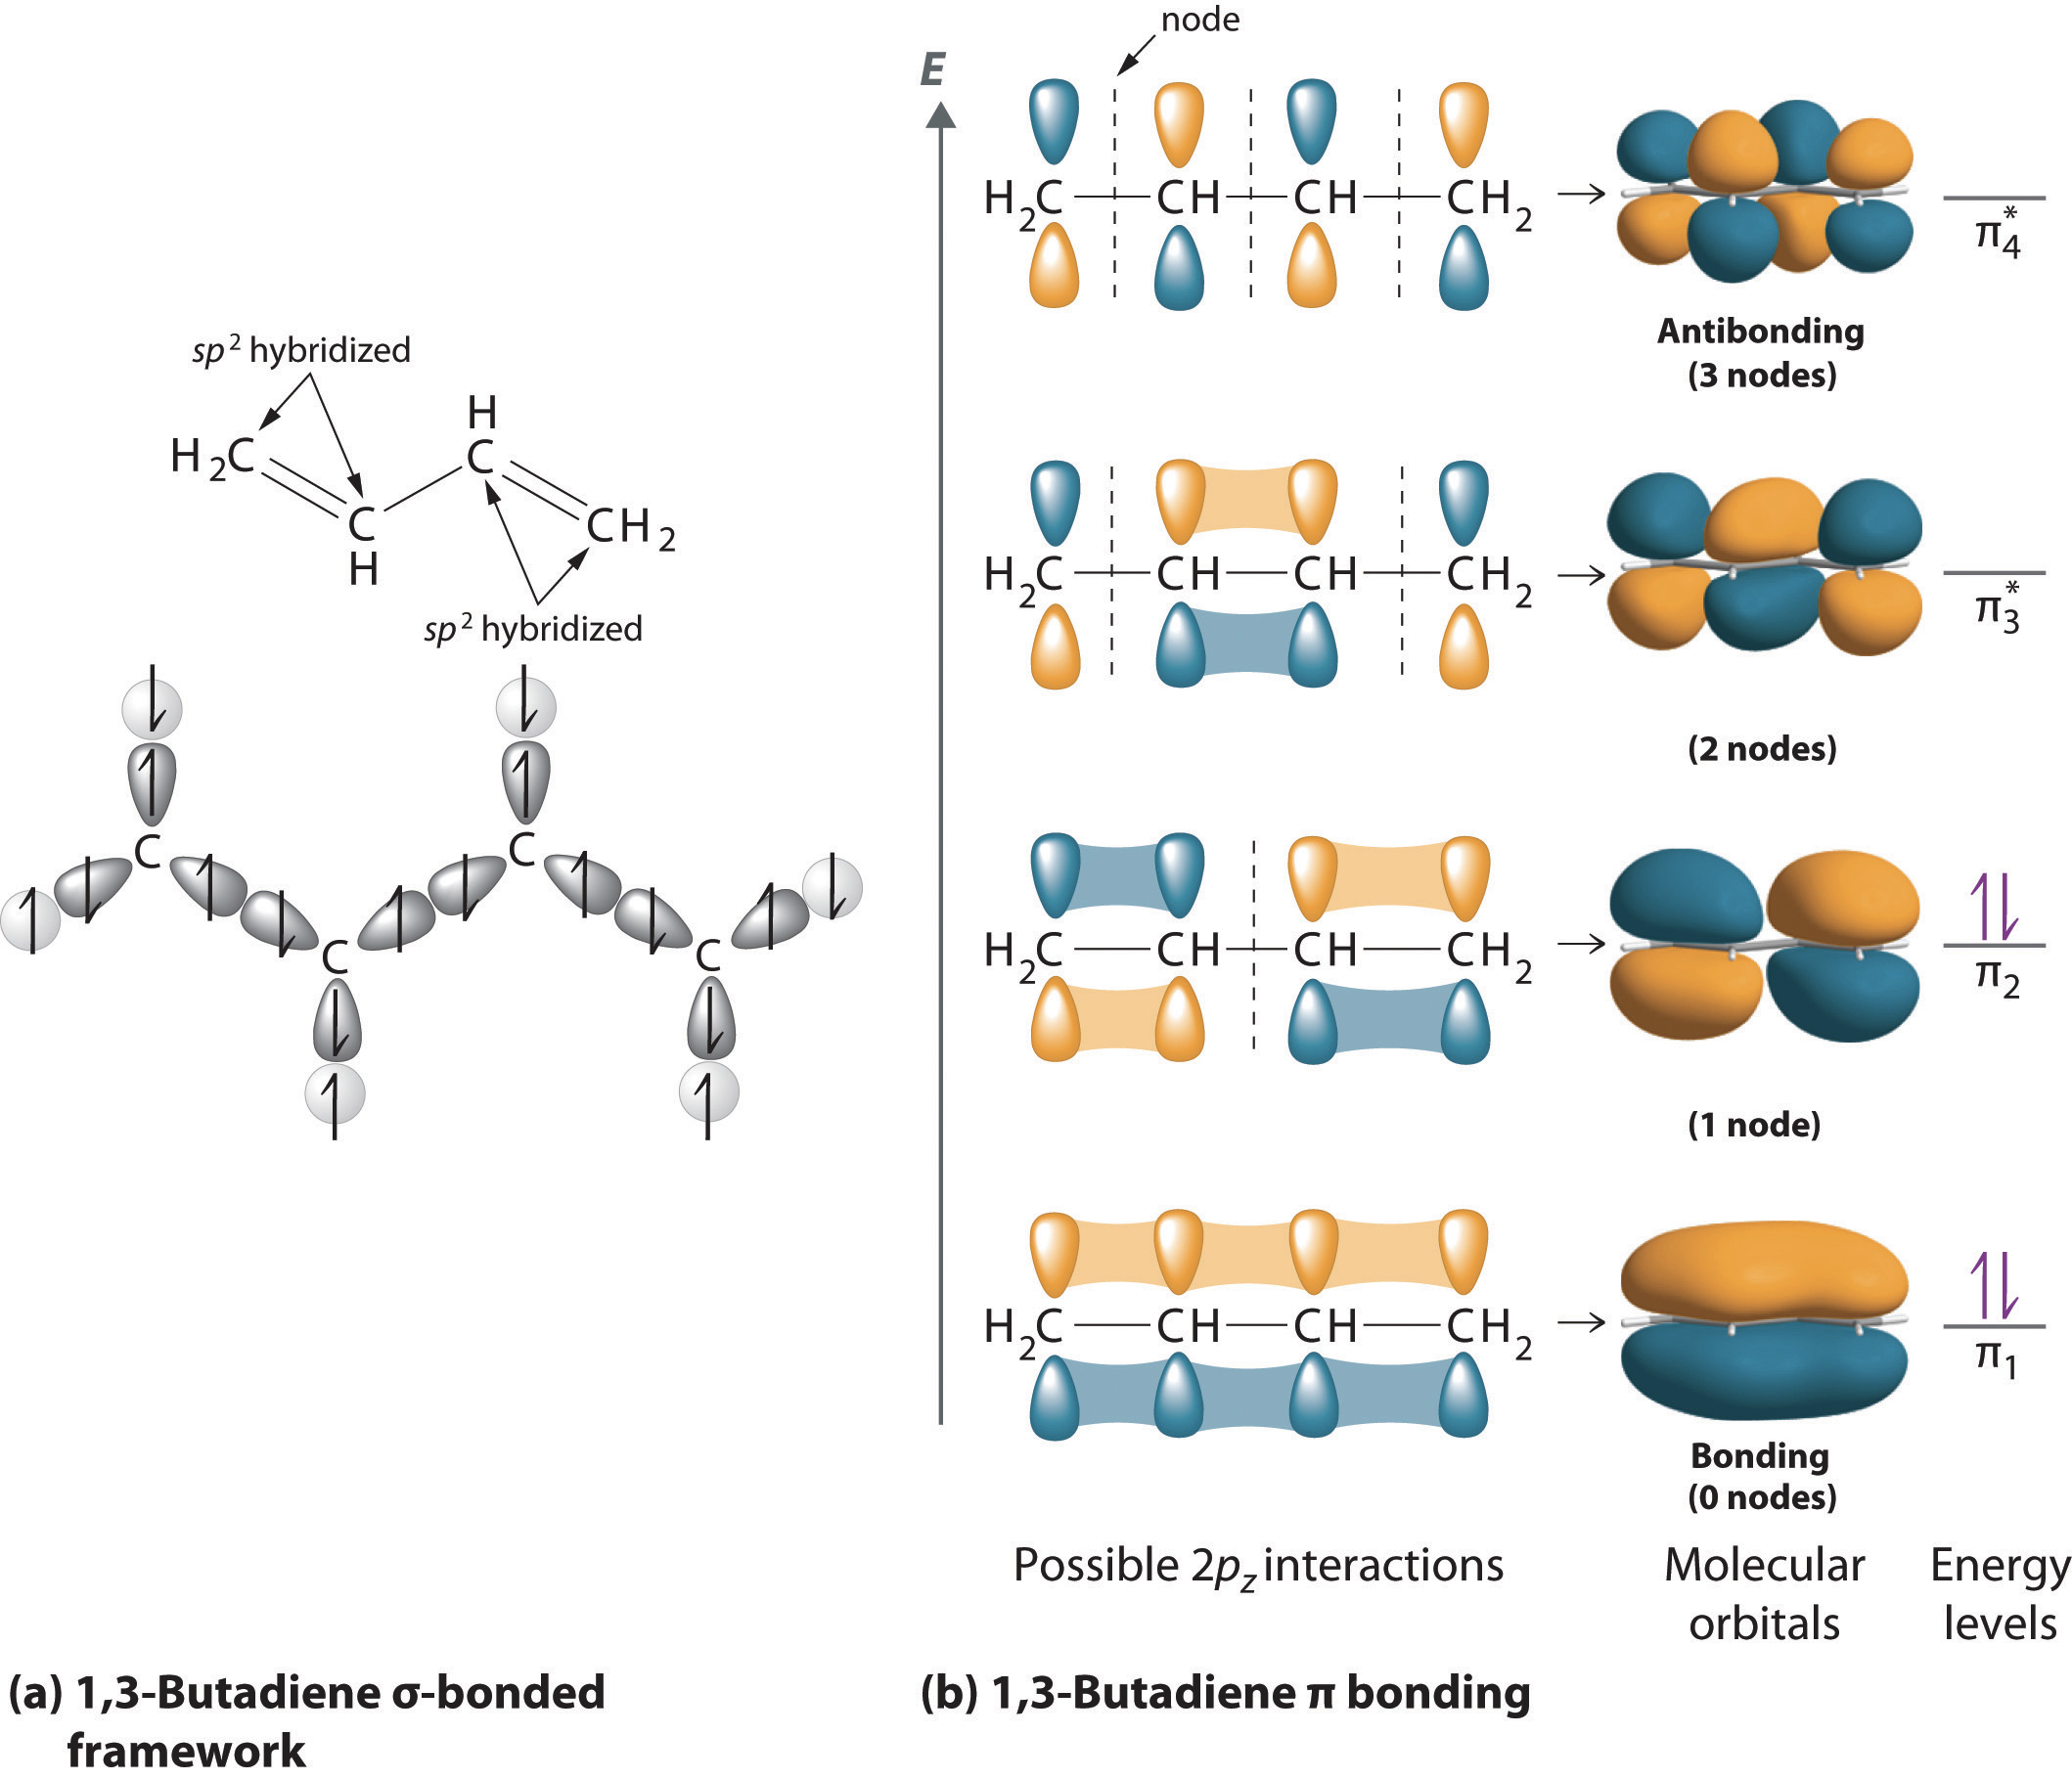
\includegraphics[width=0.7\linewidth]{images/Butadiene} 

}

\caption{MO diagram of butadiene, each carbon atom is assumed to be sp2 hybridised, with linear combination of the 2pz orbitals. As the energy of the levels increases so does the number of nodes. The lowest two energy levels are fully occupied in the ground state, upon absorption of a photon an electron is promoted to one of the anti-bonding orbitals allowing rotation around the double bonds, and giving the centre single bond some double bond character. MO diagram of butadiene (https://2012books.lardbucket.org/books/principles-of-general-chemistry-v1.0m/s13-04-polyatomic-systems-with-multip.html). From by Averill and Eldredge, Principles of General Chemistry licensed under CC BY 2.0. Sept 14.}\label{fig:Butadiene}
\end{figure}

In simple organic molecules we only really need to consider \(\pi\) and \(\pi^\ast\) and \(n\) (non-bonding) molecular orbitals as the energy difference between \(\sigma\) and \(\sigma^\ast\) orbitals are comparatively very large.

The process of absorption of a photon is very fast (\textasciitilde1 fs) (compared with the timescales of vibrations in molecule (\textasciitilde10 ps)), this is the basis of the Franck-Condon principle. Consequently when absorption (and emission) processes are sketched, as in figure \ref{fig:FrankCondon}, absorption and emission can be indicated by vertical transitions.

The `strength' of the absorption transition, which relates to the extinction coefficient in the Beer-Lambert law, and the Einstein \(B\) coefficient is in fact a measure of the `overlap integral' of the wave functions of the ground and excited states.
It becomes more obvious why the Einstein \(B\) and \(B’\) factors are only the same in atomic systems, since in the usual `lifetime' of the excited state of molecular systems there is plenty of opportunity for the molecule to undergo structural rearrangement or loose energy if excited into one of the vibrationally excited bands.

\begin{figure}

{\centering 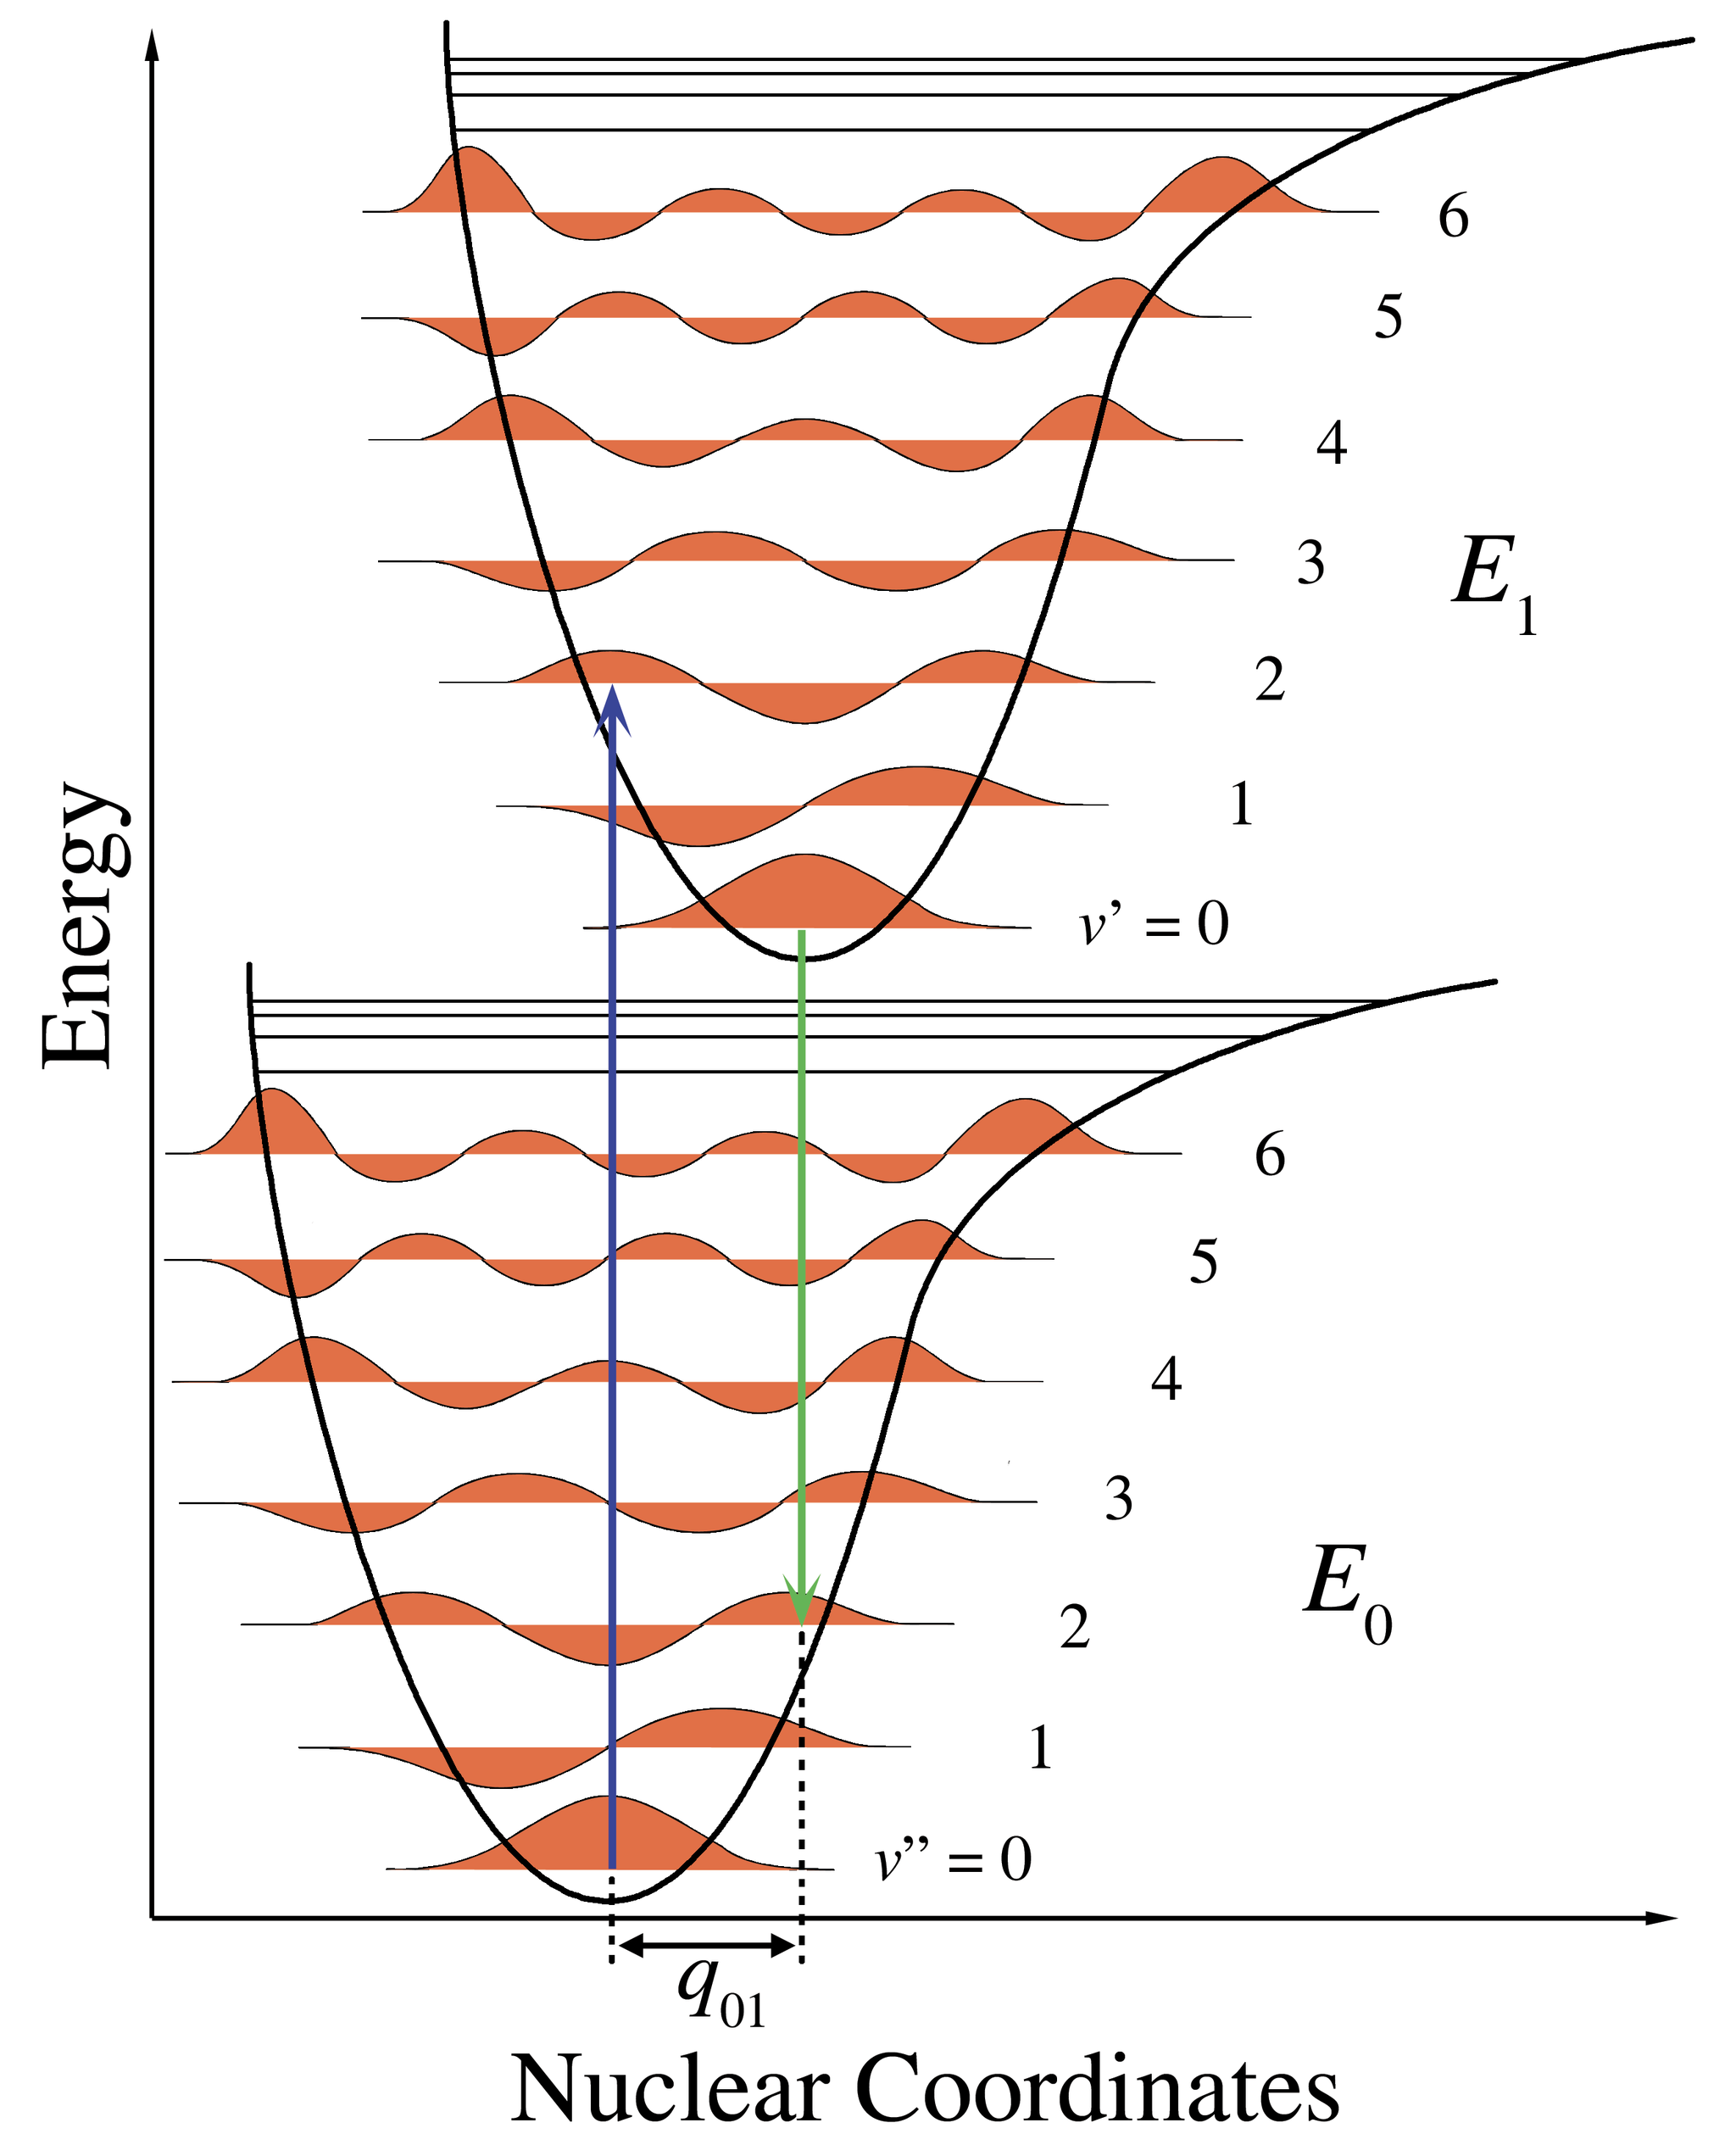
\includegraphics[width=0.6\linewidth]{images/FrankCondon} 

}

\caption{The vertical line of the absorption transition as the electron is promoted from the ground state to the excited state. The probability of the electron being excited into each vibrational level is given by the ‘overlap’ of the wave functions of ground and each excited state. Franck-Condon Diagram  (https://commons.wikimedia.org/wiki/File:Franck-Condon-diagram.png). From Wikimedia Commons, created by [Mark M. Somoza](http://www.gnu.org/licenses/fdl-1.3.html), CC-BY-SA-[3.0](https://creativecommons.org/licenses/by-sa/3.0/). Sept 14. }\label{fig:FrankCondon}
\end{figure}

The greater the overlap integral between the ground and excited state the higher the molar extinction coefficient and the more strongly coloured the molecule.

Understanding the variation of possible electronic transitions available when electronic levels are mixed with vibrational and rotational levels, as well as the molecular dynamics allowing multiple `non-minimised' structures explains the relative broadness of molecular electronic absorption and emission spectra.

\begin{figure}

{\centering 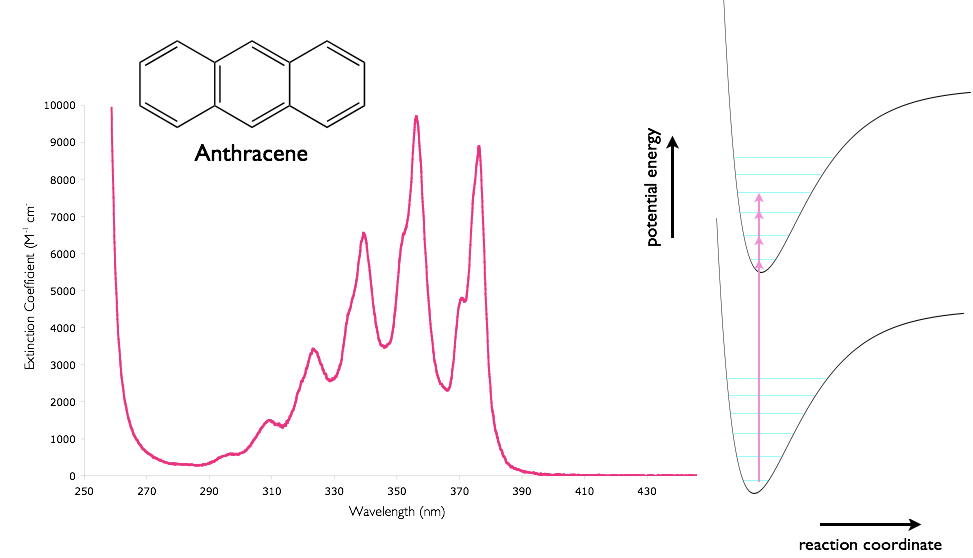
\includegraphics[width=0.9\linewidth]{images/Anthracene} 

}

\caption{The absorption spectra of anthracene in cyclohexane showing the vibrational fine structure, combined with a sketch of the potential energy wells of the ground and excited states. Regions with the highest molar extinction coefficient have the largest overlap integrals of the wavefunctions of the ground and excited states. }\label{fig:Anthracene}
\end{figure}

\hypertarget{sec:multiplicity}{%
\section{Multiplicity}\label{sec:multiplicity}}

If you recall Hunds' rule when filling atomic and molecular orbitals you will recall that the lowest energy state occurs when the spin of the electrons is aligned. Usually in an organic molecular orbital the HOMO is a fully occupied \(\pi\) set, or a fully occupied set of non bonding orbitals with all electrons paired.

It is common to refer to the electronic states in a molecule by their \emph{spin multiplicity}, given by \(2S+1\), where \(S\) is the sum of the electronic spins of the electrons in the orbital. For a species in which all of the electrons are paired \(S = 0\), and so \(2S+1 = 1\) and the state is referred to as a \emph{singlet}.

If two electrons are unpaired they will (in the lowest energy configuration) have parallel spins, the total spin \(S = 1\) and so the spin multiplicity, \(2S + 1 = 3\). This state is referred to as a \emph{triplet} state.

Species such as free radicals have one unpaired electron, consequently \(S = ½\), and \(2S + 1 = 2\), and the species is referred to as a \emph{doublet}.

Triplet states with the same electronic configuration (other than spin) have a lower energy than corresponding singlet states due to an effect called spin correlation. In triplet states the motion of the electrons in the orbitals are organised in such a way as to minimise the coulombic interactions between the charges, by minimising these coulombic interactions the energy of the system is also lowered.

Although formally flipping of electron spin is forbidden in photophysical and non photophysical processes it does occur. Processes that involve a change in electron spin are explained in later sections.

\hypertarget{sec:conjugationandenergygap}{%
\section{\texorpdfstring{Conjugation and the HOMO, LUMO energy gap, \(\Delta E\)}{Conjugation and the HOMO, LUMO energy gap, \textbackslash Delta E}}\label{sec:conjugationandenergygap}}

\begin{figure}

{\centering 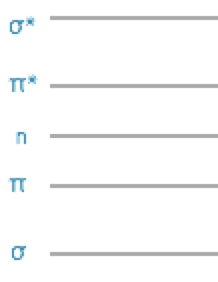
\includegraphics[width=0.2\linewidth]{images/nPiSigmaenergylevels} 

}

\caption{The relative energy arrangement of orbitals in a molecule, this simple sketch is usually good enough to gain an understanding of the system under investigation.}\label{fig:EnergyLevels}
\end{figure}

The greater the amount of conjugation in a molecule the smaller the energy gap between the HOMO \& LUMO and the longer the wavelength of photon absorbed.

This fits with the theory you learnt in your quantum mechanics lectures, where you can model the linear conjugated model quite accurately using the particle in a one dimensional box model.

\begin{longtable}[]{@{}
  >{\raggedright\arraybackslash}p{(\columnwidth - 6\tabcolsep) * \real{0.2500}}
  >{\raggedright\arraybackslash}p{(\columnwidth - 6\tabcolsep) * \real{0.2500}}
  >{\raggedright\arraybackslash}p{(\columnwidth - 6\tabcolsep) * \real{0.2500}}
  >{\raggedright\arraybackslash}p{(\columnwidth - 6\tabcolsep) * \real{0.2500}}@{}}
\caption{\label{tab:lambdaconj} The dependence of maximum absorption wavelength on the increasing length of conjugation is clearly shown by moving along the diene, triene, polyene series. Inclusion of a hetero atom with lone pairs introduces non-bonding, \(n\), electrons into the MO, and a second absorption band \(n \longrightarrow \pi^\ast\) introduced with a lower energy transition.}\tabularnewline
\toprule
\begin{minipage}[b]{\linewidth}\raggedright
\end{minipage} & \begin{minipage}[b]{\linewidth}\raggedright
\(\lambda\)\textsubscript{max} / nm \(\pi \longrightarrow \pi^\ast\)
\end{minipage} & \begin{minipage}[b]{\linewidth}\raggedright
\end{minipage} & \begin{minipage}[b]{\linewidth}\raggedright
\(\lambda\)\textsubscript{max} / nm \(n \longrightarrow \pi^\ast\) \(\pi \longrightarrow \pi^\ast\)
\end{minipage} \\
\midrule
\endfirsthead
\toprule
\begin{minipage}[b]{\linewidth}\raggedright
\end{minipage} & \begin{minipage}[b]{\linewidth}\raggedright
\(\lambda\)\textsubscript{max} / nm \(\pi \longrightarrow \pi^\ast\)
\end{minipage} & \begin{minipage}[b]{\linewidth}\raggedright
\end{minipage} & \begin{minipage}[b]{\linewidth}\raggedright
\(\lambda\)\textsubscript{max} / nm \(n \longrightarrow \pi^\ast\) \(\pi \longrightarrow \pi^\ast\)
\end{minipage} \\
\midrule
\endhead
& 217 & & 270 187 \\
& 227 & & \\
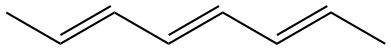
\includegraphics{images/octatrienestructure.png} & 263 & & 324 219 \\
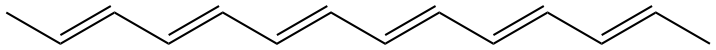
\includegraphics{images/longene.png} & 353 & & \\
\bottomrule
\end{longtable}

\hypertarget{sec:selectionrules}{%
\section{Selection rules for absorption \& emission processes}\label{sec:selectionrules}}

In molecular systems the most important selection rule is \(\Delta S = 0\), or there can be no change in the spin multiplicity during an absorption or emission processes, or there can be no `flipping' of electrons spin during a transition. In practice `coupling' due to interactions between the spin of the electron and the orbital mean that this selection rule is not rigidly followed.

In organic molecules containing only C, H, N \& O the direct absorption from S\textsubscript{0} to T\textsubscript{1} is so weak that it can't be seen in the absorption spectra. This `spin-orbit coupling' is more pronounced for heavier elements and molecules containing particularly heavy atoms, such as S, Cl or Br have more relaxed adherence to the \(\Delta S = 0\) selection rule.

The Laporte selection rule is more relevant when looking at inorganic transition metal complexes, or for atomic spectra which will not be considered in this work. The Laporte states that there must be a change in angular momentum quantum number, \(l\), upon absorption or emission in a cento symmetric system, or \(\Delta l = \pm 1\). So in a centro symmetric molecule, such as {[}Ti(H\textsubscript{2}O)\textsubscript{6}{]}\textsuperscript{3+}, figure \ref{fig:Tisplitting}, the allowed transitions would be transitions such as the following:

\begin{equation*}
1s \longrightarrow 2p \hspace{2cm}\textrm{or} \hspace{2cm} 1s \longrightarrow 3p
\end{equation*}

Whilst these transitions would be forbidden according to the Laporte rule:

\begin{equation*}
1s \longrightarrow 2s \hspace{2cm}\textrm{or} \hspace{2cm} 1s \longrightarrow 3d
\end{equation*}

Consequently the \(d-d\) transitions, such as the \(t_{2g} \longleftrightarrow e_g\) transition in octahedral complexes, which give most transition metal complexes are forbidden according to the Laporte rule.

\textbackslash begin\{figure\}

\{\centering 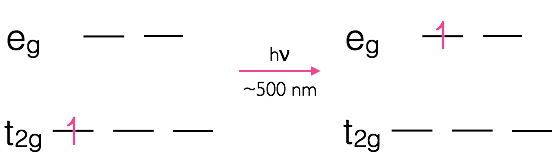
\includegraphics[width=0.6\linewidth]{images/Ti3splitting}

\}

\textbackslash caption\{The ligand field splitting of the 3d orbitals in a {[}Ti(H\(_2\)O)\(_6]\)\^{}\{3+\}\$ complex the solution is pale purple with a molar extinction coefficient, ε \textasciitilde{} 6.1 M\textsuperscript{−1} cm\(^{−}1\)\}\label{fig:Tisplitting}
\textbackslash end\{figure\}

If we compare the magnitude of of the molar extinction coefficient for a typical \(d-d\) absorption of a transition metal complex with that of a `spin allowed' `Laporte allowed' organic dye molecule we can see the effect of `non allowed' transitions. In table \ref{tab:extcoeff}, the organics, DNA \& the synthetic dye TOTO-1 both have extended conjugated molecular orbitals, and the transitions are from singlet to singlet, an allowed transition.

In these cases the Laporte rule does not apply as there is no centre of symmetry. The two examples of transition metal complexes {[}Cu(H\textsubscript{2}O)\textsubscript{6}{]}\textsuperscript{2+} \& {[}Ti(H\textsubscript{2}O)\textsubscript{6}{]}\textsuperscript{3+}, have significantly lower molar extinction coefficients.

Molar extinction coefficients, if you recall, were a representation of the orbital overlap between the HOMO \& LUMO, or a measure of how `allowed' the transition is. The transitions which are Laporte forbidden are at least two orders of magnitude less intense than the allowed transitions of the organic molecules.

Interestingly, permanganate which is relatively highly coloured when compared to other transition metal complexes cannot have colour due to \(d-d\) transitions as the +7 oxidation state of the manganese ion leaves no electrons in either the \(s\) or \(d\) orbitals. Instead the colour is due to a charge transfer transition, where upon absorption of a photon an electron is briefly transferred from one of the oxygen ligands to the manganese metal centre. Ligand to metal charge transfer complexes (and the associated metal to ligand charge transfer complexes), are not subject to selection rules and so are relatively intense.

\begin{longtable}[]{@{}lll@{}}
\caption{\label{tab:extcoeff} The molar extinction coefficients of a range of molecules, the magnitude is strongly dependent upon the adherence to selection rules, the two organic molecules, DNA bases \& TOTO-1 are both `spin allowed', permanganate is a LMCT which has no selection rules, whereas the final three molecules all fall foul of the Laporte selection rule which states \(\Delta l = \pm 1\). Since these transitions are `forbidden' the molar extinction coefficient is considerably lower than the allowed transitions.}\tabularnewline
\toprule
& \(\lambda\)\textsubscript{max} / nm & \(\varepsilon _{\lambda}\) / M\textsuperscript{-1} cm\textsuperscript{-1} \\
\midrule
\endfirsthead
\toprule
& \(\lambda\)\textsubscript{max} / nm & \(\varepsilon _{\lambda}\) / M\textsuperscript{-1} cm\textsuperscript{-1} \\
\midrule
\endhead
DNA (per base) & 260 & 6600 \\
TOTO-1 & 514 & 117000 \\
KMnO\textsubscript{4} & 520 & 1800 \\
CuSO\textsubscript{4} & 810 & 20 \\
{[}Ti(H\textsubscript{2}O)\textsubscript{6}{]}\textsuperscript{3+} & 500 & 6.1 \\
PrCl\textsubscript{3} & 445 & 0.07 \\
\bottomrule
\end{longtable}

The weak absorption carries on for the lanthanide complexes where \(f-f\) transitions are again forbidden by the Laporte selection rule. However, Ce\textsuperscript{3+} and Tb\textsuperscript{3+} have more intense electronic absorption bands which appear in the UV.

These are due to {[}Xe{]}4\(f\)\textsuperscript{n} to {[}Xe{]}4\(f\)\textsuperscript{n-1}5\(d\)\textsuperscript{1} transitions. Since the electron is moving from an \(f\) orbital to an \(d\) orbital it is not forbidden by the Laporte selection rule and so is considerably more intense than the forbidden \(f-f\) transitions. These transitions occur for these to ions due tooth stability provided by either an empty of half filled subshell.

\hypertarget{sec:structureonabs}{%
\section{Structure and Bonding Upon Absorption of a Photon}\label{sec:structureonabs}}

\begin{figure}

{\centering 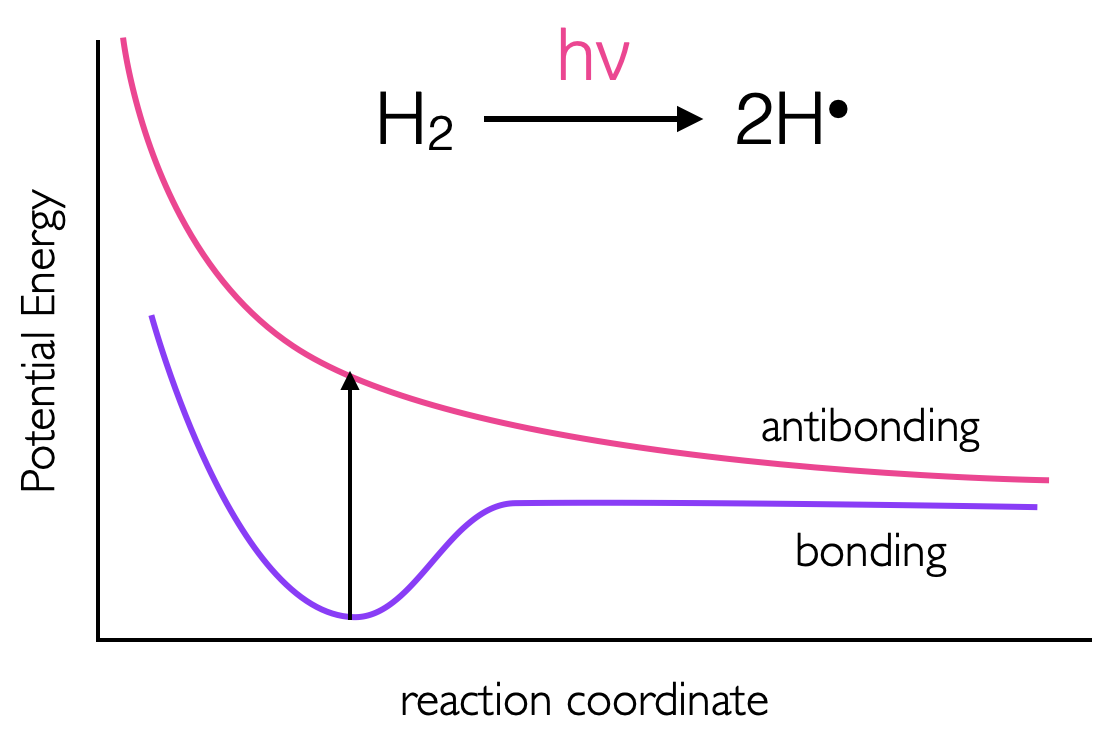
\includegraphics[width=0.6\linewidth]{images/Hbondingen} 

}

\caption{The energies of  bonding and anti bonding orbitals of molecular hydrogen, as an electron is prompted to the anti bonding σ* orbital the bond order is reduced to zero and the molecule ‘falls apart’..}\label{fig:Hbondingen}
\end{figure}

\begin{figure}

{\centering 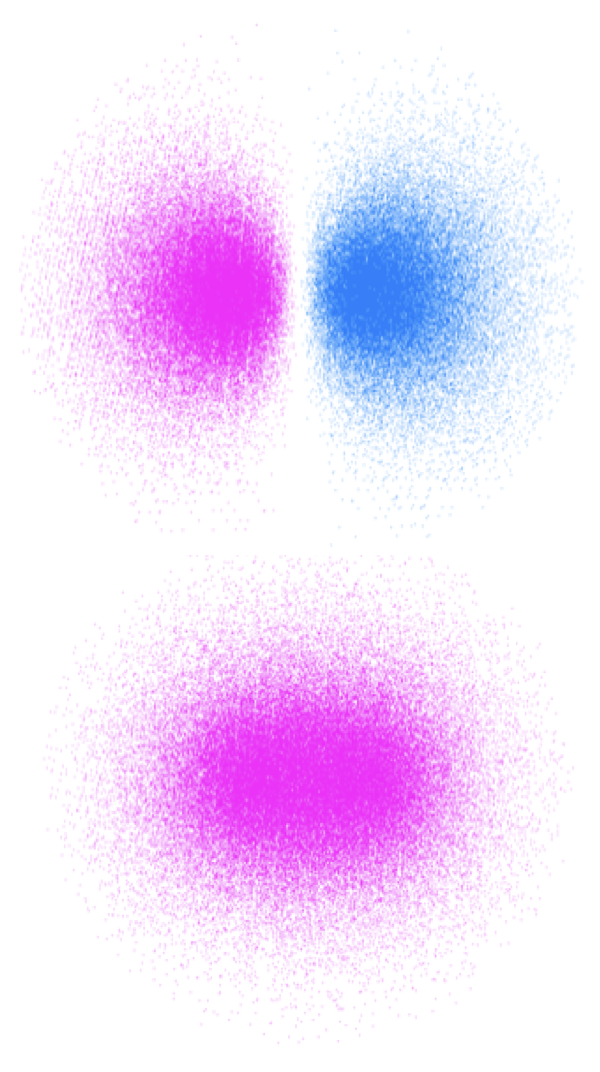
\includegraphics[width=0.3\linewidth]{images/Hbondingorb} 

}

\caption{The bonding and anti bonding orbitals of molecular hydrogen showing the node along the σ bond for the anti-bonding orbital.}\label{fig:Hbondingorb}
\end{figure}

Upon absorption of a photon, if an electron is promoted to an anti bonding orbital there is a reduction in the bond order. For a hydrogen molecule, with just two electrons, this leads to radical formation figures \ref{fig:Hbondingen} \& \ref{fig:Hbondingorb}.
It should be remembered that there is still an electron in the bonding orbital and the molecular orbital is now a blend of the HOMO and LUMO. The LUMO
For molecules with \(\pi\) electrons excitation of an electron to a \(\pi ^\ast\) orbital reduces the bond order to just 1, allowing for rotation around the previously restricted bond. If ethene is excited, the sp\textsuperscript{2} hybridised carbon, takes upon character of sp\textsuperscript{3} allowing rotation around the C-C bond, and changing the H-C-H bond angles. Rotation around a double bond is the basis of many photochemical reactions and is fundamental to vision where retinol, a long conjugated molecule undergoes a cis-trans isomerisation after excitation.

\hypertarget{sec:transdipole}{%
\section{The Transition Dipole Moment}\label{sec:transdipole}}

One thing which hasn't yet been considered is how light physically interacts with a molecule.

Classically it could be considered that the oscillating electric field of a wave could interact with a molecule if there was some resonance of the of the frequency of light and the frequency of oscillation of the electron in an orbital, it would seem obvious that an electron (carrying an electric charge) and an electromagnetic wave (with its oscillating electric field) should interact; and will interact given the correct wavelength. In simple terms the frequency of light and the energy gap for the transition were the same.

The classical model also explains why it is electrons which are excited (and not protons in the nucleus) because the considerably lighter electrons are more affected (and moved more) in the presence of the electric field.

This approach whilst covering the very basics of a transition does not particularly explain concepts such as the molar extinction coefficient, nor does it particularly consider concepts fundamental to quantum mechanics - such as quantisation of energy - an oscillating electric field is in no way quantised and there is no reason why excitation of the molecule should be quantised either.

However this idea of an oscillating dipole has some relation to quantum mechanics; because the shape of the molecular orbitals of the HOMO and LUMO are different and there will be a change in the electron distribution and hence a change in dipole of the molecule upon excitation. As such we can define a transition dipole moment for each chromophore - the more similar the ground and excited states the larger the transition dipole moment for the molecule.

A mathematical derivation of the transition dipole moment is beyond the scope of this work\footnote{see Principles of Photochemistry by Turro \emph{et al} if you wish to know more}, but it is worth discussing as transition dipoles are hugely important when it come to energy transfer in molecules (see Förster Resonance energy transfer, Section @ref(\{sec:forster\}).

If we consider light as a wave polarisation is well understood, however there is a quantum mechanical explanation for polarisation as well - in short we can use wave behaviour to consider polarisation and photon behaviour to explain quantisation - just to stick with concepts which should be familiar to us.

Light is only absorbed by a molecule if the polarisation of the light aligns with the transition dipole moment on the molecule. Figure \ref{fig:CS2} shows CS\textsubscript{2} a simple linear molecule - where the transition dipole moment runs along the long axis of the molecule.

\begin{figure}

{\centering 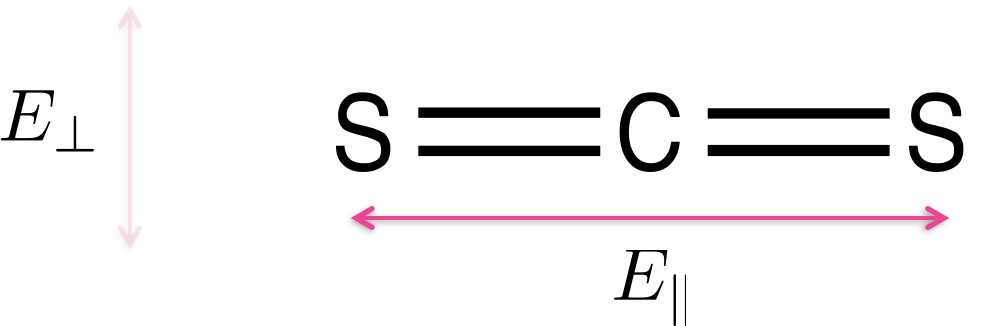
\includegraphics[width=0.6\linewidth]{images/CS2} 

}

\caption{Carbon disulfide (CS~2~) is a linear molecule -  due to the shape of the molecule there is a transition dipole which runs down the length of the long axis. Light aligned such that the electric field runs parallel with the long axis of the molecule E~||~ will be absorbed, light which in which the electric field runs perpendicular to the long axis of the molecule E~⊥~ will not be absorbed.}\label{fig:CS2}
\end{figure}

For more complicated molecules each of the transitions from the HOMO, HOMO-1 to the LUMO \emph{etc.} occur with different transition dipole moments across the chromophore, figure @ref\{fig:adenosine\}. Each transition is only excited when light is aligned with that transition; in most cases this isn't something we need to consider as most incident light we consider is isotropic, but alignment of transition dipoles (either between light and molecules - or between two different molecules) is an important consideration.

\begin{figure}

{\centering 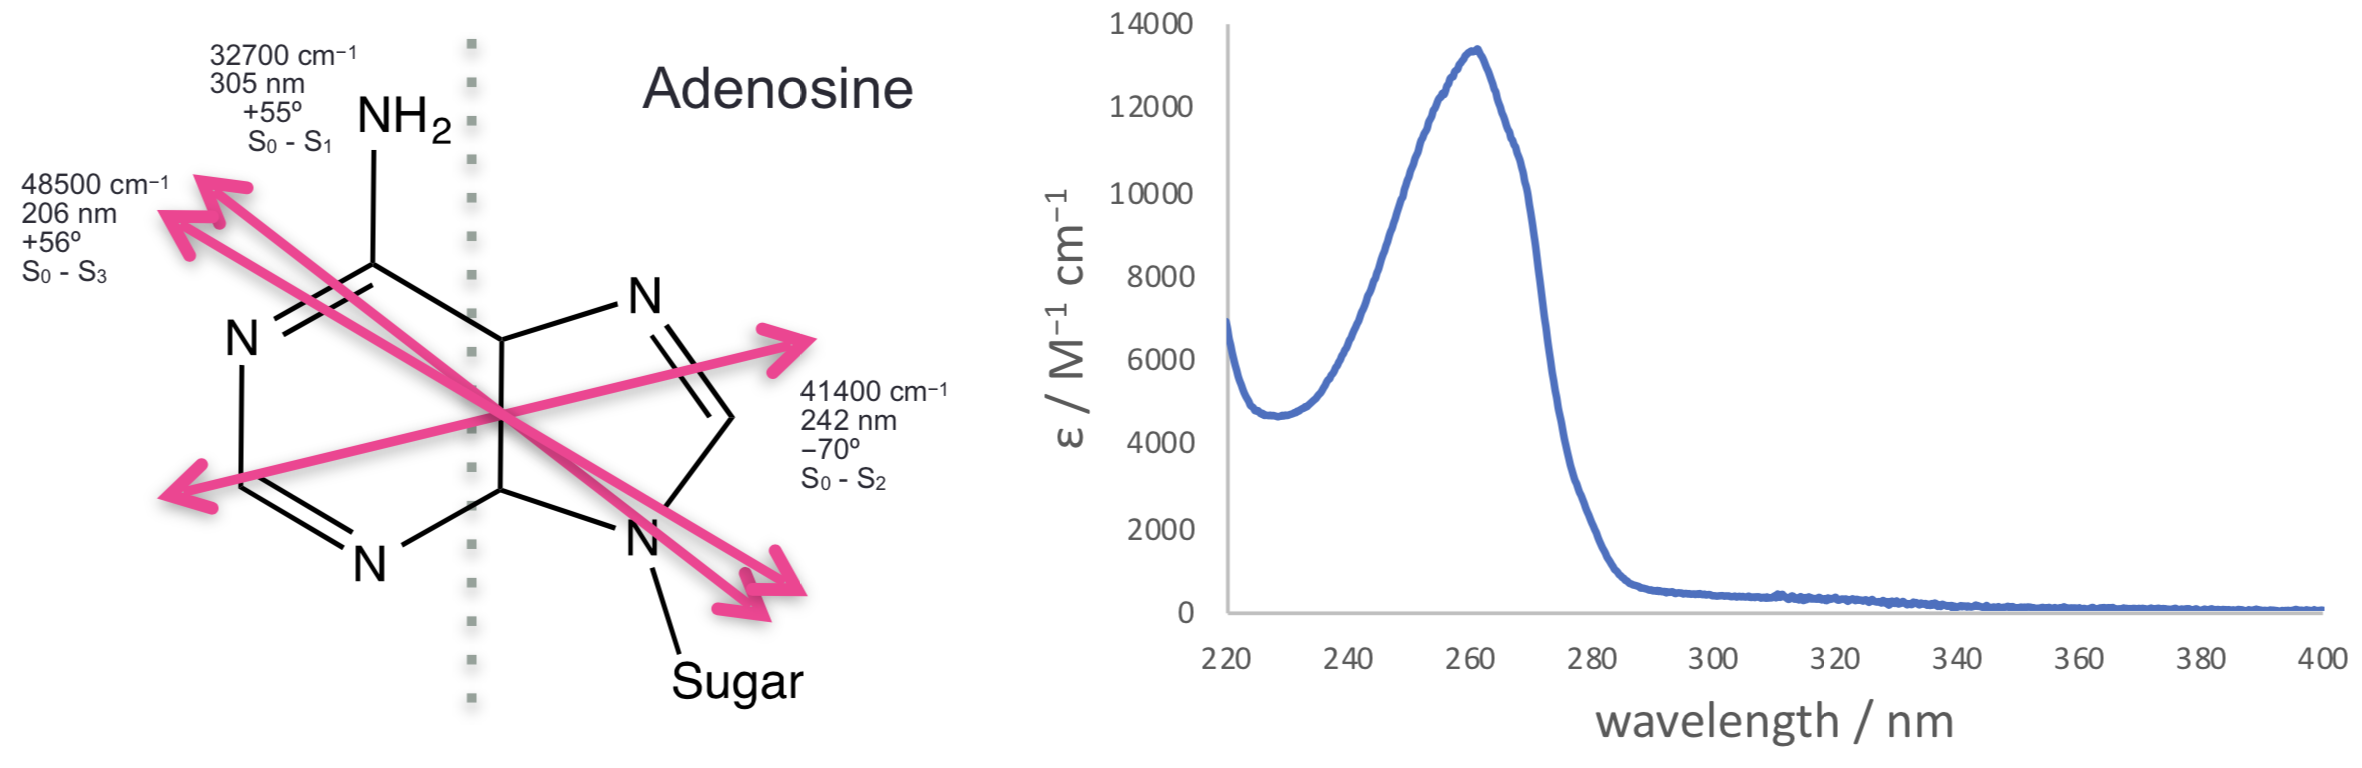
\includegraphics[width=1\linewidth]{images/adenosine} 

}

\caption{The three lowest energy transitions of adenosine each indicated with their transition dipole moment (all in the plane of the molecule, calculated values).These match with the observed spectrum with a weak transition around 310 nm, a much stronger transition around 260 nm and a third transition starting at the edge of the measured spectrum. [Spectrum [Adapted from OMLC]( https:// omlc.org/spectra/PhotochemCAD/html/033.html), 31st October 2018]}\label{fig:adenosine}
\end{figure}

As already discussed the transition dipole moment is derived from the difference in electron density of the ground and excited state. Figure \ref{fig:PhenRubpy3} shows the HOMO and LUMO of an organic chromophore, and a metal complex MLCT state.

\begin{figure}

{\centering 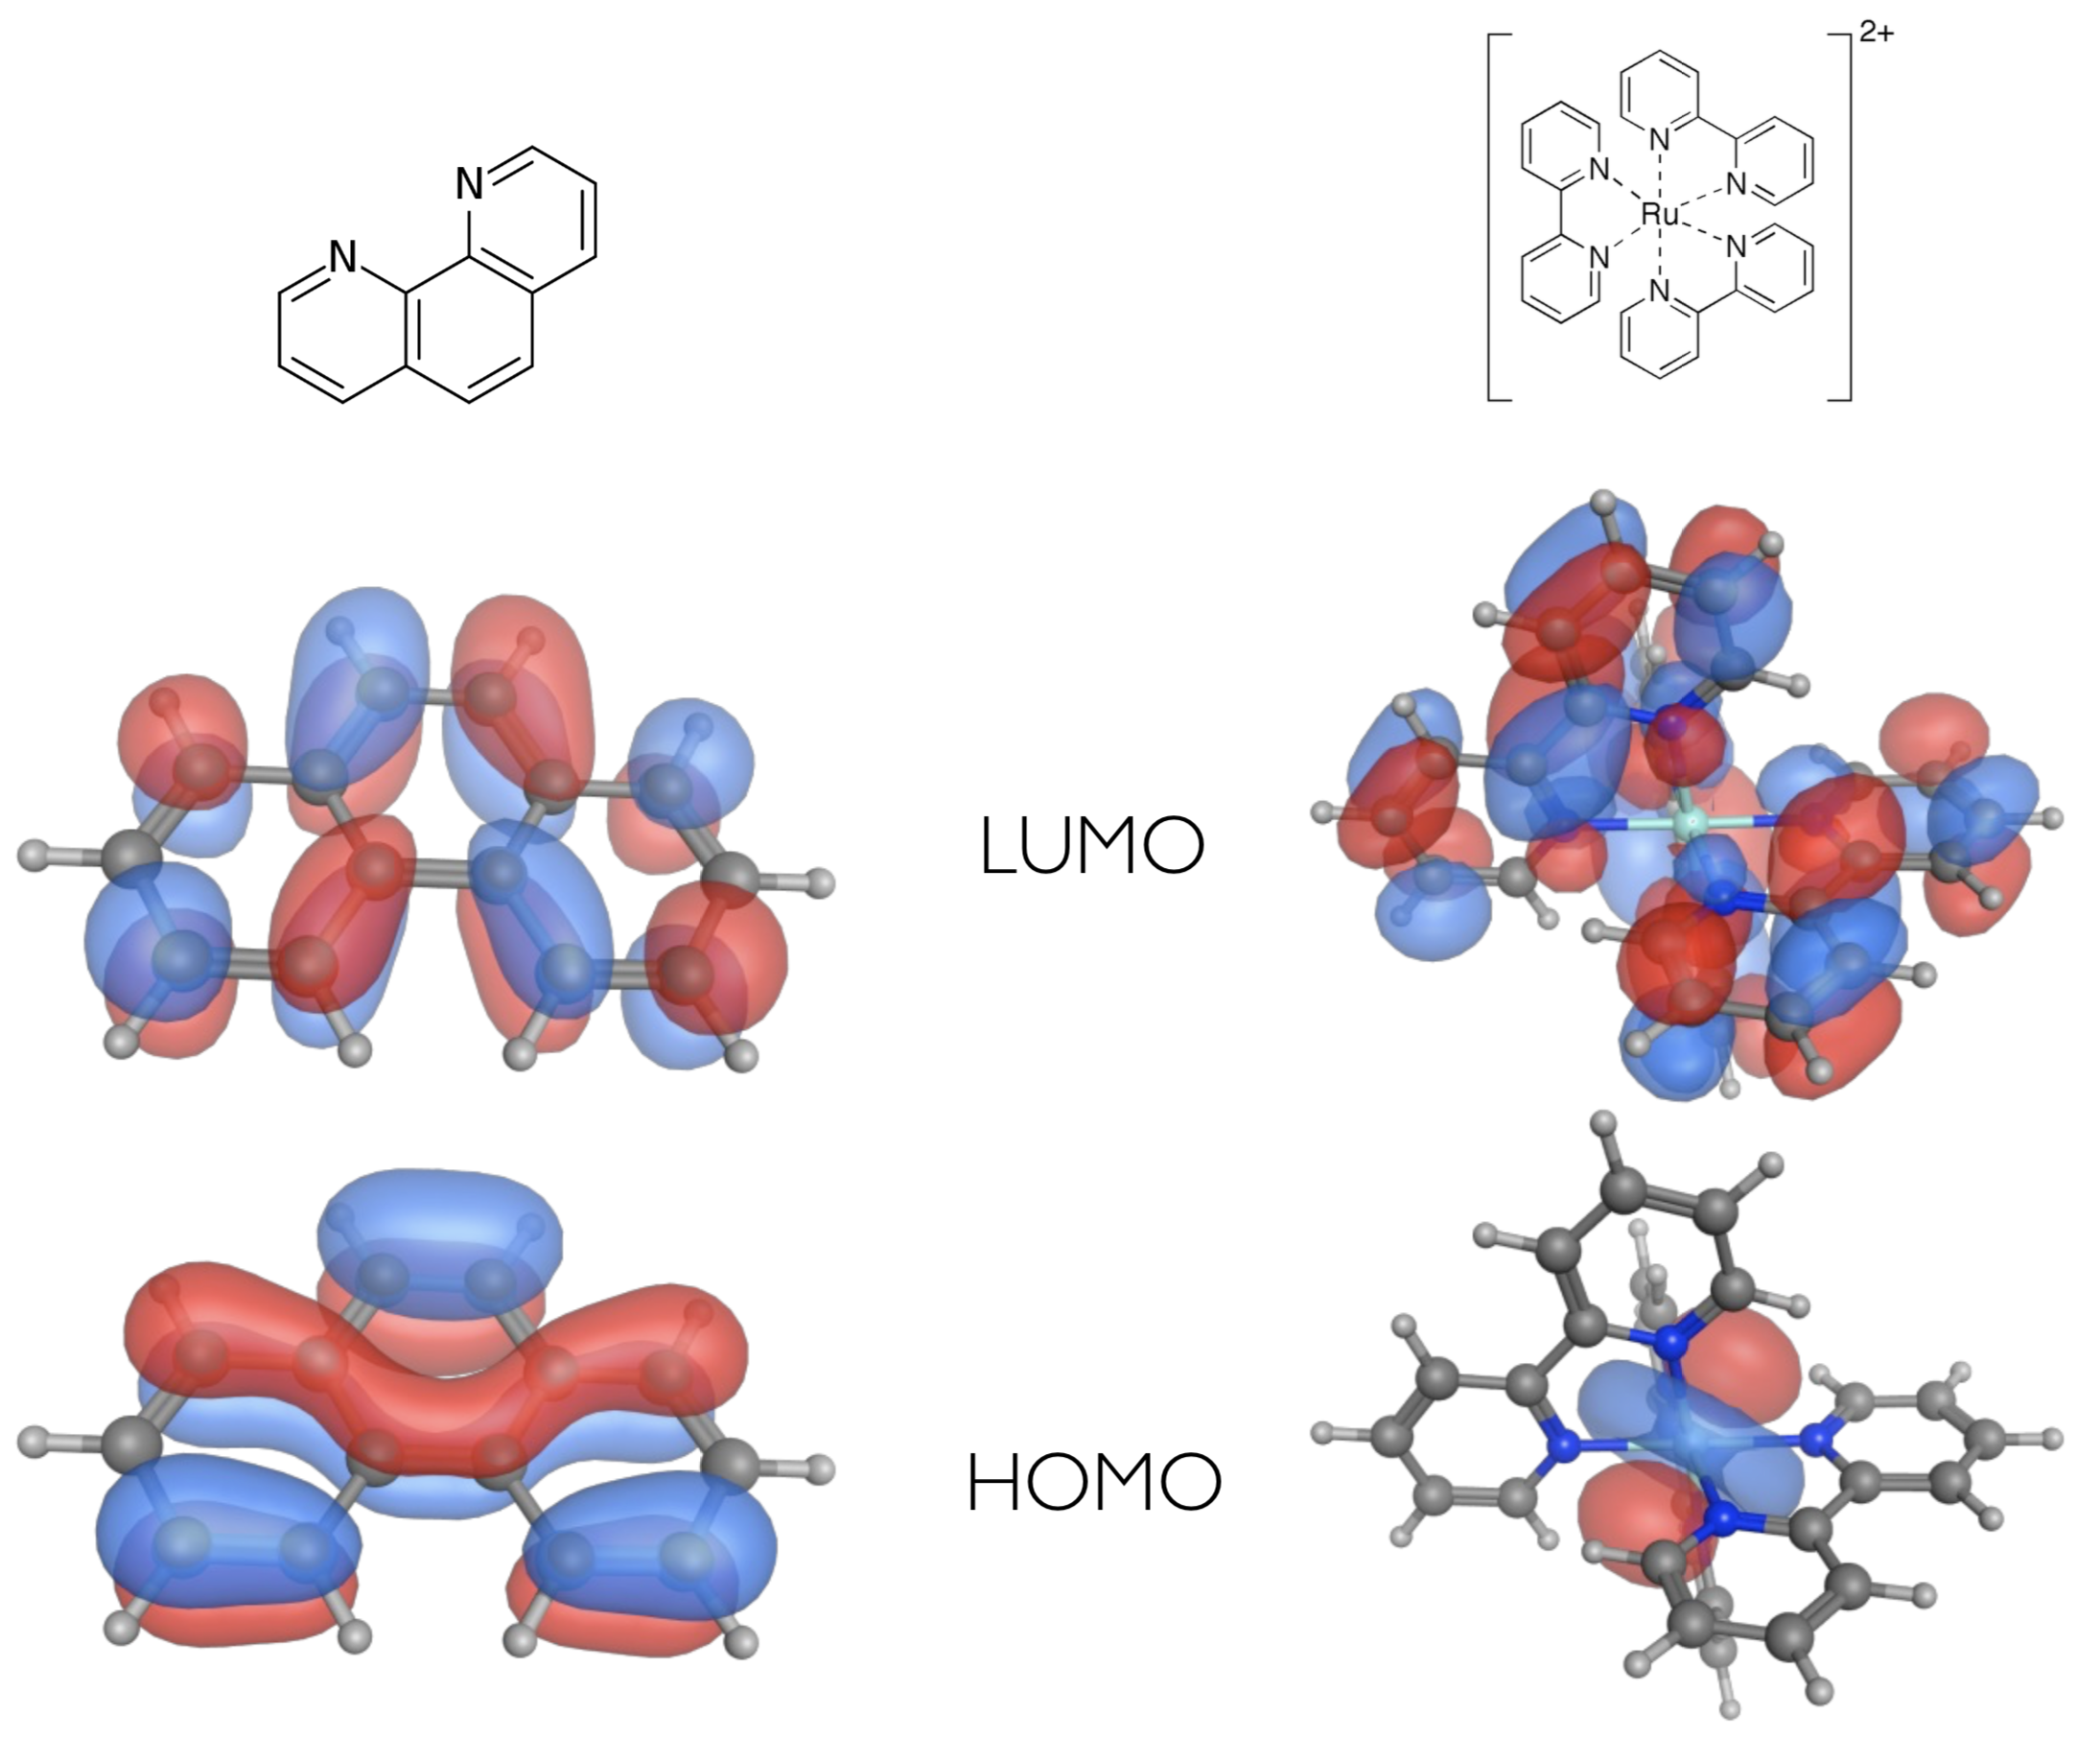
\includegraphics[width=1\linewidth]{images/PhenRubpy3} 

}

\caption{The calculated HOMO (bottom) and LUMO (top) of 1,10-phenanthroline (left) a model planar organic chromophore and [Ru (bpy)$_3$]$^{2+}$ (bpy - bipyridine) which has an MLCT state. For the ruthenium complex the HOMO is clearly centred on $4d_{z^2}$ orbital, whereas after absorption of a photon (and transfer of the electron) the electron density is then centred over the ligands in the LUMO.}\label{fig:PhenRubpy3}
\end{figure}

\hypertarget{factors-which-affect-the-absorption}{%
\section{Factors Which Affect the Absorption}\label{factors-which-affect-the-absorption}}

In the condensed phase the solvent is an important factor in determining the wavelength of maximum absorption, this effect, called solvatochromism, can be due to many properties of the solvent but is most likely due to solvent polarity. The LUMO energy level is unchanged in the different solvents, but the HOMO can either be more stabilised or less stabilised by the change in solvent (Figure \ref{fig:solvato}).

\begin{figure}

{\centering 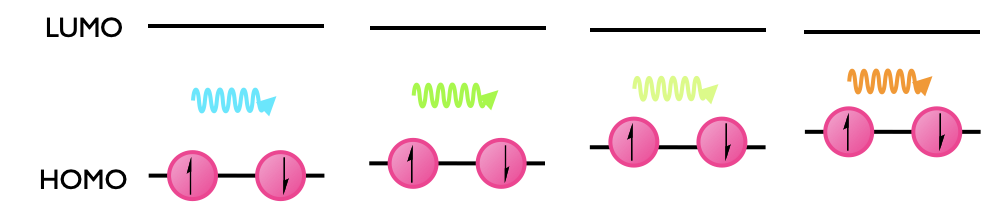
\includegraphics[width=1\linewidth]{images/Solvatochromism} 

}

\caption{The change in absorption wavelength as the HOMO is destabilised in a solvent series, here is worth noting that the colour observed and the wavelength of maximum absorption are not the same thing. As the HOMO is destabilised there is a red shift in the wavelength required to excite the electron.}\label{fig:solvato}
\end{figure}

This leads to a change in the HOMO LUMO energy gap and consequently a change in the wavelength of maximum absorption.

If the absorption maxima shifts to increasing wavelength (red shift, decreasing energy of transition) it is referred to as a bathochromic shift, whereas if the absorption maxima shifts to decreasing wavelength (blue shift, increasing energy of transition) it is referred to as a hypsochromic shift.

Another major factor that can affect the absorption of a sample are interactions between the chromophores. This is most commonly encountered with DNA, which shows a significantly higher absorption at high temperatures (Figure \ref{fig:DNAmelt}). This is because the bases of DNA `stack' to form the rungs of a ladder, this stacking has favourable \(\pi - \pi\) interactions which help to stabilise the macromolecule. As the DNA is heated the double helix begins to melt and the rigid ladder stack is broken. The favourable \(\pi - \pi\) interactions are lost and so the absorption increases. There is little or no change in the wavelength of the maximum absorbance in this process only an increase in the absorbance due to a higher value of molar extinction coefficient. This effect as the absorbance of DNA increases upon melting is called hyperchromicity, the converse, a decrease in absorption, is called hypochromicity.

\begin{figure}

{\centering 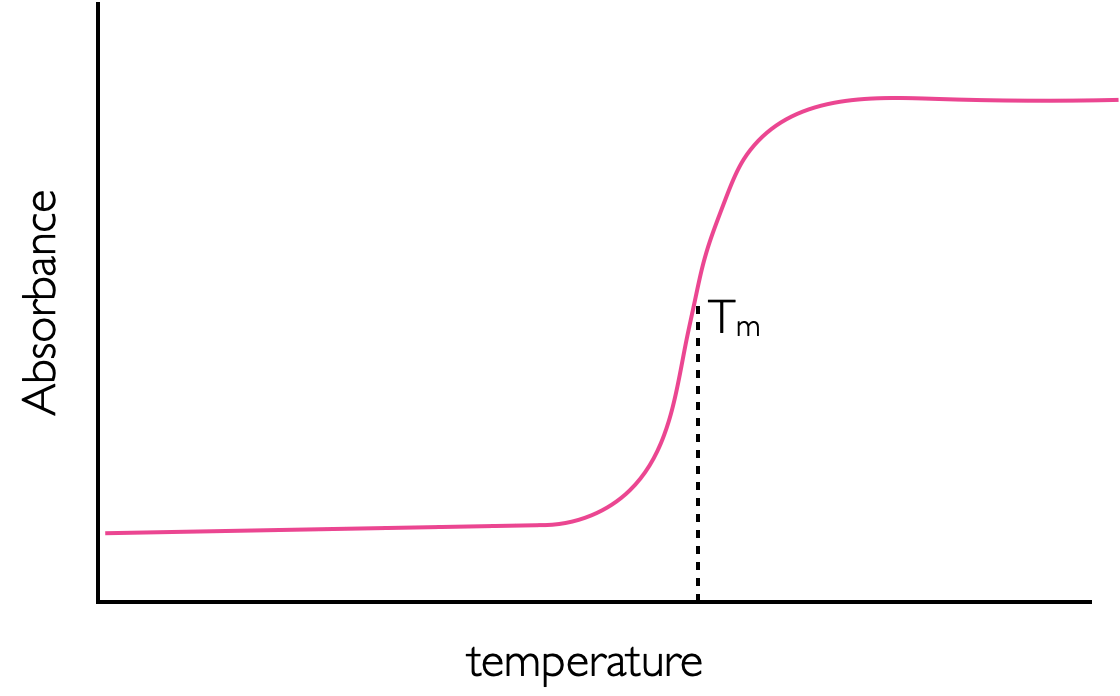
\includegraphics[width=0.6\linewidth]{images/DNAmelt} 

}

\caption{A sketch of the melting of DNA leading to a large increase in absorption. The melting temperature T~m~, is defined much as the end point of a titration curve is, as halfway between the two turning points. The increase in absorbance is due to the breaking of the π stack which exists in double stranded helical DNA.}\label{fig:DNAmelt}
\end{figure}

\hypertarget{sec:before1}{%
\section{Before Completing this Section}\label{sec:before1}}

To support the material in this section it is suggested you read chapter 2 of Wardle `Principles and Application of Photochemistry' and the section in Atkins' `Physical Chemistry' on Einstein coefficients. If you need a refresher of some MO theory it is recommended you look at the early chapters of Chemistry\textsuperscript{3}.

\hypertarget{sec:SSQabs}{%
\section{Self Assessment Exercises}\label{sec:SSQabs}}

\begin{enumerate}
\def\labelenumi{\arabic{enumi}.}
\tightlist
\item
  What would happen if an electron was excited from the HOMO to LUMO of ethane?
\item
  Why is the C-H bond angle 120º in the excited state of ethyne?
\item
  What would you expect to happen to the shape of ethene when and electron is excited from a \(\pi\) to \(\pi^\ast\) orbital?
\item
  Use the Beer-Lambert law to define the fraction of incident light that is absorbed by a solution of concentration c, in a cuvette of path length l.
\item
  Suggest why samples with absorptions greater than 1 tend not to be used by photochemists.
\item
  Use the Beer-Lambert law to calculate the fraction of incident monochromatic light absorbed by a 0.100 mM solutions of dye in a 1 cm cuvette, where the molar extinction coefficient of the dye is 3000 M\textsuperscript{−1} cm\textsuperscript{−1} (mol\textsuperscript{−1} dm\textsuperscript{3} cm\textsuperscript{−1}).
\item
  Sketch the linear combination of s-orbitals that give rise to the bonding and anti-bonding orbitals in molecular hydrogen.
\item
  How far can monochromatic 489 nm light travel through a 0.100 M solution of fluorescein with an extinction coefficient at 489 nm of 92000 M\textsuperscript{−1} cm\textsuperscript{−1} before 90 \% of it is absorbed?
\end{enumerate}

\hypertarget{sec:SSQabsans}{%
\section{Self Assessment Exercises brief answers}\label{sec:SSQabsans}}

\begin{enumerate}
\def\labelenumi{\arabic{enumi}.}
\item
  Ethane has no \(\pi\) electrons, so the HOMO is a \(\sigma\) bonding orbital and promotion of an electron would lead to an electron in an anti bonding \(\sigma^\ast\) orbital, and thus a bond order of 0, or the bond will break, forming a radical.
\item
  The carbon atoms in the linear ethyne molecule are of course sp hybridised. Excitation of an electron from a \(\pi\) orbital to a \(\pi^\ast\) orbital effectively changes the hybridisation so that it is more like sp\textsuperscript{2}. In consequence, the shape of the molecule changes from linear to bent.
\item
  Similarly a \(\pi\) to \(\pi^\ast\) excitation of ethene removes the C-C double bond character allowing rapid rotation of the hydrogen atoms. The carbon atoms appear in effect to be sp\textsuperscript{3} hybridised. In fact the up and down positions of the hydrogen can fluctuate so rapidly that the molecule still seems planar. In the case of ethane, excitation of the electrons in the orbitals leads to rupture of the bond, forming two CH\textsubscript{3} radicals.
\item
  \(\log_{10} \frac{I_{transmitted}}{I_{incident}} = - \varepsilon cl\) so that:
\end{enumerate}

\(\frac{I_{transmitted}}{I_{incident}} =10^{- \varepsilon cl }\)

\(I_{transmitted} = I_{incident} \times 10^{- \varepsilon cl }\)

\(I_{absorbed} = I_{incident} - I_{transmitted} = I_{incident} ( 1 - 10^{- \varepsilon cl })\)

fraction absorbed \(= \frac{I_{absorbed}}{I_{incident}} = 1 - 10^{- \varepsilon cl }\)

\begin{enumerate}
\def\labelenumi{\arabic{enumi}.}
\setcounter{enumi}{4}
\item
  Samples with an absorption of 1 have 90\% of the incident light absorbed, samples with an absorption of 2 have 99\% of incident light absorbed, leaving just 1\% of incident light reaching the detector. So it all comes down to the increasing error in measurement, because A is a calculated value based on the transmission a relatively weak incident light beam (because you don't want to degrade the sample), the error becomes massive when the absorption is still quite low. Even with modern instruments, which will record an absorption of 7 or 8, the noise becomes a huge issue. There are other issues with highly absorbing samples which lead to deviations from the Beer Lambert law, so samples should always be relatively dilute.
\item
  For the example, \(cl = 3000 \times 10^{-4} \times 1 = 0.3\), so that the fraction of incident light absorbed is
  \(1 - 10^{-0.3} = 0.5\), \emph{i.e.} about 50\% of the light is absorbed.
\item
  Two in phase combinations will lead to the formation of the bonding orbital, whereas two out of phase will lead to formation of the anti-bonding orbital, which has a node between the two nuclei.See figure \ref{fig:Hbondingorb}.
\item
  If 90\% of the incident light is being absorbed then 10\% of the light is transmitted\ldots{}
\end{enumerate}

\(\log \frac{I_0}{I}=\varepsilon cl\)

\(l=\frac{ \log \frac{I_0}{I}}{\varepsilon c}\)

\(l=\frac{\log \frac{100 \%}{10 \%}}{92000 \textrm{ M}^{−1} \textrm{ cm}^{−1} \times 0.100 \textrm{ M}}\)

\(l=\frac{1}{9200000 \textrm{ M}^{−1} \textrm{ m}^{−1} \times 0.100 \textrm{ M}}\)

\(l = 1.0 \textrm{ μm}\)

\hypertarget{ch:Em}{%
\chapter{Emission of Light}\label{ch:Em}}

\hypertarget{sec:EmLOs}{%
\subsection{Learning Objectives}\label{sec:EmLOs}}

At the end of this block you should be able to:

\begin{itemize}
\item
  Define singlet and triplet states in terms of molecular orbitals
\item
  Explain the mirror symmetry observed in absorption/fluorescence spectra.
\item
  Construct and explain the Jablonski diagram.
\item
  Define the rates of the processes in the Jablonski scheme and give typical values for the rate constants.
\item
  Define singlet and triplet lifetimes and describe how they are measured.
\item
  Analyse decay curves to obtain lifetimes of excited states.
\item
  Define and derive the quantum yield of fluorescence and phosphorescence.
\item
  Discuss the heavy atom effect.
\end{itemize}

Only the light absorbed by a molecule can produce photochemical change in a molecule. If a species absorbs radiation then one particle is excited for each quantum of radiation absorbed. This concept of light having to be absorbed before anything else can happen is an obvious one, but is an important concept in itself, it goes on to define the concept of quantum yield of a process, effectively the proportion of excited states which `decay' to any given pathway.

\hypertarget{sec:FluorPhos}{%
\section{Fluorescence \& Phosphorescence}\label{sec:FluorPhos}}

Just as there are `spin forbidden' and `spin allowed' processes for absorption, when the molecule is in an excited state there are a allowed and forbidden path ways of deactivation of the excited state.

If we look at a Jablonski diagram, figure 19, which you should already be familiar with, it shows the range of photophysical deactivation pathways of an excited state.

A Jablonski diagram (figure \ref{fig:Jablonski}) usually uses a short hand to refer to the excited states, where a ground state, if it is a singlet, is referred to as S\textsubscript{0}, and each subsequent excited state is referred to as S\textsubscript{1}, S\textsubscript{2} \emph{etc}.

\begin{figure}

{\centering 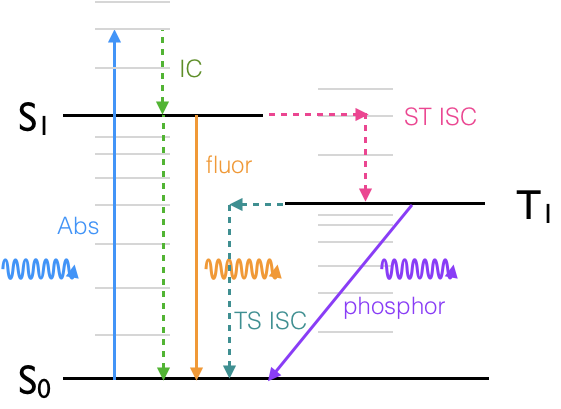
\includegraphics[width=0.7\linewidth]{images/Jablonski} 

}

\caption{Jablonski diagram showing: A, the absorption of a photon, and the photophysical deactivation pathways, IC, internal conversion, ISC, intersystem crossing, F, fluorescence \& P, phosphorescence.}\label{fig:Jablonski}
\end{figure}

Triplet states are referred to as T\textsubscript{1}, T\textsubscript{2}\ldots{} if the ground state is not a triplet then there is no state labelled T\textsubscript{0}. All excited states are referred to by integer vales of 1 or more.

\emph{A note on Jablonski diagrams: transitions which are either allowed or non-radiative and therefore not governed by selection rules appear as either horizontal or vertical transitions, forbidden transitions (such as phosphorescence) are indicated by transitions which occur at an angle. Radiative transitions (those that occur with either the absorption or emission of a photon) are shown as solid lines with the incident or excident photon shown as a wave like arrow. Non radiative transitions are shown as dashed (or alternatively wiggly) lines to clearly differentiate them from radiative transitions. Transitions with a change of spin are isoenergetic (shown as horizontal lines) before decaying via internal conversion (vertical lines). A Jablonski diagram is a sketch of the energy levels and should not include details of the potential wells of either the ground or excited state.}

The spin selection rule which applies for absorption transitions \(\Delta S = 0\), so formally emission transitions from the S\textsubscript{1} to S\textsubscript{0} are spin allowed, allowed emission transitions are referred to a fluorescence.

Emission transitions that involve a change in spin of the electron, such as from T\textsubscript{1} to S\textsubscript{0}, are spin forbidden, and referred to as phosphorescence. The excited state can also decay via non-radiative transitions and other routes.

Table \ref{tab:phototrans} the deactivation pathways from excited states:

\begin{longtable}[]{@{}
  >{\raggedright\arraybackslash}p{(\columnwidth - 4\tabcolsep) * \real{0.4286}}
  >{\raggedright\arraybackslash}p{(\columnwidth - 4\tabcolsep) * \real{0.2857}}
  >{\raggedright\arraybackslash}p{(\columnwidth - 4\tabcolsep) * \real{0.2857}}@{}}
\caption{\label{tab:phototrans} The excitation and decay pathways in molecules.}\tabularnewline
\toprule
\endhead
\emph{`Allowed transitions'} & & \\
Singlet-singlet absorption Singlet-singlet emission & fluorescence & \(S_0 + h \nu \longrightarrow S_1\) \(S_1 \longrightarrow S_0 + h \nu '\) \\
\emph{`Forbidden transitions'} & & \\
Singlet-triplet absorption Triplet-singlet emission & fluorescence & \(S_0 + h \nu \longrightarrow T_1\) \(T_1 \longrightarrow S_0 + h \nu ''\) \\
\emph{`Other transitions'} & & \\
Internal conversion & (vibrational relaxation) (vibrational relaxation) & \(S_1 \longrightarrow S_0 + heat\) \(S_1 \longrightarrow T_1 + heat\) \(T_1 \longrightarrow S_0 + heat\) \\
\emph{Other pathways} & & \\
Quenching of excited state Chemistry from excited state & & \(S_1 + Q \longrightarrow S_0 + Q +heat\) \(S_1 + Q \longrightarrow S_0 + Q^\ast +heat\) \(T_1 + Q \longrightarrow S_0 + Q +heat\) \(T_1 + Q \longrightarrow S_0 + Q^\ast +heat\) \(S_1 \longrightarrow\) new/changed molecule \\
\bottomrule
\end{longtable}

The spin selection rule has important consequences on the lifetime of singlet and triplet states. The spin allowed process of fluorescence usually has a short lifetime (less than 10 ns), whereas the spin forbidden process of phosphorescence has a significantly longer lifetime, which can be as long as several seconds.

Vibrational relaxation occurs in the ps timescale, consequently the excited state decays vibrationally to the S\textsubscript{1}, v' = 0 state and emission essentially always occurs from the ground vibrational electronically excited state. This is an important concept in photophysics and is called Kasha's rule.

\hypertarget{sec:Kasha}{%
\subsection{Kasha's Rule}\label{sec:Kasha}}

\emph{An excited state always emits from the lowest energy level of that spin multiplicity state.}

The Frank-Condon principle applies equally to emission processes and the excited state will decay to a number of available vibrationally excited states of the ground electronic state. After relaxation to the \(v’ = 0\) level emission occurs to each of the available vibrational states of the ground state. The relative intensity of each band depends upon the coupling or overlap integral between the ground and excited states, as shown in figure \ref{fig:anthracenekasha}.

\begin{figure}

{\centering 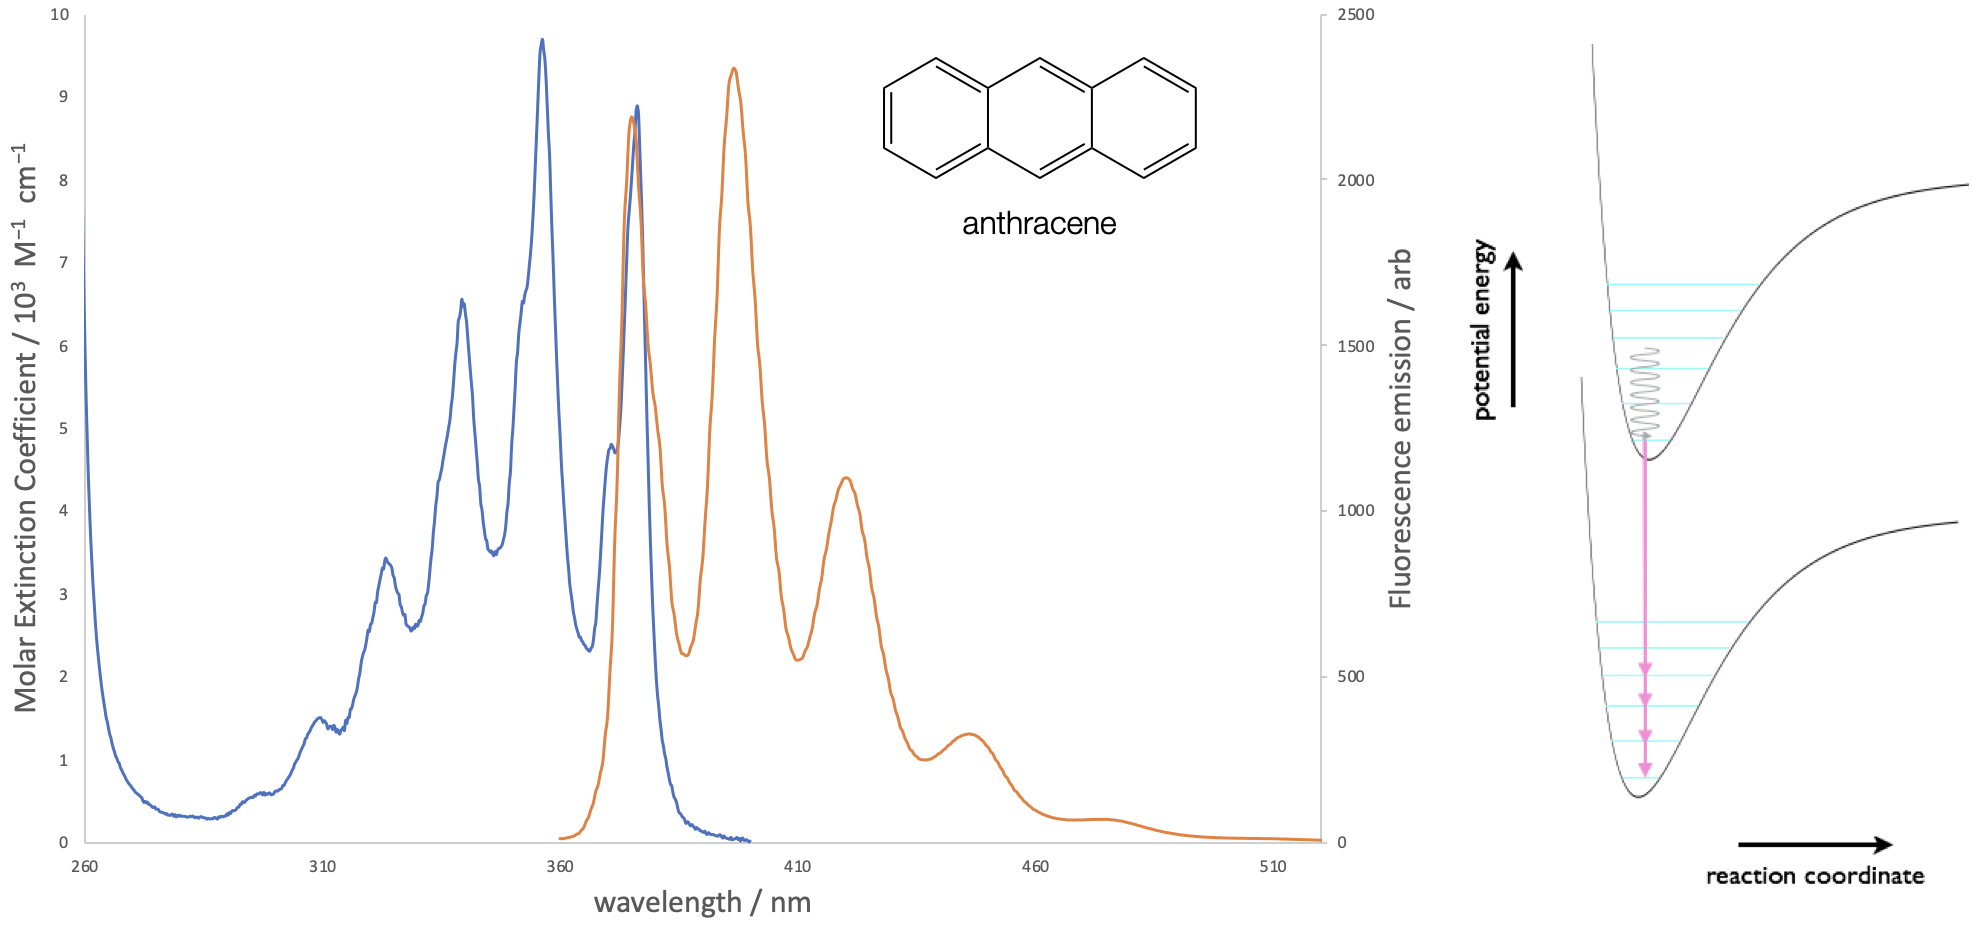
\includegraphics[width=0.7\linewidth]{images/anthracenekasha} 

}

\caption{The absorption and emission spectra of anthracene in ethanol solution. Both the absorption and emission spectra show vibrational fine structure, due to transitions to discrete vibrational energy levels in the excited and ground states respectively.}\label{fig:anthracenekasha}
\end{figure}

\hypertarget{sec:stoke}{%
\section{Stoke's shift}\label{sec:stoke}}

The Franck-Condon factors in absorption and emission is clearly evident by the symmetry shown in the emission of most organic chromophores. The Stoke's shift, the difference between the \(v=0\) to \(v’=0\) absorption peak and the \(v’=0\) to \(v=0\) emission peak, can simply be explained by the offset of the ground and excited state potential wells (figure \ref{fig:stokesspectrum}). Absorption happens from the centre of the \(v=0\) ground state and emission from the centre of the \(v’=0\) excited state, however this does not explain why the two curves are offset from one another.

\begin{figure}

{\centering 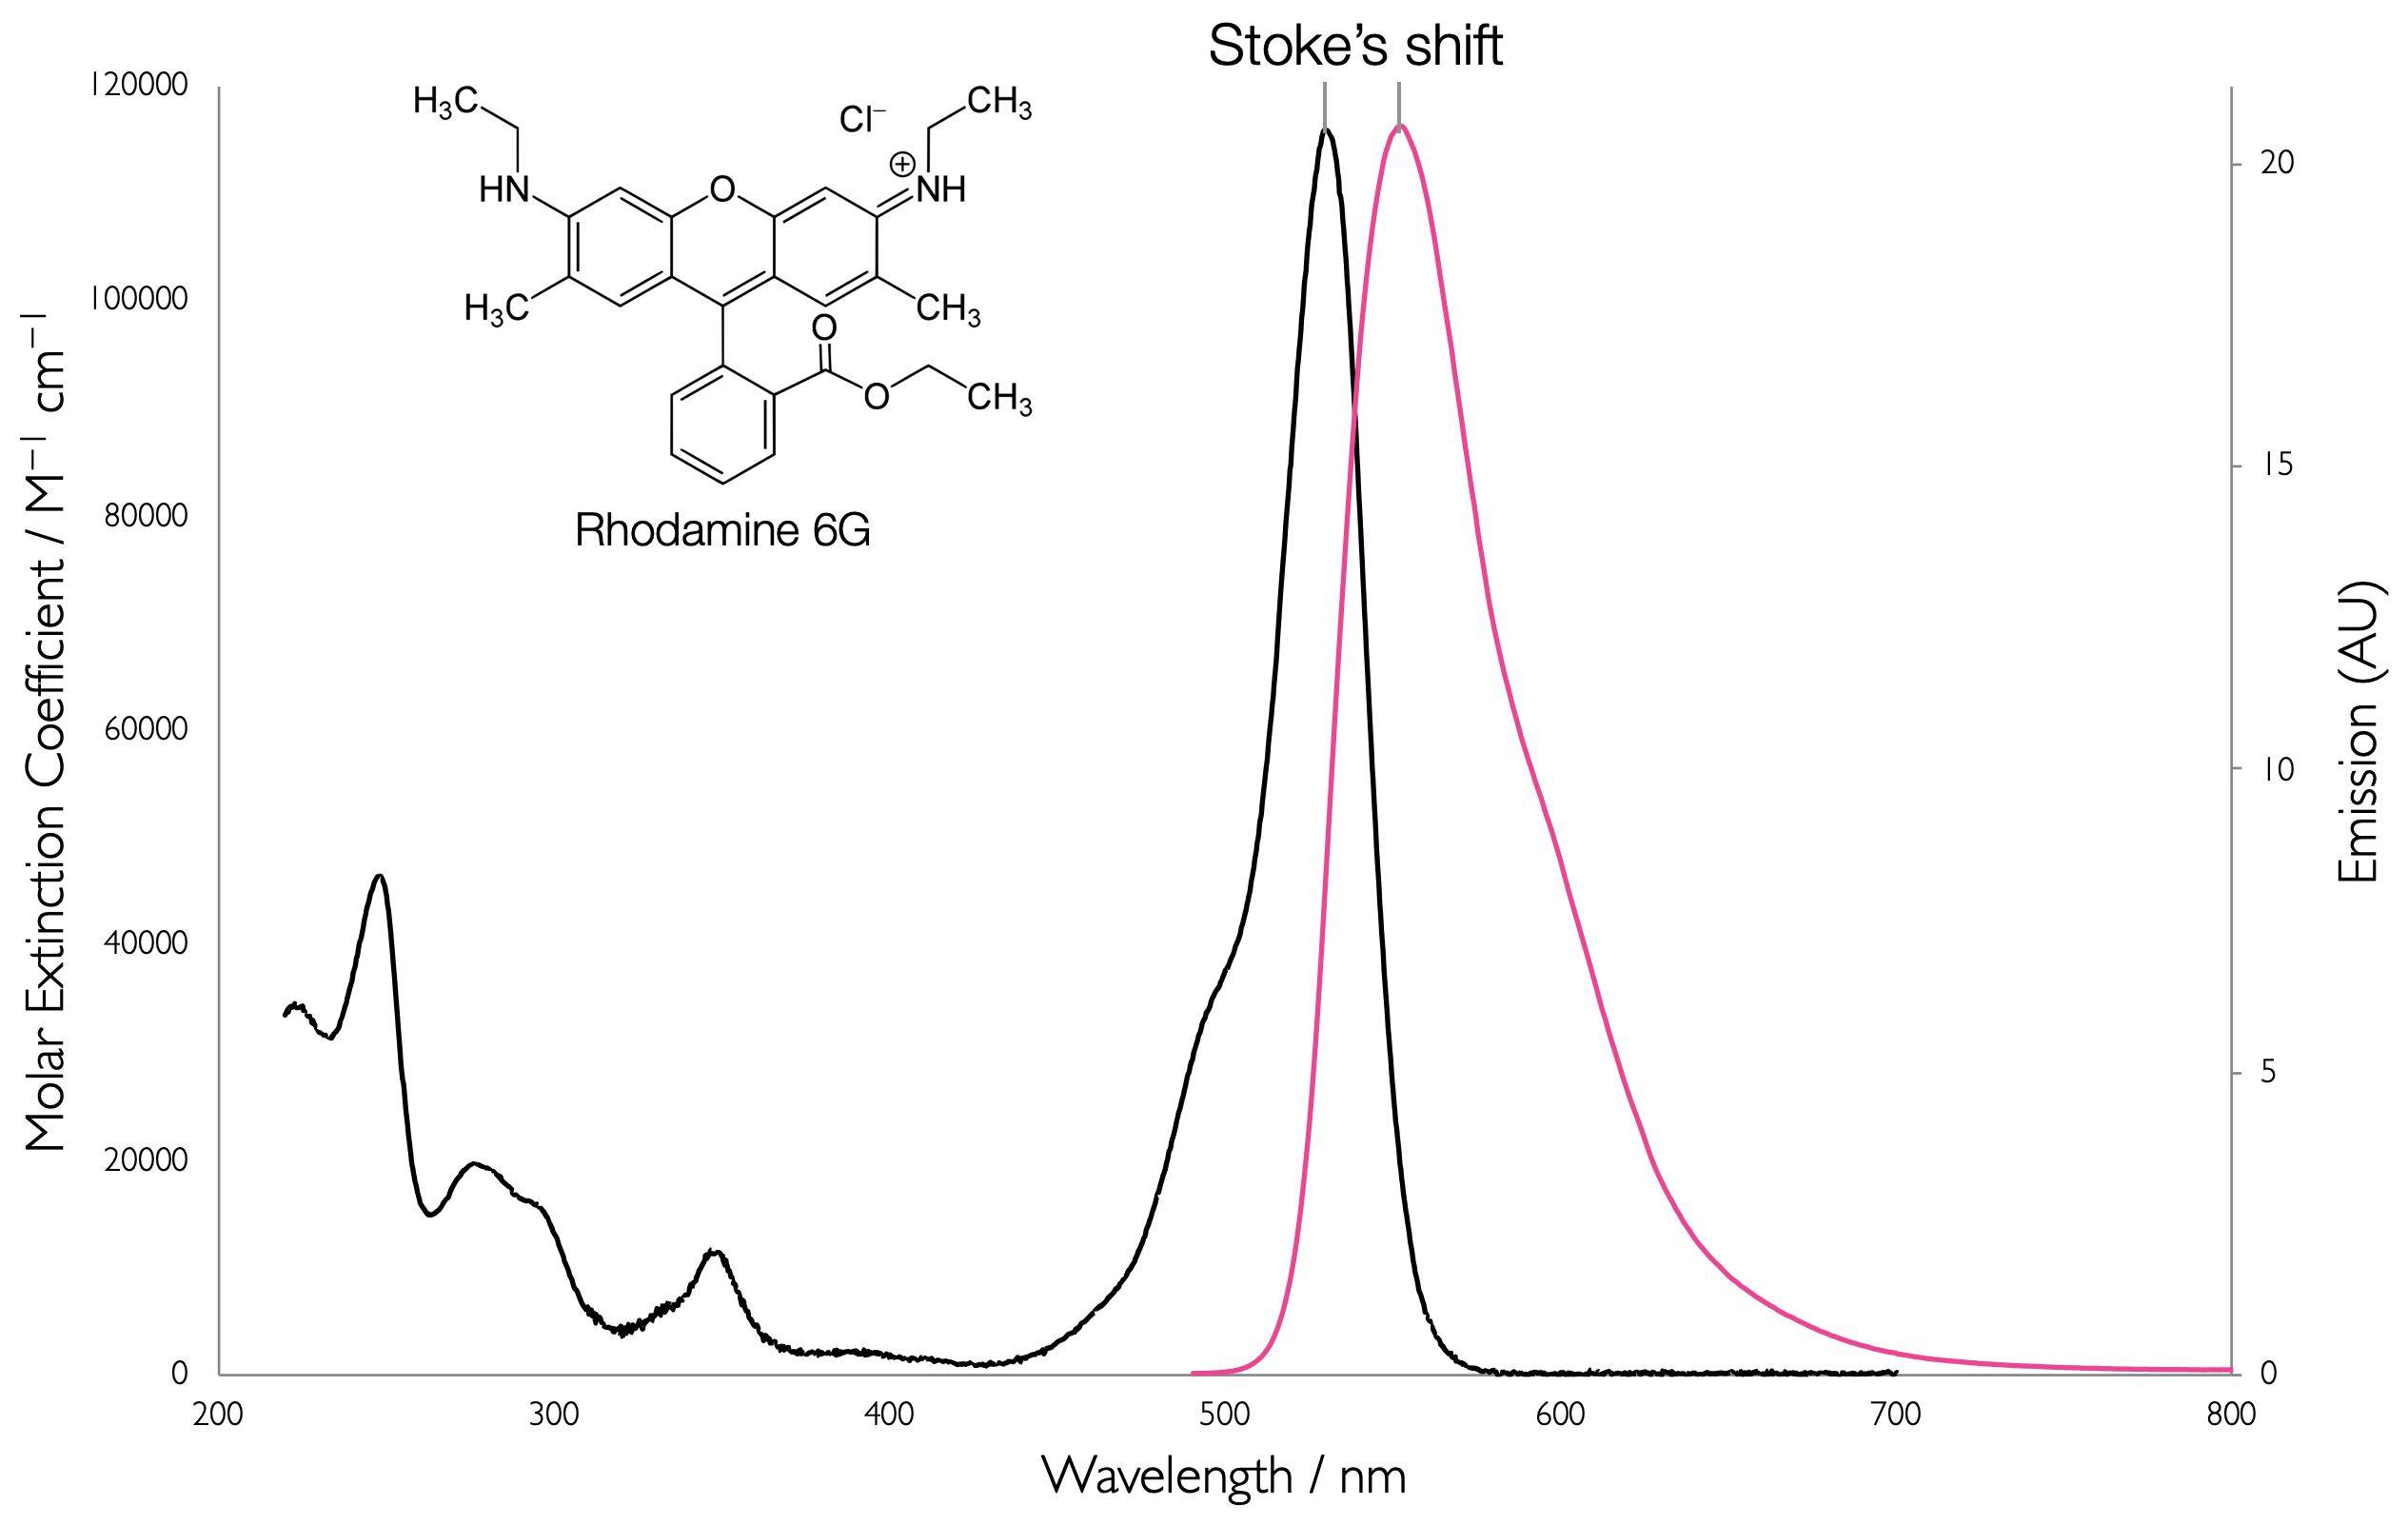
\includegraphics[width=0.7\linewidth]{images/stokesspectrum} 

}

\caption{The absorption and emission spectra of rhodamine 6G showing the Stokes shift of the two spectra.[Data from [OMLC](https://omlc.org/spectra/PhotochemCAD/html/083.html), accessed July 2020]}\label{fig:stokesspectrum}
\end{figure}

The axis title of 'reaction coordinate' is used ubiquitously, but is poorly understood. The simple idea that a bond becomes longer (as would be the case for a diatomic molecule) does not apply as we are considering the whole molecule.

The Stokes shift can be far more easily accounted for if we consider what is going on in the molecule. Initially the molecule exists in a state optimised for for that state, the shape and structure of the dye molecule and the arrangement of solvent around it are all minimised to give the lowest energy configuration. We shall consider the most simple case of the transitions between the ground vibrational states of the HOMO \& LUMO.

Absorption of a photon is a very fast process, in the order of femtoseconds, and is significantly faster than molecular vibrations or structural reorganisation. Consequently the molecule becomes excited into a state which has exactly the same structural configuration and salvation shell as the ground state, however this is now no longer the most optimal state, figure \ref{fig:stokesenergy}.

\begin{figure}

{\centering \includegraphics[width=0.8\linewidth]{images/stokesenergy} 

}

\caption{Sketch of the photophysical processes involved in the Stokes shift of emission. The ground state structure of the dye and solvent sphere (lower left) is maintained upon almost instantaneous absorption of a photon, however this then relaxes to an optimised configuration of dye and solvent for the excited state (top right), however this destabilises the ground state.}\label{fig:stokesenergy}
\end{figure}

Since the excited state is relatively stable (ns) when compared with the time taken for vibrations and molecular restructuring (ps) the excited state dye molecule and the solvent will reorganise to minimise the energy of the excited state, however in doing so this destabilises the ground state of the molecule. The actual process of emission is again very fast (ps) and so there is no opportunity for the structure of the chromophore or solvation sphere to reorganise. Upon deactivation this state, optimised for the excited state reorganises, lowering the energy of the ground state and destabilising the excited state.

As a consequence of this stabilising action of the ground and excited states the energy gap of absorption is larger than the energy gap of emission, or the emission of a photon is redshifted from the absorption. This explains the origin of Stokes shift, and explains the offset the Morse curves of the ground and excited states which have previously been used to explain the origin of the Stokes shift.

\hypertarget{sec:azuleneS2}{%
\section{\texorpdfstring{Emission from S\textsubscript{2}}{Emission from S2}}\label{sec:azuleneS2}}

Kasha's rule is almost always true, but there are known exceptions to this rule, one of these examples is azulene. Azulene has a broad absorption band between 500-600 nm, however emission from this molecule occurs at below 400 nm. If we look at figure \ref{fig:azulene} which shows the absorption and emission spectra of azulene it can be seen that the emission spectra is a mirror image of S\textsubscript{0}-S\textsubscript{2} (excitation into the second excited electronic state) absorption band, indicating the emission is also from the S\textsubscript{2} to S\textsubscript{0} states.

\begin{figure}

{\centering 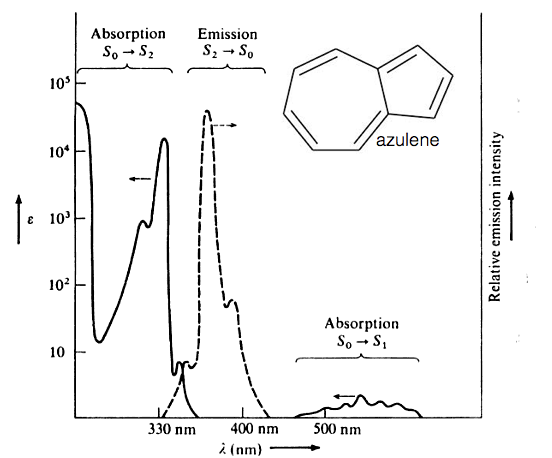
\includegraphics[width=0.6\linewidth]{images/azulene} 

}

\caption{The absorption (solid line) and emission (dashed line) spectrum of azulene in ethanol. Note the emission appears in the near UV part of the spectrum. }\label{fig:azulene}
\end{figure}

The molar extinction coefficient is also significantly higher for this S\textsubscript{0}-S\textsubscript{2} absorption indicating a much greater overlap integral of these two states.

What causes the unusual photophysical example? In short there is a very large energy gap between the S\textsubscript{2} and S\textsubscript{1} excited states this has the effect of greatly reducing the rate of internal conversion. There is a very weak emission from the S\textsubscript{1} to S\textsubscript{0}, in this case the energy gap is relatively small and there is an efficient deactivation of the excited state by internal conversion.

\hypertarget{sec:ratesphoto}{%
\section{Rates of Photophysical Processes \& Quantum Yield}\label{sec:ratesphoto}}

Fluorescence (and phosphorescence) are first order processes, just like radioactive decay. The probability of a molecule decaying from an excited state depends only the concentration of that excited state, \([A^\ast]\).

Rate of decay of \([A^\ast]\):

\begin{equation}
\frac{\textrm{d}[A^\ast]}{\textrm{d}t}=-k_f [A^\ast]
\label{eq:fluordecay}
\end{equation}

It is usual to refer to the `lifetime' of photophysical processes, and it is a term already used at the start of this chapter, the lifetime of a process, usually given the symbol τ, is the reciprocal of the rate constant for that process, so τ\textsubscript{f} = 1/k\textsubscript{f}. Often the natural lifetime of a dye is used, this assumes that there are no other deactivation pathways from the excited state and all of the energy is lost as fluorescence (or the fluorescence quantum yield is 1). The natural lifetime of fluorescence is given the symbol τ\textsubscript{f}\textsuperscript{0}, it is the maximum a lifetime can be and is solvent dependent.

If there is more than one possible deactivation pathway from the excited state is is often useful to be able to quantify these values. The quantum yield of a process describes the efficiency of each process, when a molecule absorbs a photon of light it generates an excited state; there are a number of different ways the molecule can decay from this excited state (see section \ref{sec:FluorPhos}, figure \ref{fig:Jablonski}). The quantum yield for each process is essentially the ratio of reactions proceeding down each pathway and the number of photons absorbed, quantum yield has no units.

\begin{equation}
\phi = \frac{\textrm{number of reactions proceeding down a given pathway}}{\textrm{number of photons absorbed}}
\label{eq:QYdef}
\end{equation}

\begin{longtable}[]{@{}
  >{\raggedright\arraybackslash}p{(\columnwidth - 6\tabcolsep) * \real{0.3778}}
  >{\raggedright\arraybackslash}p{(\columnwidth - 6\tabcolsep) * \real{0.2667}}
  >{\raggedright\arraybackslash}p{(\columnwidth - 6\tabcolsep) * \real{0.1778}}
  >{\raggedright\arraybackslash}p{(\columnwidth - 6\tabcolsep) * \real{0.1778}}@{}}
\caption{\label{tab:QYtab} The deactivation pathways of an excited state, with the associated rate constants and quantum yields.}\tabularnewline
\toprule
\begin{minipage}[b]{\linewidth}\raggedright
\end{minipage} & \begin{minipage}[b]{\linewidth}\raggedright
\end{minipage} & \begin{minipage}[b]{\linewidth}\raggedright
Rate of Process
\end{minipage} & \begin{minipage}[b]{\linewidth}\raggedright
Quantum Yield
\end{minipage} \\
\midrule
\endfirsthead
\toprule
\begin{minipage}[b]{\linewidth}\raggedright
\end{minipage} & \begin{minipage}[b]{\linewidth}\raggedright
\end{minipage} & \begin{minipage}[b]{\linewidth}\raggedright
Rate of Process
\end{minipage} & \begin{minipage}[b]{\linewidth}\raggedright
Quantum Yield
\end{minipage} \\
\midrule
\endhead
Absorption & \(S_0 + h \nu \longrightarrow S_1\) & \(I\) & \\
Fluorescence & \(S_1 \longrightarrow S_0 + h \nu'\) & \(k_f[S_1]\) & \(\phi _f\) \\
Internal conversion & \(S_1 \longrightarrow S_0 + \textrm{heat}\) & \(k_{ic}[S_1]\) & \(\phi _{ic}\) \\
Intersystem crossing \emph{singlet to triplet} & \(S_1 \longrightarrow T_1 + \textrm{heat}\) & \(k_{ST}[S_1]\) & \(\phi _{ST}\) \\
Phosphorescence & \(T_1 \longrightarrow S_0 + h \nu''\) & \(k_p[T_1]\) & \(\phi _p\) \\
Intersystem crossing \emph{internal conversion triplet to singlet} & \(T_1 \longrightarrow S_0 + \textrm{heat}\) & \(k_{TS}[T_1]\) & \(\phi _{TS}\) \\
\bottomrule
\end{longtable}

According to the Stark-Einstein law the total quantum yield of all processes is unity (one), however if secondary reactions occur (such as radical propagation) it may be more than 1. The quantum yield and rate of a process are intrinsically linked. It should be implicit that the faster the rate of a process (the bigger the rate constant) the bigger the quantum yield of that process; in fact the quantum yield of a process, such as fluorescence, is the rate of fluorescence divided by the sum of the rates of all of the deactivation processes (equation \eqref{eq:QYfluor}).

\begin{equation}
\phi_f = \frac{k_f^0}{k_f^0+k_{ic}+ k_{ST}+k_{\textrm{other}}}
\label{eq:QYfluor}
\end{equation}

(Examples of expressions for other processes may be found in Section \ref{sec:SSQemissionans} equations \eqref{eq:QYIC}, \eqref{eq:QYST} \& \eqref{eq:QYTS}.)

When there are more processes occurring then the singlet lifetime (sometimes called the fluorescence lifetime) will be smaller than the natural fluorescence lifetime, because now the denominator term is bigger (equation \eqref{eq:lifetimefluor}).

\begin{equation}
\tau_S = \frac{1}{k_f^0+k_{ic}+ k_{ST}+k_{\textrm{other}}}
\label{eq:lifetimefluor}
\end{equation}

If we assume that there is no quenching of the system (this is discussed later) and no chemistry the only decay pathways from the excited state are emission (fluorescence), internal conversion and intersystem crossing to the triplet state, and so consequently only these terms would appear in the equation for the quantum yield. Processes that occur from the triplet state are independent, and therefore none of these terms occur in quantum yield or lifetime equations from the singlet, fluorescent state.

For processes that occur from the triplet state, then obviously, the quantum yield will depend upon the total number of triplet states produced, which is given by the quantum yield of intersystem crossing. So the quantum yield of phosphorescence is given by:

\begin{equation}
\phi_p = \frac{k_p^0}{k_p^0+k_{TS}+k_{\textrm{other}}}
\label{eq:QYphos}
\end{equation}

Quantum yields of photophysical processes can be difficult to measure, in part because it is difficult to easily quantify the number of photons going into a sample, and because emission occurs at all angles from the sample. A technique called `actinometry' is usually used where the emission from an unknown sample is compared with that of a well characterised sample.

A good actinometer should have a good overlap in both the absorption and emission spectra, a high molar absorption coefficient, it should be photochemically stable and have a high emission quantum yield, a selection of well characterised actinometers are included in figure \ref{tab:actinometer}. Measurements on the absorption at the excitation wavelength, and the full emission spectra are required for both the unknown and the actinometer, as well as details on the reactive index of the solvents used. For best results a monochromatic light source should be used (a laser) and the same excitation wavelength must be used for both samples; the absorbance of the solutions should also be low (\textless0.1).

Usually emission spectra are measured as intensity against wavelength, but when `integrating' the emission of the unknown and actinometer it is important that they are integrated over a linear space (energy or frequency) which can make calculations more difficult (but perfectly doable in something like Excel). Equation \eqref{eq:actinometry} shows the relationship between the fluorescence quantum yield of an unknown, Φ, with that of a reference actinometer, Φ\textsubscript{R}. A is the absorbance at the excitation wavelength, and n the refractive index of the solvent. Here, because all terms appear as ratios there is no need to worry about units with anything.

\begin{equation}
\phi=\phi_R \frac{\int{I}\textrm{d}\bar \nu}{\int{I_R}\textrm{d}\bar \nu}\frac{A_R}{A}\frac{n^2}{n^2_R}
\label{eq:actinometry}
\end{equation}

The integrated emission intensity, \(\int{I}\textrm{d}\bar \nu\), of the unknown and reference is here shown as being integrated over wavenumber, but so long as it is integrated over linear space\footnote{The term linear space implies the steps are the same size, energy is the more fundamental unit, since wavelength is a reciprical function of energy wavelength space is non linear.} it does not matter if frequency or energy is used instead as any units from the terms cancel.

\begin{longtable}[]{@{}lllll@{}}
\caption{\label{tab:actinometer} The photophysical details of well characterised actinometers.}\tabularnewline
\toprule
Reference & Solvent & λ\textsubscript{ex}/nm & Φ\textsubscript{em} & λ\textsubscript{em,max} / nm \\
\midrule
\endfirsthead
\toprule
Reference & Solvent & λ\textsubscript{ex}/nm & Φ\textsubscript{em} & λ\textsubscript{em,max} / nm \\
\midrule
\endhead
quinine sulfate & 0.1 M H\textsubscript{2}SO\textsubscript{4} & 350 & 0.577 & 444 \\
fluorescein & 0.1 M H\textsubscript{2}SO\textsubscript{4} & 496 & 0.95 & 521 \\
rhodamine 6G & ethanol & 488 & 0.94 & 530 \\
cresyl violet & methanol & 540 & 0.54 & 622 \\
\bottomrule
\end{longtable}

\hypertarget{fluorescence-lifetime}{%
\section{Fluorescence lifetime}\label{fluorescence-lifetime}}

Spontaneous emission (either fluorescence or phosphorescence) from an excited state is a first order process, and so shows similar kinetics to that which you have already studied, figure \ref{fig:fluorlifetime} \& equation \eqref{eq:fluorlifetime}.

\begin{figure}

{\centering 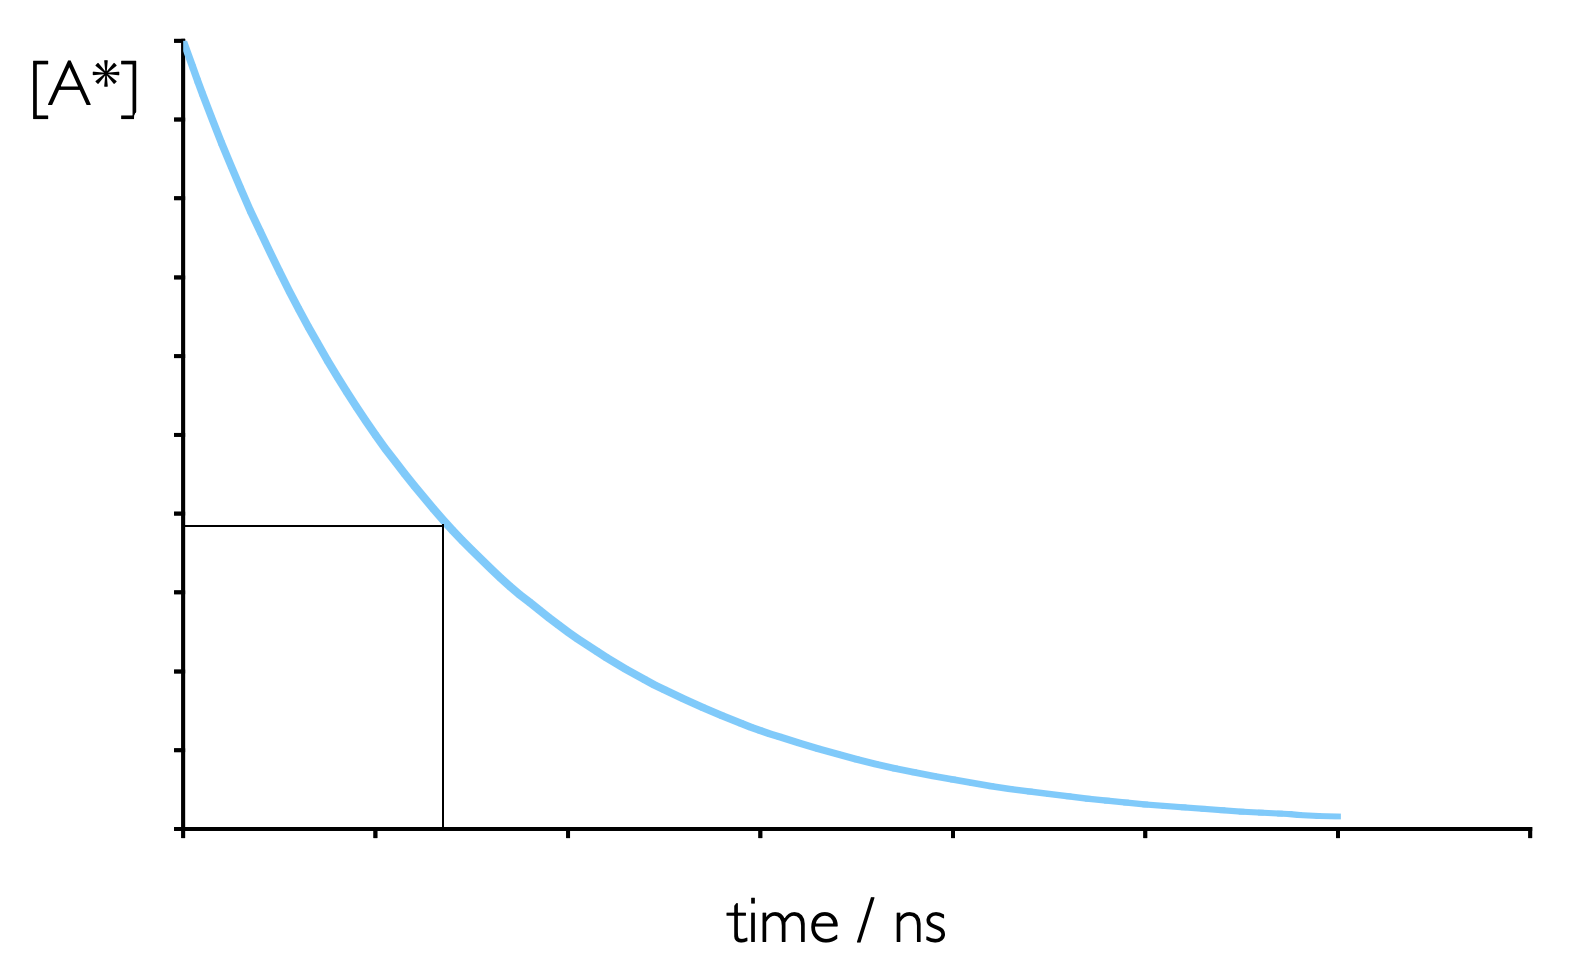
\includegraphics[width=0.5\linewidth]{images/fluorlifetime} 

}

\caption{Emission from an excited state is a first order process, whereby an excited state decays spontaneously. The emission lifetime is the time required for the concentratio of an excited state to fall to 1/e of its initial value.}\label{fig:fluorlifetime}
\end{figure}

However, instead of using rate constants when talking about this decay (as seen in Section \ref{sec:ratesphoto} photochemists tend to talk about emission lifetimes, \(\tau\).

The fluorescence lifetime is defined as the time required for the concentration of excited state to fall to 1/e (\textasciitilde0.3679) of the initial concentration.

So for an excited singlet state the fluorescence lifetime is related to the concentrations as follows:

\begin{equation}
[S_1]_t=[S_1]_0e^-{\frac{t}{\tau}}
\label{eq:fluorlifetime}
\end{equation}

where \(\tau\) is the value given in equation \eqref{eq:lifetimefluor}.

\hypertarget{sec:energygap}{%
\section{The Energy Gap Law}\label{sec:energygap}}

The natural lifetime of fluorescence assumes that there is no other available pathway for deactivation of the excited state. However, the effects of internal conversion and intersystem crossing have already been seen by the presence of rate constants for internal conversion (IC) and intersystem crossing (ST) in the equations for quantum yield of fluorescence. The rate of non-radiative decay is given by the energy gap law (a formalised equation is not given here) which depends upon a number of factors but principally the energy gaps (ΔE) between electronic levels.

Non radiative decay become increasingly unfavourable as the energy gaps become bigger, and the rate of non-radiative decay decreases exponentially with increasing energy gaps. The energy gaps between higher electronic states (S\textsubscript{2}, S\textsubscript{3}, S\textsubscript{4} \emph{etc.}) are usually significantly smaller than the S\textsubscript{1} - S\textsubscript{0} energy gap leading to rapid internal conversion down to the lowest (singlet) excited state, which is the origin of Kasha's rule.

\begin{longtable}[]{@{}llllll@{}}
\caption{\label{tab:actinometer} The lifetime of the excited state increases dramatically as the energy gap between the ground and excited state increases due to a decrease in internal conversion. The quantum yield of emission increases as the rate constant for internal conversion decreases..}\tabularnewline
\toprule
& λ\textsubscript{abs} / nm & λ\textsubscript{em} / nm & ΔE / eV & τ/ nw & Φ\textsubscript{em} \\
\midrule
\endfirsthead
\toprule
& λ\textsubscript{abs} / nm & λ\textsubscript{em} / nm & ΔE / eV & τ/ nw & Φ\textsubscript{em} \\
\midrule
\endhead
{[}Os(phen)\textsubscript{3}{]}\textsuperscript{2+} & 650 & 720 & 0.186 & 260 & 0.016 \\
{[}Os(phen)\textsubscript{2}(dppene){]}\textsuperscript{2+} & 455 & 609 & 0.69 & 1830 & 0.138 \\
{[}Os(phen)(dppene)\textsubscript{2}{]}\textsuperscript{2+} & 400 & 530 & 0.761 & 3600 & 0.518 \\
\bottomrule
\end{longtable}

The rate of non-radiative decay also depends upon the vibrations within a molecule (this should be logical since the energy is lost as heat), as well as the size of any structural changes required upon deactivation of the excited state. Since the frequency of vibrations is a factor in the rate of non-radiative decay there are clear isotope effects; particularly when hydrogens are replaced with deuteriums. C-H stretches occur with a frequency around 3000 cm\textsuperscript{−1}, whereas this is much lower at around 2200 cm\textsuperscript{−1} for C-D stretches; because of this the efficiency of vibrational relaxation in the hydrogen sample is considerably greater and the lifetime of the excited state is consequently longer in the deuterated sample.

Now a quantitive value may be determined for the rate of internal conversion it is easy to quantify the rate of intersystem crossing.

For intersystem crossing the efficiency is again determined by the size of the energy gap between the singlet and triplet states.

El Sayed's rule states:

\begin{quote}
the rate of intersystem crossing is relatively large if the radiationless transition involves a change in the orbital type.*
\end{quote}

Consequently intersystem crossing is considerably more efficient in molecules where there are hetero atoms as can be seen when comparing the rates of singlet triplet intersystem crossing between anthracene and 9-acetoanthracene, figure \ref{tab:rateST}. However, the presence of a hetero atom does not guarantee a high rate of intersystem crossing, for systems where there is no change in orbital type there rate constants are in the order of 100 to 1000 times more slow than those with a change in orbital type.

\begin{longtable}[]{@{}llll@{}}
\caption{\label{tab:rateST} The rates of intersystem crossing for a range of organic chromophores illustrating El Sayed's rule. When orbitals are listed as (for example) π,π* then it is looking at the pair of electrons in the highest orbitals (the valence HOMO electrons in the ground state), upon excitation an electron is excited from the π to the π* orbital.}\tabularnewline
\toprule
& transition & transition type & k\textsubscript{ST} / s\textsuperscript{−1} \\
\midrule
\endfirsthead
\toprule
& transition & transition type & k\textsubscript{ST} / s\textsuperscript{−1} \\
\midrule
\endhead
anthracene & S\textsubscript{1} (π,π*) ⟶ T\textsubscript{1} (π,π*) & forbidden & 1.4 × 10\textsuperscript{8} \\
acetone & S\textsubscript{1} (n,π*) ⟶ T\textsubscript{1} (n,π*) & forbidden & 5 × 10\textsuperscript{8} \\
benzil & S\textsubscript{1} (n,π*) ⟶ T\textsubscript{1} (n,π*) & forbidden & 5 × 10\textsuperscript{8} \\
biacetyl & S\textsubscript{1} (n,π*) ⟶ T\textsubscript{1} (n,π*) & forbidden & 7 × 10\textsuperscript{7} \\
9-acetoanthracence & S\textsubscript{1} (π,π*) ⟶ T\textsubscript{1} (n,π*) & allowed & \textasciitilde10\textsuperscript{10} \\
benzophenone & S\textsubscript{1} (π,π*) ⟶ T\textsubscript{1} (n,π*) & allowed & \textasciitilde10\textsuperscript{11} \\
\bottomrule
\end{longtable}

\hypertarget{before-completing-this-section}{%
\section{Before Completing this Section}\label{before-completing-this-section}}

To support the material in this section it is suggested you read chapters 3 \& 4 of Wardle `Principles and Application of Photochemistry'.

\hypertarget{sec:SSQemission}{%
\section{Self Assessment Questions}\label{sec:SSQemission}}

\begin{enumerate}
\def\labelenumi{\arabic{enumi}.}
\item
  Explain why the absorption and emission spectra of a chromophore appear as mirror images of each other.
\item
  Why does the emission always occur at longer wavelengths than the absorption of a dye molecule.
\item
  What property of azulene allows for emission from the S2 state?
\item
  Why does the absorption and emission spectra of anthracene in the gas phase show much sharper lines than those seen in solution spectra, and in the gas phase even more detail in fine structure can be observed?
\item
  Write suitable statements relating the rates of internal conversion and intersystem crossing with the quantum yields of these processes.
\item
  The effects of halogen substitution in naphthalene on kp and kTS are shown below. Comment on the trends and calculate in each case the fraction of triplet states that are deactivated by emission of a photon.
\end{enumerate}

\begin{longtable}[]{@{}lll@{}}
\toprule
Compound & k\textsubscript{p} / s\textsuperscript{−1} & k\textsubscript{ST} / s\textsuperscript{−1} \\
\midrule
\endhead
naphthalene & 0.05 & 0.39 \\
1-fluoronaphthalene & 0.23 & 0.42 \\
1-chloronaphthalene & 1.10 & 2.35 \\
1-bromonaphthalene & 13.5 & 36.5 \\
1-iodonaphthalene & 190 & 310 \\
\bottomrule
\end{longtable}

\begin{enumerate}
\def\labelenumi{\arabic{enumi}.}
\setcounter{enumi}{6}
\tightlist
\item
  5,10-dihydroindeno{[}2,1-a{]}indene and trans-stilbene (figure \ref{fig:stilbeneindene}) are similar in structure but have very different fluorescent quantum yields of 0.05 and 1.00 respectively, however for trans-stilbene this increases to 0.75 at 77 K. Suggest a reason for the difference in quantum yield of:

  \begin{itemize}
  \tightlist
  \item
    the two molecules
  \item
    the two temperatures
  \end{itemize}
\end{enumerate}

\begin{figure}

{\centering 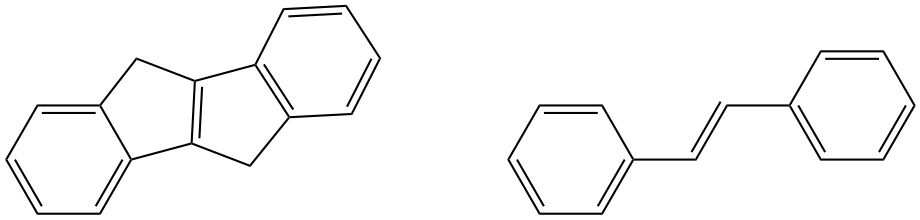
\includegraphics[width=0.6\linewidth]{images/stilbeneindene} 

}

\caption{5,10-dihydroindeno[2,1-a]indene (left) and trans-stilbene (right)}\label{fig:stilbeneindene}
\end{figure}

\hypertarget{sec:SSQemissionans}{%
\section{Self Assessment Question Brief Answers}\label{sec:SSQemissionans}}

\begin{enumerate}
\def\labelenumi{\arabic{enumi}.}
\tightlist
\item
  Absorption occurs almost entirely from the ground vibrational, \(v = 0\), state of the ground electronic state because at room temperature the proportion of the molecules in the \(v = 1\) state is very very low. Molecules are excited into a number of different vibrational levels in the first electronic excited state, the population in each depends upon the overlap integral of the vibrational levels of the ground and excited state.
\end{enumerate}

According to Kasha's rule, emission always happens from the lowest vibrational state, \(v’ = 0\), of the electronically excited state. Emission then happens to all the available vibrational states in the ground electronic state. Absorption transitions from \(v = 0\) to \(v’ = 0\) are lower in energy than transitions from \(v = 0\) to \(v’ = 2\), however emission transitions from \(v’ = 0\) to \(v = 0\) are higher in energy than those from \(v’ = 0\) to \(v = 2\). If were were to sketch these then the two spectra appear as mirror images of each other.

\begin{enumerate}
\def\labelenumi{\arabic{enumi}.}
\setcounter{enumi}{1}
\item
  This is due to Stokes' shift. Absorption occurs from an optimised ground state into an non optimised excited state, this excited state then has time to relax to an optimised configuration before emission of a photon, but by optimising the excited state it destabilises the ground state. Consequently the energy gap between the ground and excited state for absorption is bigger than for emission. Since energy and wavelength are inversely proportional the wavelength of emission is always longer than the wavelength of absorption.
\item
  There is a large energy gap between the \(S_2\) \& \(S_1\) excited states which reduces the efficiency of internal conversion. Given no other deactivation pathway azulene will fluoresce from the \(S_2\) state.
\item
  In the vapour phase, anthracene molecules do not experience the strong and fluctuating interactions with solvent molecules that occur in a solution phase. The vibrational structure is therefore well-defined. The molecules can also rotate giving rise to rotational fine structure in the spectra.
\item
  Internal conversion
  \begin{equation}
  \phi_ic = \frac{k_ic}{k_f^0+k_{ic}+ k_{ST}+k_{\textrm{other}}}
  \label{eq:QYIC}
  \end{equation}
\end{enumerate}

Intersystem crossing (\(S_1\) - \(T_1\))\\
\begin{equation}
\phi_ST = \frac{k_ST}{k_f^0+k_{ic}+ k_{ST}+k_{\textrm{other}}}
\label{eq:QYST}
\end{equation}

Intersystem crossing (\(T_1\) - \(S_0\))\\
\begin{equation}
\phi_TS = \frac{k_TS}{k_f^0+k_{ic}+ k_{ST}+k_{\textrm{other}}}
\label{eq:QYTS}
\end{equation}

\begin{enumerate}
\def\labelenumi{\arabic{enumi}.}
\setcounter{enumi}{5}
\item
  As you work down the halides the amount of spin orbit coupling increases due to the heavy atom effect and the spin selection rules are softened. This leads to a large (nearly x1000) increase in the rate of triplet formation from intersystem crossing. The ratio k\textsubscript{p} / k\textsubscript{ST} changes far less dramatically (0.11, 0.35, 0.32, 0.27, \& 0.38 respectively), this has less to do with the heavy atom effect as it increases both the rate of phosphorescence and singlet to triplet intersystem crossing.
\item
  Essentially the chromophore of stilbene and indene are the same, however stilbene allows rotation of the benzene rings around a single bond allowing efficient internal conversion, whereas the additional structure in the indene does not allow rotational relaxation. With no easy route of internal conversion the quantum yield of fluorescence increases dramatically.
\end{enumerate}

As the sample is cooled the rotation in stilbene is restricted and therefore decreases the rate of internal conversion. As the rate constant for internal conversion decreases then the quantum yield of emission increases as in equation \eqref{eq:QYfluor}.

\hypertarget{ch:Quench}{%
\chapter{Quenching of the Excited State}\label{ch:Quench}}

\hypertarget{sec:QuenchLOs}{%
\subsection{Learning Objectives}\label{sec:QuenchLOs}}

At the end of this section you should be able to:

\begin{itemize}
\tightlist
\item
  Understand the difference between static and dynamic quenching.
\item
  Graphically determine quenching constants for static, dynamic and mixed method quenching.
\item
  Describe mathematically the effect of quenching on emission quantum yields and lifetime.
\item
  Describe the mechanisms of non-collisional energy transfer.
\item
  Demonstrate understanding of the factors which affect the rates of non-collisional energy transfer.
\end{itemize}

\hypertarget{sec:Collisional}{%
\section{Collisional Deactivation of the Excited State}\label{sec:Collisional}}

The photophysical deactivation pathways described above (emission, internal conversion and intersystem crossing) are not the only ways to deactivate an excited state of a molecule, and you perhaps have already noted the use of kother in equations \eqref{eq:QYfluor} - \eqref{eq:QYphos}. Another common pathway of deactivation, particularly in the solution phase, is collisional deactivation commonly known as quenching.

Table \ref{tab:phototrans}, part of which is repeated below, details all of the possible decay pathways from an excited state. Quenching competes with other processes, and consequently reduces the lifetime and yield of emission processes.

\begin{longtable}[]{@{}
  >{\raggedright\arraybackslash}p{(\columnwidth - 2\tabcolsep) * \real{0.6000}}
  >{\raggedright\arraybackslash}p{(\columnwidth - 2\tabcolsep) * \real{0.4000}}@{}}
\toprule
\endhead
\emph{Other pathways} & \\
Quenching of excited state & \(S_1 + Q \longrightarrow S_0 + Q +heat\) \(S_1 + Q \longrightarrow S_0 + Q^\ast +heat\) \(T_1 + Q \longrightarrow S_0 + Q +heat\) \(T_1 + Q \longrightarrow S_0 + Q^\ast +heat\) \\
\bottomrule
\end{longtable}

Quenching of the excited state competes with emission from the excited state, consequently reducing the quantum yield of fluorescence (or phosphorescence).

This bi-molecular, second order quenching process follows Stern-Volmer kinetics, equation \eqref{eq:SternVolmer}, a derivation of which can be found in Wardle, p 88-90).

\begin{equation}
\frac{I_0}{I}=1 + k_q \tau _0 [Q]
\label{eq:SternVolmer}
\end{equation}

Where \(I_0 / I\) is the ratio of the unquenched and quenched steady state intensity of the emission. For dynamic quenching this value will also be the same as \(\phi _0 / \phi\) and \(\tau _0 / \tau\), the ratios of the quantum yield and lifetime respectively, equation \eqref{eq:SternVolmerdynamic}.

\begin{equation}
\frac{I_0}{I}=\frac{\phi_0}{\phi}=\frac{\tau_0}{\tau}=1 + k_q \tau _0 [Q]
\label{eq:SternVolmerdynamic}
\end{equation}

Since this is a second order term when it appears in the equations \eqref{eq:QYfluor} - \eqref{eq:QYphos}, it appears as \(k_q[Q]\), such as indicated in equation \eqref{eq:QYfluorquench}.

\begin{equation}
\phi_f = \frac{k_f^0}{k_f^0+k_{ic}+ k_{ST}+k_q[Q]}
\label{eq:QYfluorquench}
\end{equation}

It is often useful to know if the quenching is diffusion or activation controlled, reactions in the solution phase cannot occur faster than the diffusion controlled rate, with second order rate constant \(k_d\), as described in equation 19.

\begin{equation}
k_d = \frac{8RT}{3 \eta}
\label{eq:diffcontrol}
\end{equation}

where T is the absolute temperature, and η the viscosity of the solvent. (It should be noted that there is an issue with units here where a conversion from m\textsuperscript{3} to dm\textsuperscript{3} is required). Diffusion controlled rates in aqueous, methanol and ethanol solutions are normally in the order of 10\textsuperscript{10} mol\textsuperscript{−1} dm\textsuperscript{3}. Values of rate constant lower than this are termed as activation controlled as only a fraction of the collisions result in a quenching of the excited state of the molecule.

\hypertarget{sec:static}{%
\section{Static Quenching}\label{sec:static}}

Dynamic quenching effects the lifetime of the excited state, as described in equation \eqref{eq:SternVolmerdynamic}. However this is not the case for static quenching; in static quenching an equilibrium exists between dye bound to the quencher and unbound dye and quencher as described below, with equilibrium constant \(K_q\).

\begin{equation*}
\textrm{dye}^\ast \textrm{ + quencher} \rightleftharpoons \textrm{dye:quencher}^\ast
\end{equation*}

\begin{equation*}
K_q = \frac{[\textrm{dye:quencher}]}{[\textrm{dye}][\textrm{quencher}]} 
\end{equation*}

In this case free dye is emissive with an unquenched lifetime, and dye that exists in complex with the quencher is completely non-emissive. Static quenching follows a very similar form to Stern-Volmer as described above, and again a full derivation may be found in Wardle.

\begin{equation}
\frac{I_0}{I}=1 + K_s [Q]
\label{eq:SternVolmerstatic}
\end{equation}

As with dynamic quenching the change in steady state emission is reflected in the change in quantum yield of fluorescence, but this time because the dye exists in either a quenched ( completely non fluorescent) or unquenched (fluorescent) state then the fluorescent lifetime is unchanged in static quenching.

In some cases a quencher can act as both a static and dynamic quencher; in this case the lifetime is only affected from the dynamic quenching and so the rate constant may easily be determined, from knowing this it is simple to determine the equilibrium constant. Systems where there is a combination of static and dynamic quenching are easy to spot as plots of \(I_0 / I\) against the \([Q]\) are curved.

\hypertarget{sec:forster}{%
\section{Förster Resonance Energy Transfer}\label{sec:forster}}

In addition to static and dynamic quenching, as described above, where the excited state of the dye molecule is lost as heat, it is possible for a dye to be quenched by transferring the energy between two chromophores. There are two distinct mechanisms for this happening the first of which is described here; Förster Resonance Energy Transfer (FRET).

\begin{figure}

{\centering 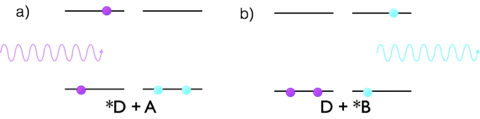
\includegraphics[width=0.7\linewidth]{images/forster} 

}

\caption{The mechanism of Förster resonance energy transfer. a) A donor molecule (purple) is excited by absorption of a photon into an excited state, there is a dipole dipole interaction with the acceptor molecule (blue) which is initially in the ground state. b) the product of energy transfer with the acceptor now in an excited state which is now capable of emission of a photon of lower energy.}\label{fig:forster}
\end{figure}

The first thing to note is that FRET is not a collisional process, energy is transferred between a donor and acceptor moiety at a distance, nor is this an emission of a photon by the donor and reabsorption of this photon by the acceptor.

FRET is a dipole dipole interaction where the acceptor quenches the excited state of the donor by energy transfer between the two moieties, figure \ref{fig:forster}, leaving the donor in an excited state which then decays as described in the a chapter on emission. This dipole-dipole interaction is a co-alligning of the transition dipole moments (see page Section @ref(\#sec:transdipole) on the donor and acceptor molecules - this gives a large dependence on the orientation factors of these two dipoles, the term κ in equation \eqref{eq:rateelectron}. In order for there to be an energy transfer there has to be an overlap between the emission spectra of the donor and the absorption spectra of the acceptor (equation \eqref{eq:overlap}), the greater, as illustrated in figure \ref{fig:overlapintegral}; this is in effect the overlap between the wave function of the excited state donor and the wave function of the ground state donor. The greater this overlap the more efficient the the energy transfer.

\begin{figure}

{\centering 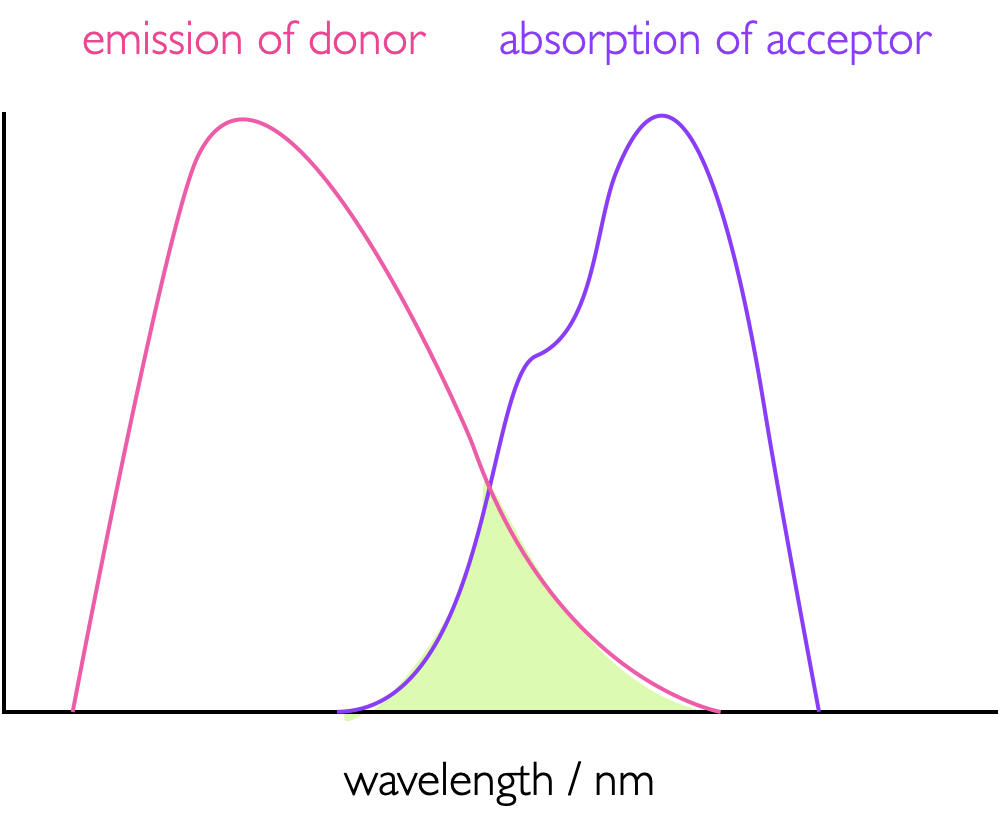
\includegraphics[width=0.7\linewidth]{images/overlapintegral} 

}

\caption{The overlap integral, J, (green shaded area) between the emission spectrum of a donor and absorption spectrum of an acceptor as used in FRET, the greater this overlap integral more more efficient the energy transfer.}\label{fig:overlapintegral}
\end{figure}

\begin{equation}
J (\bar \nu) = \int_0^\infty I_D(\bar \nu)\varepsilon_A(\bar \nu)\textrm{d}\bar \nu
\label{eq:overlap}
\end{equation}

The rate of Förster resonance energy transfer has been found empirically to depend upon a number of factors in addition to the overlap integral, \(J\), such as refractive index of the solvent, \(n\), and the dipole orientation factor \(\kappa\) (equation \eqref{eq:rateelectron}). Perhaps more obviously it also depends upon the separation of donor and acceptor, \(r\), quantum yield of emission of the donor, \(\phi_D\), and the unquenched lifetime of the donor molecule, \(\tau_D\).

\begin{equation}
k_{ET}= \frac{\phi_D \kappa^2}{\tau_D r^6}\frac{9 \ln 10 e^4}{128 \pi^5 N_A n^4}J
\label{eq:rateelectron}
\end{equation}

However, equation \eqref{eq:rateelectron}, is not simple to use, nor particularly descriptive and a simplified version of the equation tends to be used which has defined a `Förster radius', \(R_0\), equations 23 \& 24. The Förster radius is the radius at which half of the emission is quenched by the acceptor.

\begin{equation}
R_0^6=\frac{9 \ln 10 e^4 \phi_D \kappa^2}{128 \pi^5 N_A n^4 }J
\label{eq:forsterdistance}
\end{equation}

\begin{equation}
k_{ET}=\frac{1}{\tau_D}\frac{R_0^6}{r^6}
\label{eq:forstersimplified}
\end{equation}

Förster distances tend to be between 20 - 90 Å, and due to the parity of this with the size of biological macromolecules FRET is an excellent technique for studying biomolecules.
The quantum yield of Förster energy transfer, \(Φ_{ET}\) (equation \eqref{eq:QYET}), is usually just given the symbol \(E\), for efficiency. As described in equations \eqref{eq:rateelectron} - \eqref{eq:forstersimplified} this can be defined by:

\begin{equation}
\phi_ET = \frac{k_ET}{k_f^0+k_{ic}+ k_{ST}+k_{ET}}
\label{eq:QYET}
\end{equation}

By combining equations \eqref{eq:forstersimplified} \& \eqref{eq:QYET} it becomes easy to see how the efficiency of Förster energy transfer (\(E\) or \(Φ_{ET}\)) depends upon the distance, and we can see that the efficiency of energy transfer is 0.5 at the Förster distance. Figure \ref{fig:forsterdistance} sketches the distance dependence of efficiency of energy transfer, where it can be seen that at twice the Förster distance the efficiency has dropped almost to 0.

\begin{figure}

{\centering 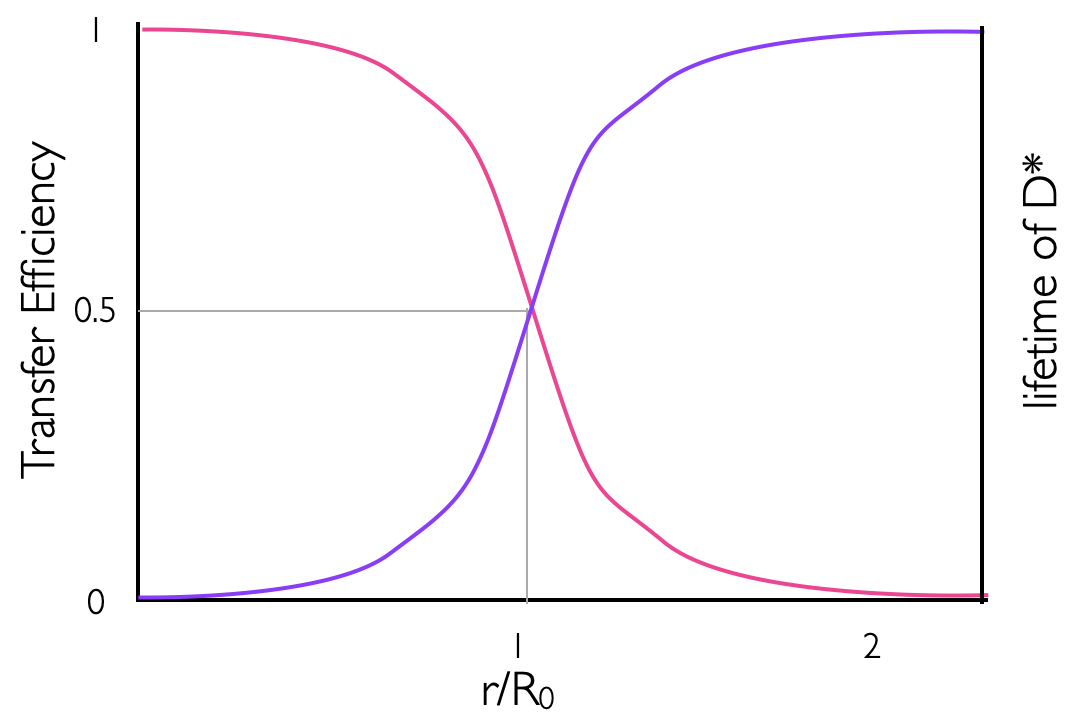
\includegraphics[width=0.7\linewidth]{images/forsterdistance} 

}

\caption{The distance dependence on the efficiency of energy transfer between a donor and acceptor in Förster resonance energy transfer (pink line), the purple line represents the distance dependence variation in the measured lifetime of the donor molecule with a maximum value of the unquenched donor of τ~D~..}\label{fig:forsterdistance}
\end{figure}

\begin{equation}
E=1-\frac{\tau_{DA}}{\tau_D}
\label{eq:efflifetime}
\end{equation}

\begin{equation}
E = \frac{R_0^6}{R_0^6+ r^6}
\label{eq:effdistance}
\end{equation}

The efficiency of energy transfer is calculated by measuring the quenched and unquenched fluorescence lifetime of the donor molecule. More detailed derivations of equations \eqref{eq:efflifetime} \& \eqref{eq:effdistance} may be found in Turro, Principles of Molecular Photochemistry.

Experimentally the process is confirmed to energy transfer at a distance, and not collisional energy transfer, as the rate constant of energy transfer \(k_{ET}\) is independent of solvent viscosity (as seen in equation \eqref{eq:diffcontrol} \& Stern-Volmer kinetics) and rates can be significantly higher than the rate limiting diffusion controlled rates. The energy is transferred by a dipole-dipole interaction.

\hypertarget{sec:Dexter}{%
\section{Dexter Energy Transfer}\label{sec:Dexter}}

Forster resonance energy transfer transfers energy between a donor an acceptor moiety by a dipole dipole interaction, however there is a second method of energy transfer which takes place by a slightly different mechanism. Dexter energy transfer transfers energy from a donor to acceptor moiety by a concerted exchange of electrons between the chromophores, figure \ref{fig:Dexter}.

\begin{figure}

{\centering 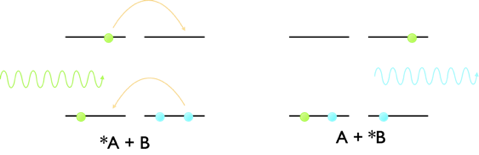
\includegraphics[width=0.7\linewidth]{images/Dexter} 

}

\caption{ The mechanism of Dexter energy transfer, where there is a concerted exchange of electrons from the LUMO of the donor to the empty LUMO of the acceptor and at the same time from the HOMO of the acceptor to the HOMO of donor. The two electrons move at the same time leading to a net exchange of energy from the donor to acceptor.}\label{fig:Dexter}
\end{figure}

The rate of Dexter energy transfer is again distance dependent and again is dependent upon the overlap integral, J, between the emission of the donor and the absorption of the acceptor (figure \ref{fig:overlapintegral}, equation \eqref{eq:overlap}). The rate of Dexter energy transfer is given by:

\begin{equation}
k_{ET}=KJe^{-\frac{2r}{L}}
\label{eq:ratedexter}
\end{equation}

where \(J\) is the overlap integral, \(K\) an empirical constant, \(r\) the separation between the donor and acceptor, and \(L\) another constant which represents the closest possible separation of the donor and acceptor (the sum of the van der Waals radii of the two chromophores).

From examining equation \eqref{eq:ratedexter} it can be seen that the rate of Dexter energy transfer decreases rapidly with increasing separation of donor and acceptor and occurs daily at distances less than 20 Å. Dexter energy transfer is the most dominant mechanism of triplet-triplet quenching.

\hypertarget{sec:tripletannihilation}{%
\section{Triplet-Triplet Annihilation}\label{sec:tripletannihilation}}

Excited state triplets are long lived, due to the spin-forbidden relaxation pathways back to the \(S_0\) state. However, there is a deactivation pathway that occurs by annihilation of two triplet states leading to formation of an excited state singlet and a ground state singlet.

\begin{figure}

{\centering 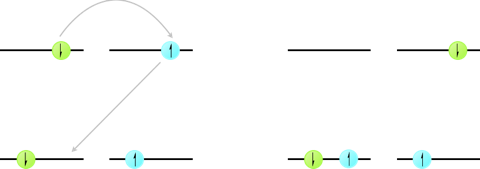
\includegraphics[width=0.7\linewidth]{images/triplettriplet} 

}

\caption{The mechanism of triplet triplet annihilation by Dexter energy transfer, concerted electron exchange between a donor and acceptor molecule leading to formation of a singlet excited state on one molecule and a ground state singlet on the other molecule.}\label{fig:triplettriplet}
\end{figure}

\begin{equation*}
^\ast D_{T_1}+^\ast D_{T_1} \longrightarrow ^\ast D_{S_1} + D_{S_0}
\end{equation*}

Triplet-triplet annihilation is the reason that quantum yields of phosphorescence are almost never unity (1).

\hypertarget{sec:O2quench}{%
\section{Quenching by Molecular Oxygen}\label{sec:O2quench}}

\begin{figure}

{\centering 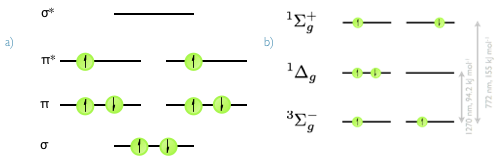
\includegraphics[width=0.7\linewidth]{images/O2} 

}

\caption{a) The valence set of molecular orbitals in molecular oxygen, showing the full electronic arrangement for the 3Σg− triplet ground state.  b) The π* HOMO orbital of molecular oxygen, with the 3Σg− triplet ground state and the singlet excited states 1Δg and 1Σg+.The relative energies of the two excited states are indicated.}\label{fig:O2}
\end{figure}

Molecular oxygen is unusual because it is a ground state triplet. It is an efficient quencher of excited triplet states because it has two accessible excited singlet states, figure \ref{fig:O2}. It is also capable of quenching excited singlet states, however since the quenching occurs by a Dexter mechanism the overlap integral between excited singlet states and ground state molecular oxygen tends to be very small leading to very small quantum yields of singlet oxygen formation.

\begin{equation}
\textrm{O}_2(^3 \Sigma _g^-)+ ^\ast \textrm{Dye}(T_1) \longrightarrow ^\ast \textrm{O}_2(^1 \Delta _g) + \textrm{Dye}(S_0)
\label{eq:O2quench}
\end{equation}

Usually the molecular oxygen is excited into the \^{}\textsuperscript{Σ\textsubscript{g}}+\^{} state, but this rapidly decays to the \textsuperscript{1}Δ\textsubscript{g} state. The \textsuperscript{1}Δ\textsubscript{g} is usually simply referred to as singlet oxygen and is relatively stable because of the spin forbidden deactivation, having a lifetime of a few µs in aqueous solvent and hours in the gas phase.

Chemically singlet oxygen formation is very interesting as it is extremely reactive, and has been shown to be an important factor in a number of mechanistic pathways leading to damage of DNA and proteins.

\hypertarget{before-completing-this-section-1}{%
\section{Before Completing this Section}\label{before-completing-this-section-1}}

To support the material in this section it is suggested you read chapter 6 of Wardle `Principles and Application of Photochemistry'.

\hypertarget{sec:SAQquench}{%
\section{Self Assessment Questions}\label{sec:SAQquench}}

\begin{enumerate}
\def\labelenumi{\arabic{enumi}.}
\tightlist
\item
  Sketch suitable graphs to determine:

  \begin{itemize}
  \tightlist
  \item
    the rate constant of quenching of a dynamically quenched system and
  \item
    the equilibrium (binding) constant of a statically quenched system.
  \end{itemize}
\end{enumerate}

\begin{itemize}
\tightlist
\item
  How will these constants vary with increasing temperature in each case?
\end{itemize}

\begin{enumerate}
\def\labelenumi{\arabic{enumi}.}
\setcounter{enumi}{1}
\item
  Draw a molecular orbital diagram of ground state molecular oxygen, and show how oxygen can behave as a quencher by energy transfer. Why is the quenching by molecular oxygen of singlet states not efficient?
\item
  A donor, D, with an unquenched lifetime of 5.0 ns, was found to have a steady state emission intensity of 20.5 in free solution and 4.1 when in the presence of a quencher, Q. Assuming the Förster distance is 50 Å determine :

  \begin{itemize}
  \tightlist
  \item
    the transfer efficiency, E.
  \item
    the lifetime of D in the presence of the quencher Q
  \item
    the equilibrium separation of D \& Q
  \item
    the rate constant for energy transfer
  \end{itemize}
\end{enumerate}

\hypertarget{sec:SAQquenchans}{%
\section{Self Assessment Question Brief Answers}\label{sec:SAQquenchans}}

\begin{enumerate}
\def\labelenumi{\arabic{enumi}.}
\tightlist
\item
  For the dynamically quenched system, increasing the temperature will increase the number of collisions and so the dynamic rate constant will increase, however, for the statically quenched system increasing the temperature will almost certainly drive the equilibrium towards the unbound system decreasing the observed quenching upon increasing the temperature.
\end{enumerate}

\begin{figure}

{\centering 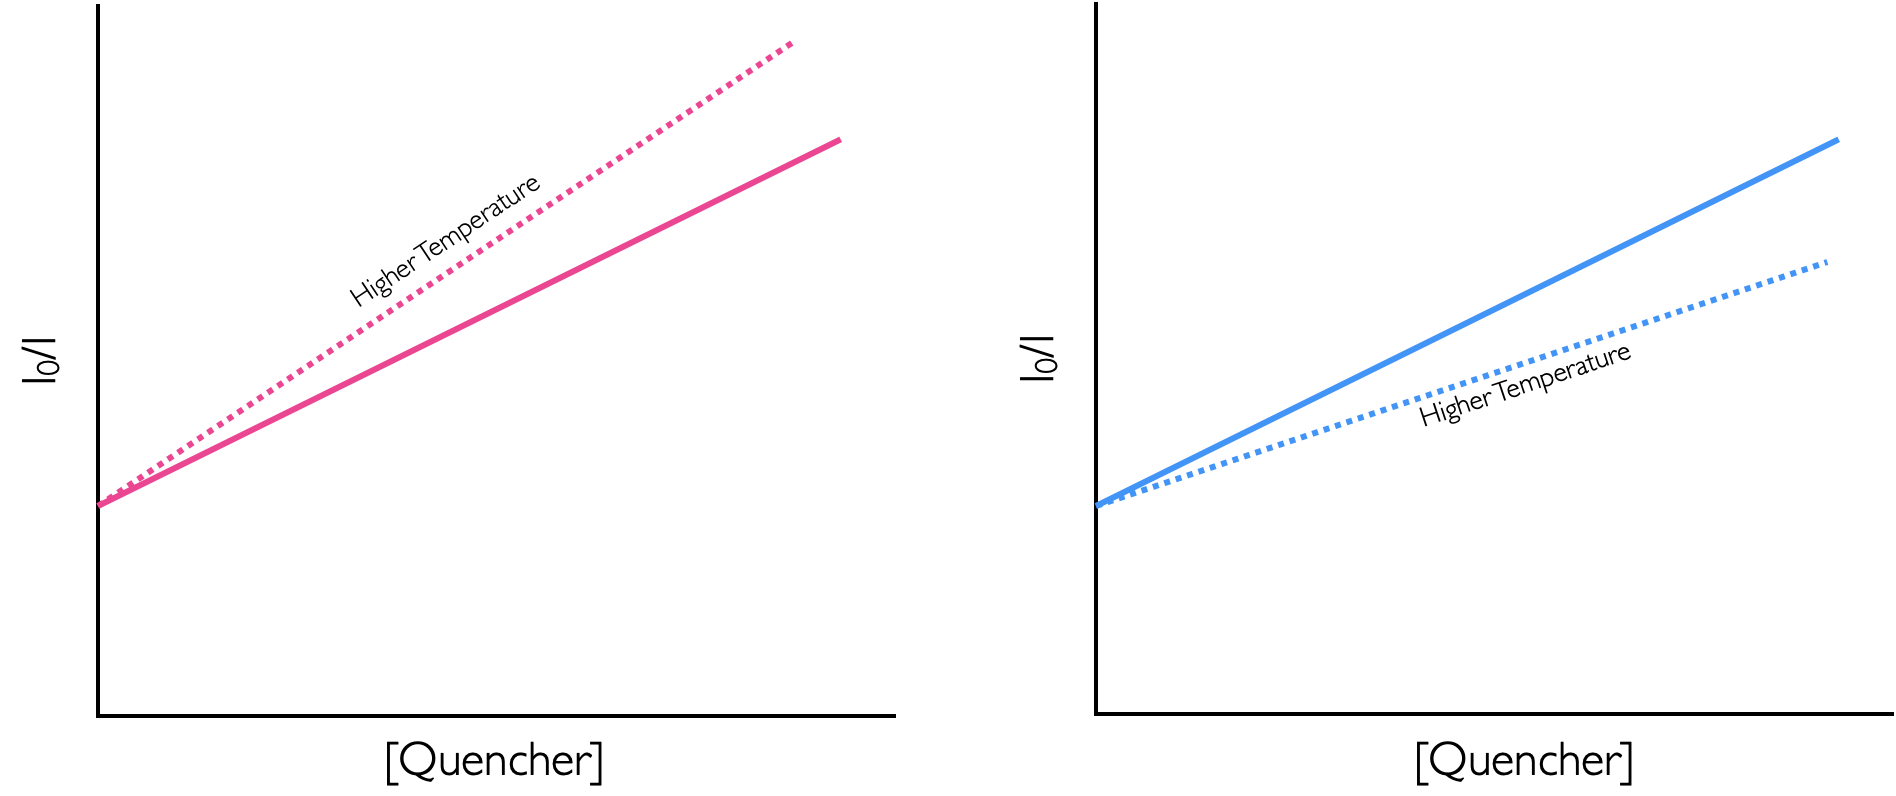
\includegraphics[width=0.7\linewidth]{images/quenchintensityconc} 

}

\caption{The effect of tempearture on the quenching efficiency of dynamic (pink on the left) and static (green on the right) quenching}\label{fig:quenchintensityconc}
\end{figure}

\begin{enumerate}
\def\labelenumi{\arabic{enumi}.}
\setcounter{enumi}{1}
\item
  The energy level diagram for molecular oxygen may be found in figure \ref{fig:O2}.

  Singlet states only have a short lifetime and so quenching is less efficient due to the limitation of diffusion occurring within the lifetime of the excited state, and the overlap integral are much lower between singlet and triplet states due in part to the higher energy of the singlet state (recall there needs to be an overlap of the emission spectrum of the donor and absorption spectrum of the quencher for energy transfer).

  The energy transfer for triplet quenching, is almost certainly by the Dexter mechanism, with the sensitiser going from an excited triplet state (T\textsubscript{1}) to the ground singlet state (S\textsubscript{0}).
\end{enumerate}

\begin{figure}

{\centering 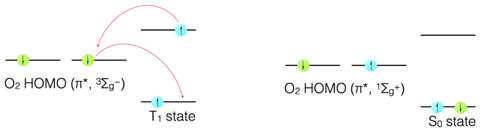
\includegraphics[width=0.7\linewidth]{images/O2quench} 

}

\caption{Dexter mechanism of energy transfer from a triplet excited state and ground state molecular oxygen.}\label{fig:O2quench}
\end{figure}

\begin{enumerate}
\def\labelenumi{\arabic{enumi}.}
\setcounter{enumi}{2}
\item
  The steady state intensity may also be used to determine the efficiency as it is a measure of how much the system is quenched, just like with dynamic Stern Volmer kinetics, hence:

  \begin{itemize}
  \tightlist
  \item
    \(E = 1 − \frac{I_{DQ}}{I_D}\)
  \end{itemize}

  \(E = 1 − \frac{4.1}{20.5}\)

  \(E = 0.8\)

  \begin{itemize}
  \item
    \(E = 1 − \tau_{DQ} / \tau_D\)
    \(\tau_{DQ} = 1.0\) ns
  \item
    Using equation \eqref{eq:effdistance} \(r = 38.2\) Å
  \item
    Using equation \eqref{eq:forstersimplified} \(k_{ET} = 8 × 10^8\) s\textsuperscript{−1}
  \end{itemize}
\end{enumerate}

\hypertarget{ch:excited}{%
\chapter{Other Excited State Systems}\label{ch:excited}}

\hypertarget{sec:exitedLOs}{%
\subsection{Learning Objectives}\label{sec:exitedLOs}}

At the end of this section you should be able to:

\begin{itemize}
\tightlist
\item
  Explain the origin of excimer and exciplex emission spectra.
\item
  Describe why excimer and exciplex formation are concentration dependent.
\item
  Interpret changes in emission spectra with changing concentration to justify formation of either excimers or exciplexes.
\end{itemize}

\hypertarget{sec:excimers}{%
\section{Excimers}\label{sec:excimers}}

An excimer is an excited state dimer formed between two identical molecules. A photon is delocalised between two molecules which in the excited state are weakly bound together. Excimers are relatively long lived species, and were first noticed when increasing the concentration of certain fluorophores.

It was found that upon increasing the concentration of the chromophore the fluorescence did not increase linearly, and upon reaching higher concentrations the fluorescence decreased; however, this decrease in fluorescence occurred with an increase in a new emission band of lower energy. Excimer bands tend to be broad featureless and Gaussian in profile, figure 33. It is important to note that there is no bonding between the chromophores in the ground state; excimers only occur at high concentrations as an excited state molecule has to interact with a second ground state molecule in the lifetime of the excited state. There is no change in the absorption of the sample (as there is only excitation of monomer species), only formation of a new band in the emission spectrum.

Excimers exist because of formation of a weak bond between the two chromophores as shown in figure \ref{fig:excimer}. By formation of this bond any emission from the excimer has to be lower in energy than the fluorescence of the monomer chromophore. The ground state consists of two molecules in an dissociated state, upon emission from the excimer the structure of the excimer remains (as with the Stokes shift) and the two molecules diffuse apart.

It is important to note that there is no charge separation in the excimer and that the excited state is shared across both molecules.

\begin{figure}

{\centering 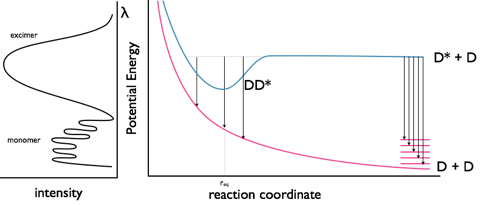
\includegraphics[width=0.7\linewidth]{images/excimer} 

}

\caption{The monomer and excimer emission of pyrene, and an energy level profile showing the fluorescence from the non-bonded D* state as well as the excimer emission from the DD* state.}\label{fig:excimer}
\end{figure}

\begin{figure}

{\centering 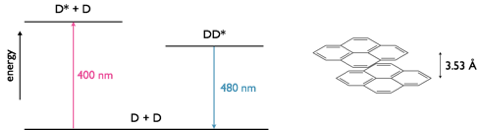
\includegraphics[width=0.7\linewidth]{images/pyreneexcimer} 

}

\caption{A pyrene excimer with a separation of 3.53 Å between the two planes of nuclei, in the excited state dimer the two ring systems of pyrene have a weak interaction between them. The emission maxima of fluorescence is 400 nm whereas the emission maxima for the excimer is 480 nm.}\label{fig:pyreneexcimer}
\end{figure}

A concept bite video briefly covering the concepts of eximers and exciplexes (video length 7m05s)

\hypertarget{exciplexes}{%
\section{Exciplexes}\label{exciplexes}}

Excimers consist of an excited state shared between two identical monomer units, whereas exciplexes are excited state complexes of two different chromophores. Due to the differences in molecular orbitals of the chromophores exciplexes have a dipole across the excited state complex; this dipole can lead to formation of a charge separated species, figure \ref{fig:exciplex}.

Exciplexes can undergo emission from this state, leading to formation of dissociated monomer units or there can be a solvent reorganisation leading to formation of a solvent separated radical ion pair, at this point there can still be charge recombination and relaxation of the system (this time with the excess energy lost as heat) to the original monomer chromophore units.

\begin{figure}

{\centering 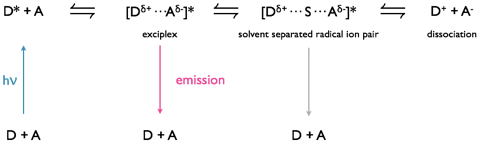
\includegraphics[width=0.7\linewidth]{images/exciplex} 

}

\caption{Formation of an exciplex from an excited state donor and ground state acceptor chromophore. The exciplex has a small charge separation leading to a dipole over the excited state complex, under some circumstances with the introduction of solvent between the chromophores in the exciplex this can then go on to form a solvent separated radical ion pair which may then go on to form a charge separated redox pair.}\label{fig:exciplex}
\end{figure}

\begin{figure}

{\centering 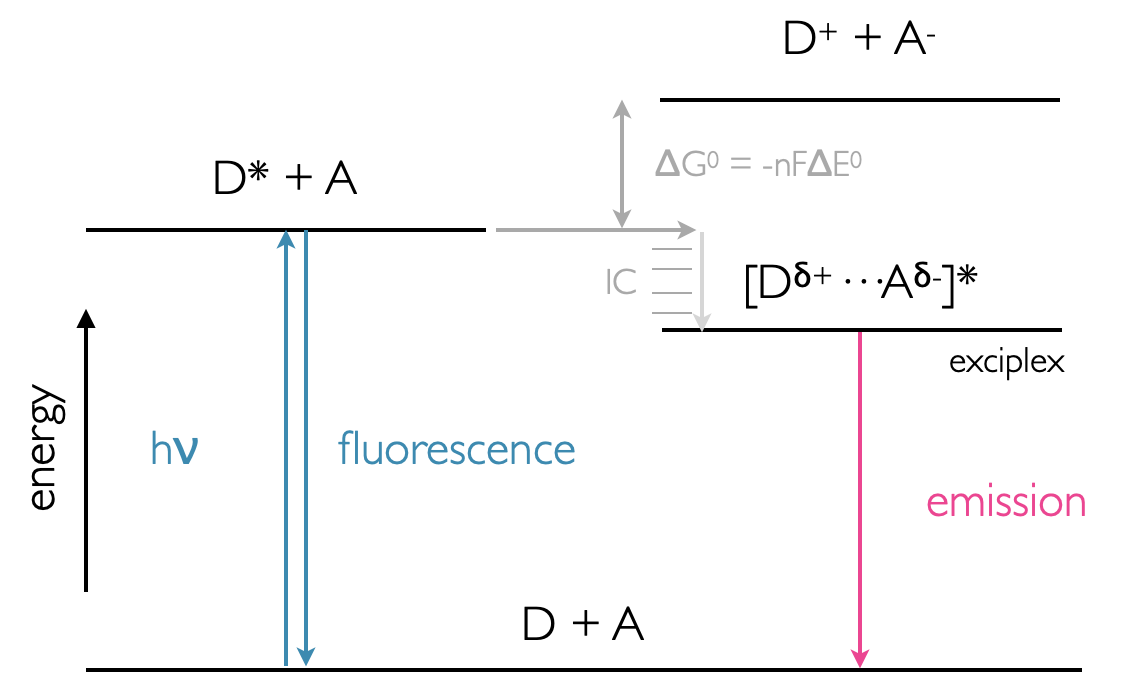
\includegraphics[width=0.7\linewidth]{images/exciplexenergy} 

}

\caption{Energy profile of exciplex formation showing the lower energy state of the exciplex over the D* + A system. Emission from the exciplex is lower energy than fluorescence from the monomer donor chromophore.}\label{fig:exciplexenergy}
\end{figure}

Exciplexes are common in organic solvent as non polar solvents are not good at stabilising ions in solution, as the polarity of the solvent increases then the charge separated state becomes more favoured. Exciplexes and other charge separated species are of interest in chemistry for use in molecular wires and energy storage devices.

Please see video above in Section \ref{sec:excimers} for a review of this topic (timecode 4m52s).

\hypertarget{before-completing-this-section-2}{%
\section{Before Completing this Section}\label{before-completing-this-section-2}}

To support the material in this section it is suggested you read pages 90-96 of Wardle `Principles and Application of Photochemistry'.

\hypertarget{self-assessment-questions}{%
\section{Self Assessment Questions}\label{self-assessment-questions}}

\begin{enumerate}
\def\labelenumi{\arabic{enumi}.}
\tightlist
\item
  Low concentration solutions of pyrene in ethanol have a characteristic violet fluorescence emission (spectrum labeled 4), however upon increasing the concentration this emission becomes sky blue (spectra 3,2,1 as increasing concentration of pyrene). Explain the origin of this shift and also the changing characteristic of the emission spectrum.
\end{enumerate}

\begin{figure}

{\centering 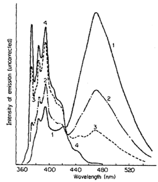
\includegraphics[width=0.7\linewidth]{images/pyrenespec} 

}

\caption{Question 1. Pyrene spectrum in ethanol at different concentrations.}\label{fig:pyrenespec}
\end{figure}

\begin{enumerate}
\def\labelenumi{\arabic{enumi}.}
\setcounter{enumi}{1}
\tightlist
\item
  The fluorescence emission from anthracene in dry toluene is violet (spectrum 1), however upon addition of diethylaniline (2,3,4 are increasing concentrations respectively) the emission becomes greener. Explain the change in the colour of emission and the change in the shape of the emission spectra.
\end{enumerate}

\begin{figure}

{\centering 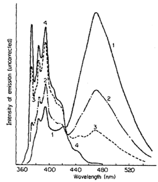
\includegraphics[width=0.7\linewidth]{images/pyrenespec} 

}

\caption{Question 2. Anthracene spectrum in dry toluene at different concentrations.}\label{fig:anthracenespec}
\end{figure}

\hypertarget{self-assessment-question-brief-answers}{%
\section{Self Assessment Question Brief Answers}\label{self-assessment-question-brief-answers}}

\begin{enumerate}
\def\labelenumi{\arabic{enumi}.}
\item
  At low concentrations the maximum emission occurs around 400 nm, with very little emission at wavelengths longer than 440 nm, this accounts for the violet emission. At higher concentrations a symmetric (gaussian profile) band is seen to grow in centred around 480 nm (blue) with a decreasing monomer emission between 360 \& 440 nm. The lack of structure and the increasing in intensity of this band with increasing concentration of chromophore indicates the presence of a excimer emission from an excited state pyrene dimer. The fine structure in the monomer band is due to relaxation from the \(S_1\), v' = 0 lowest energy vibrational state of the excited state to a variety of vibrational levels in the ground state, v = 0, 1, 2, 3\ldots{} with the highest energy emission \textasciitilde{} 375 nm accounting for the \(S_1\) v' = 0 → \(S_0\) v = 0 state, with the next peak around 385 nm \(S_1\) v' = 0 → \(S_0\) v = 1 transition, \emph{etc}. The Gaussian band is lower in energy than the monomer emission due to the stabilisation of dimerising in the excimer complex, the lack of structure is due to the ground state of the excimer being the repulsive non-bonding regime (figure \ref{fig:excimer}).
\item
  The spectrum labelled 1, is the monomer emission of anthracene it shows an emission maxima around 410 nm and fine structure due to vibronic transitions from the ground vibrational electronically excited state to vibrationally excited ground electronic state levels (see above), upon addition of diethyl aniline this emission is dramatically quenched and a new band focused around 500~nm appears. This band is highly symmetrical and lower in energy than the monomer emission indicating it is due to emission from an exciplex state, the excited state complex is more common at higher concentrations of diethyl aniline, so the monomer emission decreases as the excimer emission increases.
\end{enumerate}

\hypertarget{photochemistry}{%
\chapter{Photochemistry}\label{photochemistry}}

\hypertarget{sec:photochemLOs}{%
\subsection{Learning Objectives}\label{sec:photochemLOs}}

At the end of this section you should be able to:

\begin{itemize}
\tightlist
\item
  Show an awareness of excited state reactions and rearrangements.
\item
  Discuss energy transfer, excitons and delayed fluorescence.
\item
  Explain pictorially why the rate of some chemical reactions may be slowed upon promotion to a high excited state.
\end{itemize}

There are a number of reactions in which light is an essential component, indeed life on earth wouldn't occur without a photosensitised reaction, nor would we be able to see. This work is little more than an introduction to the fundamental processes, however it should be noted that using light is becoming increasingly important in modern chemistry research. Whether this is for use in sensors, medicine, or energy production the fundamental concepts are largely the same, and these concepts are introduced here.

\hypertarget{sec:photoinducedisom}{%
\section{Photoinduced Isomerisation}\label{sec:photoinducedisom}}

When discussing the absorption of light it was noted that by promotion of an electron into an anti-bonding orbital the bond order was reduced. In the case of double (π) bonds in molecules such as retinal (figure), the bond order of one of the double bonds is reduced and therefore allows rotation around this now single bond, as the energy is lost (either by internal conversion or emission) the π-bond is restored. A simple Lewis model of bonding is convenient, however we have to consider the molecular orbital, and this version of bonding highlights a particular bond which is weakened in the excited state, consequently rotation occurs around a specific bond in a conjugated chain.

\begin{figure}

{\centering 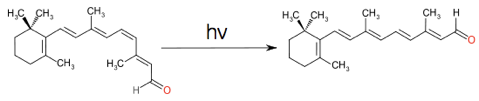
\includegraphics[width=0.7\linewidth]{images/retinal} 

}

\caption{The cis-trans isomerisation of retinal, which when combined with the protein rhodopsin is vital in vision. Absorption of a photon, reduces the bond order of a specific bond due to characteristics of the excited state molecular orbital.}\label{fig:retinal}
\end{figure}

The steady state photochemical yield of any such cis-trans isomerisation will depend upon the absorption of each of the chromophore isomers at the excitation wavelength, the composition of this steady state is referred to as the photostationary state. The composition of this photostationary state may be easily calculated making only minor assumptions.

The most important of these assumptions is that when in the excited state there is an equal probability that the molecule will relax to the cis \& trans states. The second assumption is that (near) monochromatic light is used, because we have already seen that the molar extinction coefficient is very wavelength dependent. Finally the excitation has to occur long enough for the (steady state) photostationary state to be established.

Figure \ref{fig:cistransstilbene} shows the absorption spectra of the two isomers of stilbene, there are a number of interesting photophysical details about this molecule, but it should be noted that the molar extinction coefficient is different for each of the isomers. The point where the two spectra cross is called the isobestic point , for stilbene this is 288 nm, if the system is excited at this wavelength then the yield of each isomer will be the same. However at all other wavelengths the yield of one isomer will be higher than the other. If an excitation wavelength is used whereby the molar extinction coefficient of the trans isomer is highest then this isomer is excited preferentially and there is less of this isomer is the photostationary state.

\begin{figure}

{\centering 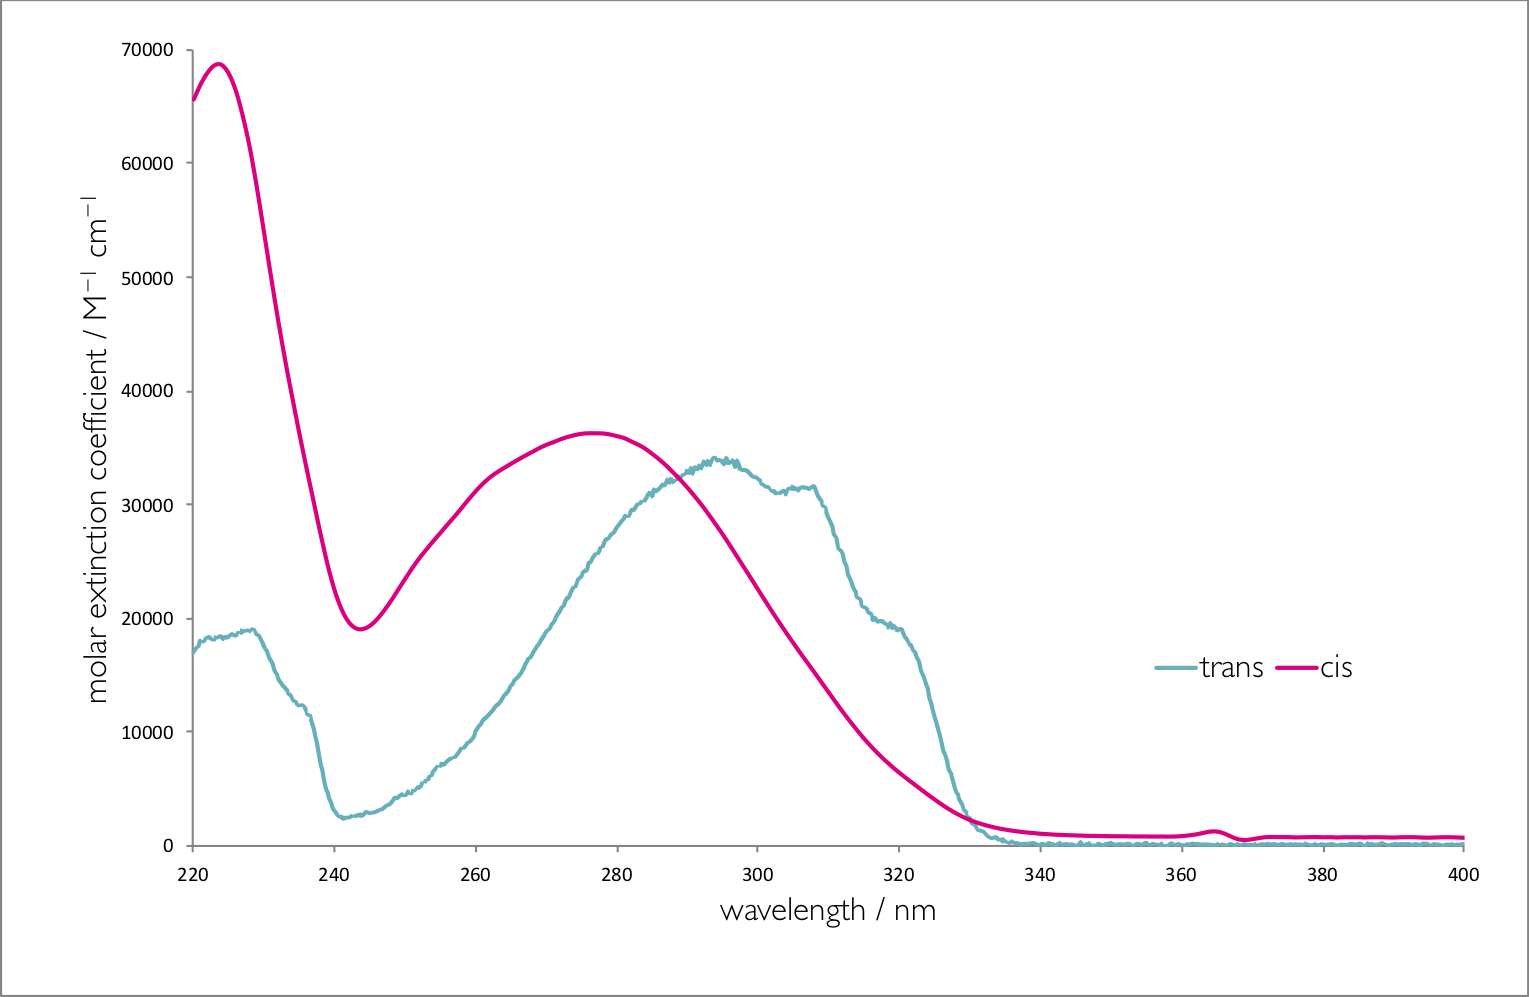
\includegraphics[width=0.6\linewidth]{images/cistransstilbene} 

}

\caption{The absorption spectra of trans and cis stilbene in hexane.}\label{fig:cistransstilbene}
\end{figure}

In summary the higher the molar absorption coefficient at the excitation wavelength the lower the yield of that product in the photostationary state.

The dynamics of cis-trans isomerisation may be studies by using some of the photophysics already discussed. Figure \ref{fig:cisquench} shows a cis / trans system, in the cis position the emission from a fluorophore is quenched so there is no visible emission from the dye. In the trans position position of the quencher now means that there is either no quenching or the quenching is greatly reduced, consequently the emission from the fluorophore is greatly increased.

\begin{figure}

{\centering 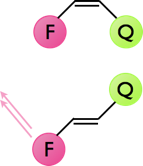
\includegraphics[width=0.2\linewidth]{images/cisquench} 

}

\caption{The quenching of emission of a fluorophore by a nearby quencher, in the cis configuration the emission from the fluorophore is completely quenched, whereas in the trans configuration emission from the fluorophore is observed.}\label{fig:cisquench}
\end{figure}

\hypertarget{sec:photoinducedrearrange}{%
\section{Photoinduced Rearrangements}\label{sec:photoinducedrearrange}}

Cis / trans isomerisations are not the only type of photochemical reaction; dienes, trienes and polyenes often undergo structural isomerisation, specifically cyclisation reactions. Upon excitation 1,3-butadiene undergoes a ring closing reaction to form cyclobutene. This reaction only occurs from the cis isomer, the trans isomer will instead rearrange as described above.

Reactions of polyenes are highly dependent upon the electronic configuration of the excited state with chemistry from singlet states being very different to chemistry from triplet states. The longer lived triplet states frequently undergo second order dimerisation reactions, whereas the singlet states lead to a internal single molecule cyclisation reactions.

Direct absorption of light may only lead to one of the possible products, for systems with a low triplet yield it is not easy to undergo dimerisation reactions, even if this is the desired products. Instead of direct absorption of light, which frequently only leads to the singlet state, a photosensitiser may be used, use of a sensitiser is common for selective reactions of alkenes or aromatic compounds.

A triplet sensitiser may induce a triplet state in another molecule by energy transfer. A sensitiser molecule maybe excited and relax, via intersystem crossing into an excited triplet state. This sensitiser then undergoes an energy transfer reaction with the ground state alkene molecule. Since the sensitiser was in a triplet state the excited state alkene will also be in a triplet state, and now reaction products of the excited state may will be different from products of the singlet excited state.

One thing to note for photosensitised reactions is now the photostationary state yield has nothing to do with the absorption coefficient of either of the states. Consequently if a products has to be isometrically pure a sensitiser is often used to ensure high yields of only one of the photoactive isomers.

\hypertarget{sec:photoinducedelec}{%
\section{Photoinduced Electron Transfer}\label{sec:photoinducedelec}}

Redox reactions are an incredibly important class of chemical reaction with the simplest of these being movement of a single electron from a donor (oxidiser) to an acceptor (reduced). In a redox process we are effectively removing an electron from the HOMO of a donor, to an infinite distance (where there are no charge charge interactions, recall definitions of ionisation energy), and then returning that electron from infinity to the LUMO of an acceptor molecule. Redox reactions have traditionally occurred if you get more energy back from the reduction than it takes to oxidise the donor.

However, if we excite an electron from the HOMO into the LUMO then the energy it takes to oxidise the molecule is reduced. Consequently a molecule in its excited state is a better reducing agent than a molecule in its ground state, and redox reactions that cannot occur from the ground state can occur from the excited state, figure \ref{fig:donoret}.

\begin{figure}

{\centering 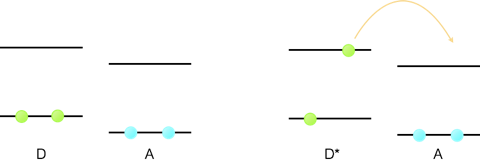
\includegraphics[width=0.6\linewidth]{images/donoret} 

}

\caption{The one electron redox reaction of a donor molecule, D, and acceptor A. For the ground state the empty LUMO is higher in energy than the donor HOMO and so no reaction occurs. Upon excitation of the dye, D*, the donor electron is now higher in energy than the empty LUMO and so the one electron transfer reaction can occur.}\label{fig:donoret}
\end{figure}

This is not the only mechanism by which an excited state can lead to movement of an electron between two molecules. Figure \ref{fig:acceptoret} shows a hole transfer reaction (movement of a vacancy), where by a chromophore is excited and an electron moves from a second molecule into the hole left behind in the HOMO orbital.

\begin{figure}

{\centering 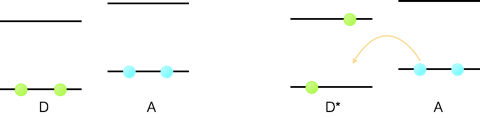
\includegraphics[width=0.6\linewidth]{images/acceptoret} 

}

\caption{A hole transfer reaction, where a molecule is excited an the electron transfers from the ground state HOMO orbital of a second molecule into the vacancy in the HOMO orbital of the excited chromophore.}\label{fig:acceptoret}
\end{figure}

Since the electron moves between the two molecules there has to be an overlap between the molecular orbitals of the donor and acceptor molecules.

The Rehm-Weller equation (equation \eqref{eq:rehmweller}), relates the driving force of a photochemically promoted electron transfer reaction to the redox potentials of the donor (reducing agent Eº(D\textsubscript{•+}/D)) and the acceptor (oxidising agent Eº(A/A\textsubscript{•−}) and the energy gained by promotion of an electron into a LUMO orbital (E\textsubscript{0,0}, quite literally the energy between the ground and excited electronic states for the v=0 bands). There is a small correction factor required, ω(r) but in polar solvents this is negligible, e is the elementary charge on an electron, so in this form this is the driving force for movement of a single electron. This process is normally called photo induced electron transfer.

\begin{equation}
\Delta G ^\circ = e[E^\circ(D^{\bullet +}/D)-]E^\circ(A-A^{\bullet -})]-E_{0,0} + \omega (r)
\label{eq:rehmweller}
\end{equation}

\hypertarget{sec:marcus}{%
\section{Marcus Theory of Electron Transfer}\label{sec:marcus}}

The rates of other mechanisms of excited state reactions have all been detailed in chapter \ref{ch:Quench}, but so far, whilst I have described the mechanisms of electron transfer between a donor and an acceptor we have not quantified the rates of these reactions.

The rate of electron transfer was found to depend upon a number of factors described by the Marcus equation \eqref{eq:marcus}.

\begin{equation}
k_{et}=\frac{2 \pi |V(r)|^2}{h}\frac{1}{\sqrt{4 \pi \lambda k_B T}}e^{-\frac{(\Delta G^\circ+ \lambda)^2}{4 \lambda k_B T}}
\label{eq:marcus}
\end{equation}

where:

\begin{equation}
|V(r)|=|V(r)|^\circ e^{-\frac{\beta(r-r_\circ)}{2}}
\label{eq:coupel}
\end{equation}

At first, and indeed second glance this equation can be overwhelming. There are a number of new terms in this equation, which we will break down further, however what is interesting is that a thermodynamic term (\(\Delta G^\circ\)) appears in our kinetic equations.

If we recall our discussion on Stokes shift (section \ref{sec:stoke} we introduced the idea of reorganisation of both the chromophore and solvent environment upon excitation of an electron from a ground to an excited state. There is a similar reorganisation of both chromophore and solvent upon either one electron oxidation (or reduction), figure \ref{fig:elecreorg}.

\begin{figure}

{\centering 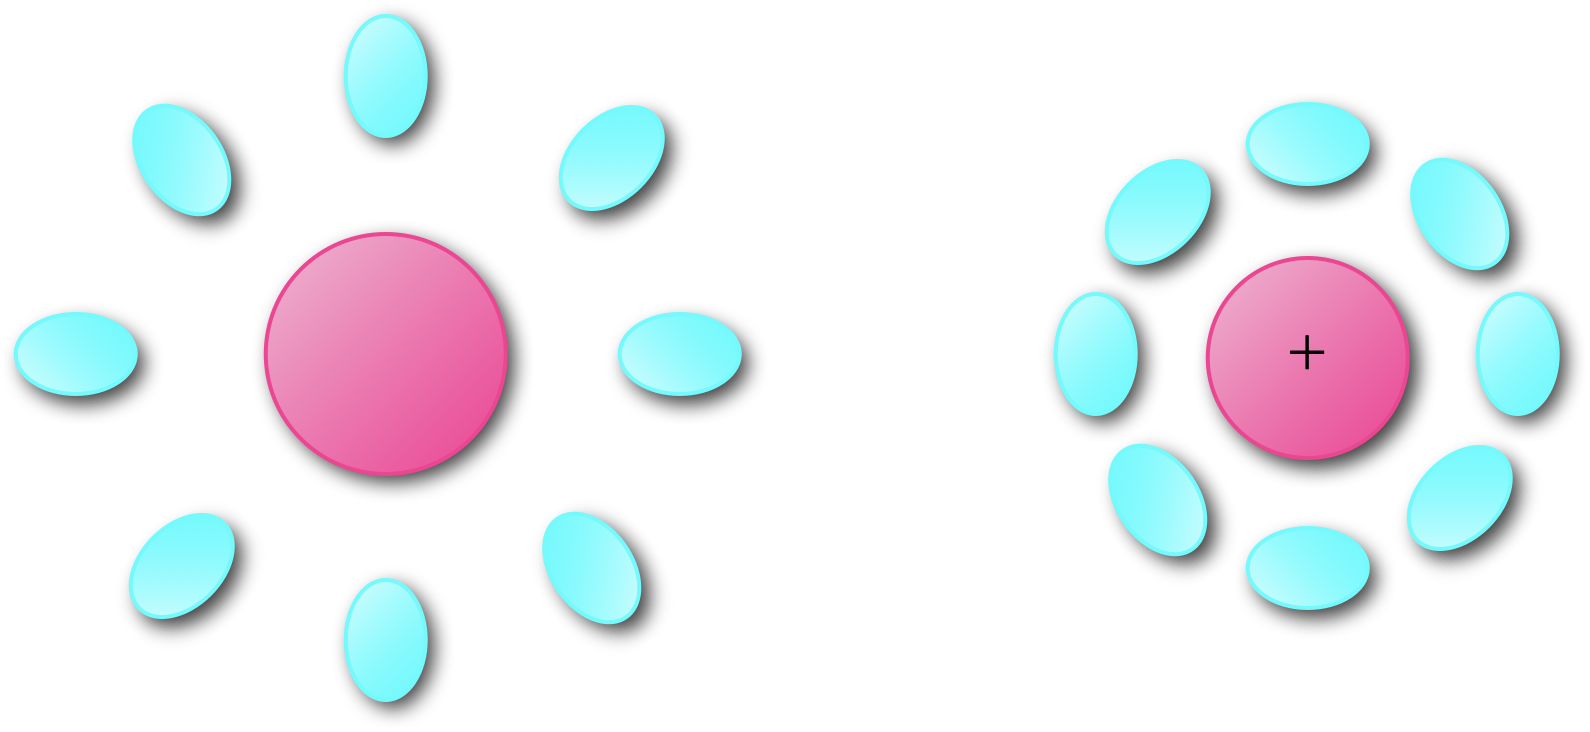
\includegraphics[width=0.5\linewidth]{images/elecreorg} 

}

\caption{Upon oxidation there is a reorganisation of both the molecule and its surrounding environment to minimize the energy of the structure.}\label{fig:elecreorg}
\end{figure}

This electron transfer is essentially instantaneous, and using the same justification as was used when considering the Franck-Condon principle, upon transfer of an electron from a donor to an acceptor the product of the electron transfer between the two molecules initially has the same structure. This excited state then relaxes within a few picoseconds to optimise the states of the products, figure \ref{fig:electransreorg}.

\begin{figure}

{\centering 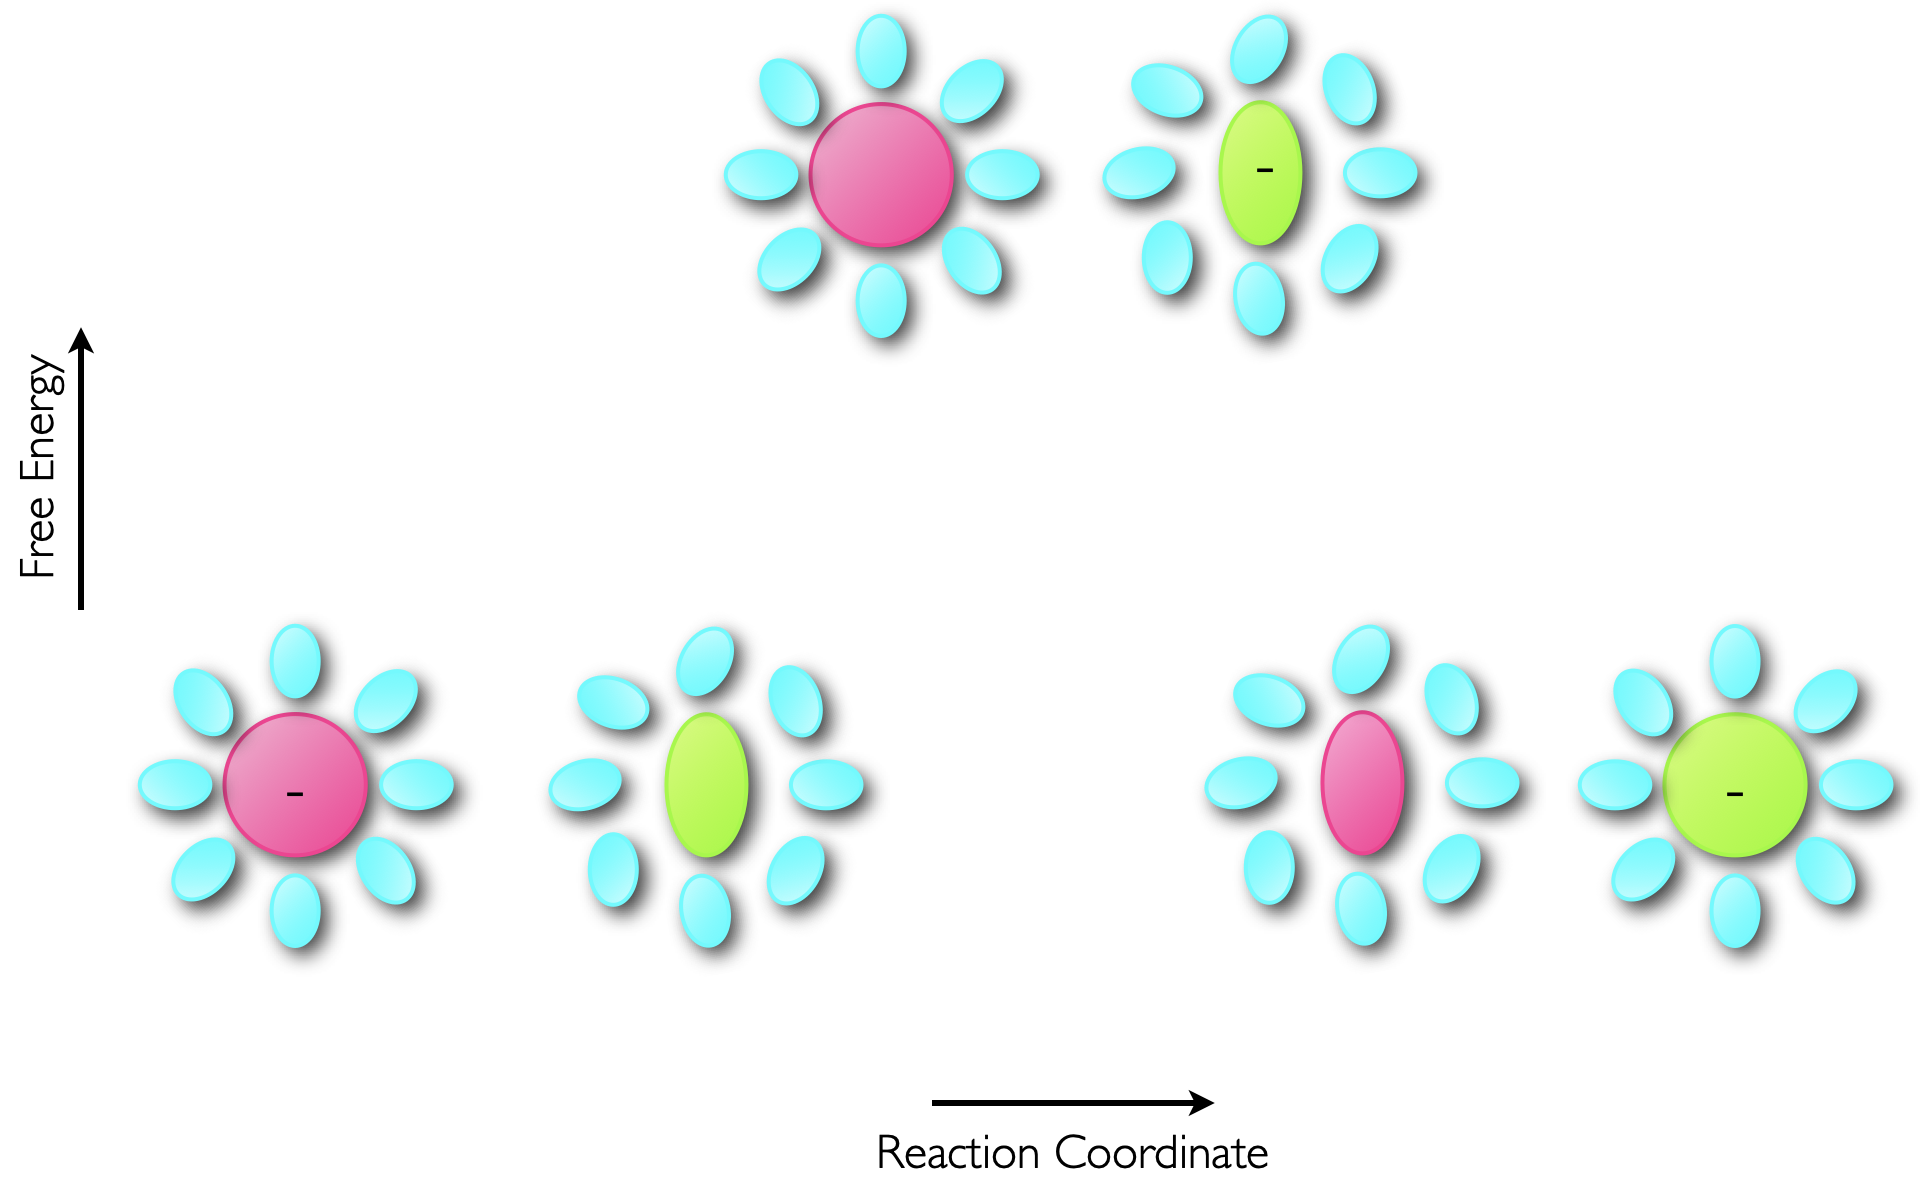
\includegraphics[width=0.6\linewidth]{images/electransreorg} 

}

\caption{The transfer of an electron from a donor to acceptor occurs within a few femtoseconds, which is considerably faster than molecular vibrations (which occur on the ps timescale) so the electron transfer results in an excited state product which then reorganises to minimise the energy of the product.}\label{fig:electransreorg}
\end{figure}

This energy is called the reorganisation energy, and appears with the symbol \(\lambda\) in equation \eqref{eq:marcus}. This reorganisation energy can be visualised by the vertical transition from the bottom of the potential energy well of our reactants to the potential energy well of the products, figure \ref{fig:reorgen}.

\begin{figure}

{\centering 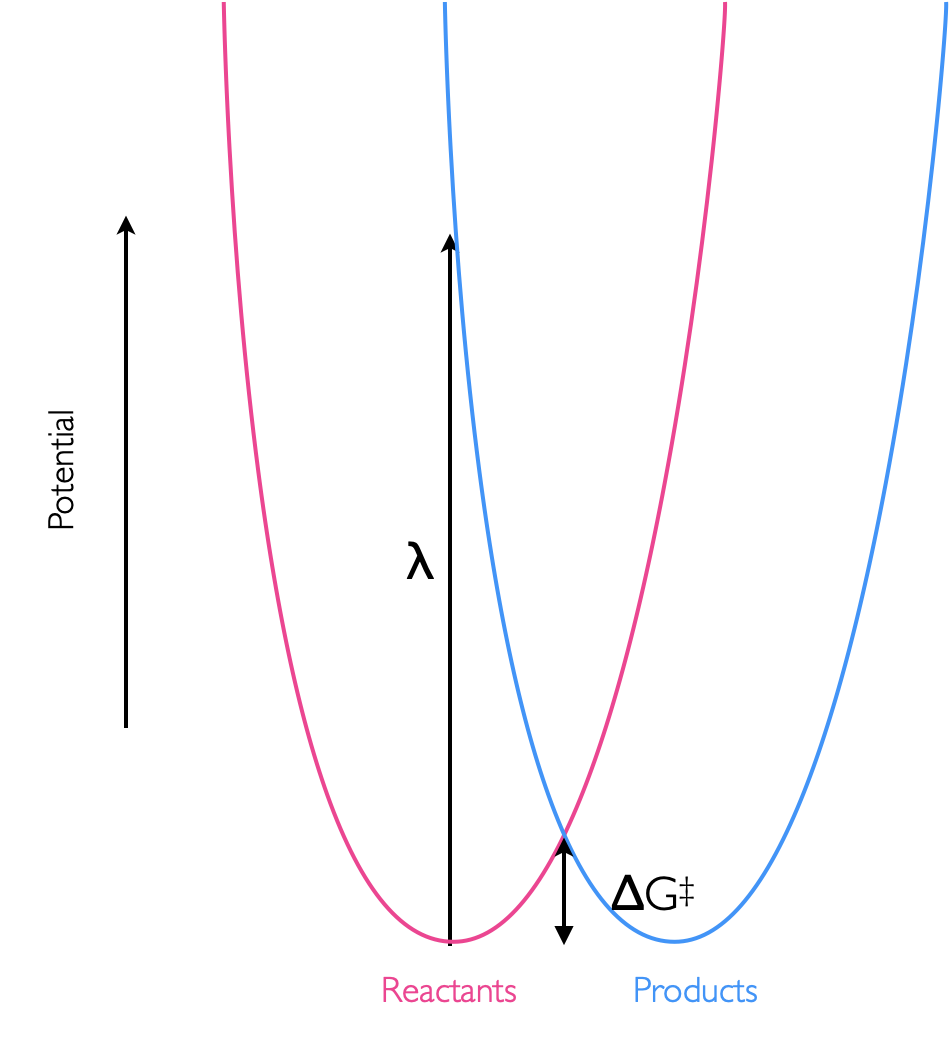
\includegraphics[width=0.4\linewidth]{images/reorgen} 

}

\caption{The reorganisation energy, λ, of an isoenergetic reaction, is the energy of the vertical transition between the potential wells of hte reactants and products. This reorganisation energy in this case is considerably higher than the activation energy of the reaction, ΔG‡}\label{fig:reorgen}
\end{figure}

The final, as yet undiscussed term in the marcus equation (equations \eqref{eq:marcus} \& \eqref{eq:coupel}) is the electronic coupling element \(|V(r)|\), this like the `overlap integral' from before is a measure of the overlap of the molecular orbitals, but this time of the two states (reactant \& product) of the donor and acceptor.

This value has a maximum at the van der Waals separation (\(r_o\) = 3.4 Å), and decreases exponentially with distance (\(r\)) (figure \ref{fig:distdepend}). The term \(\beta\) is a distance dependence scaling factor which describes how well the medium couples the donor and acceptor wavefunctions.

\begin{figure}

{\centering 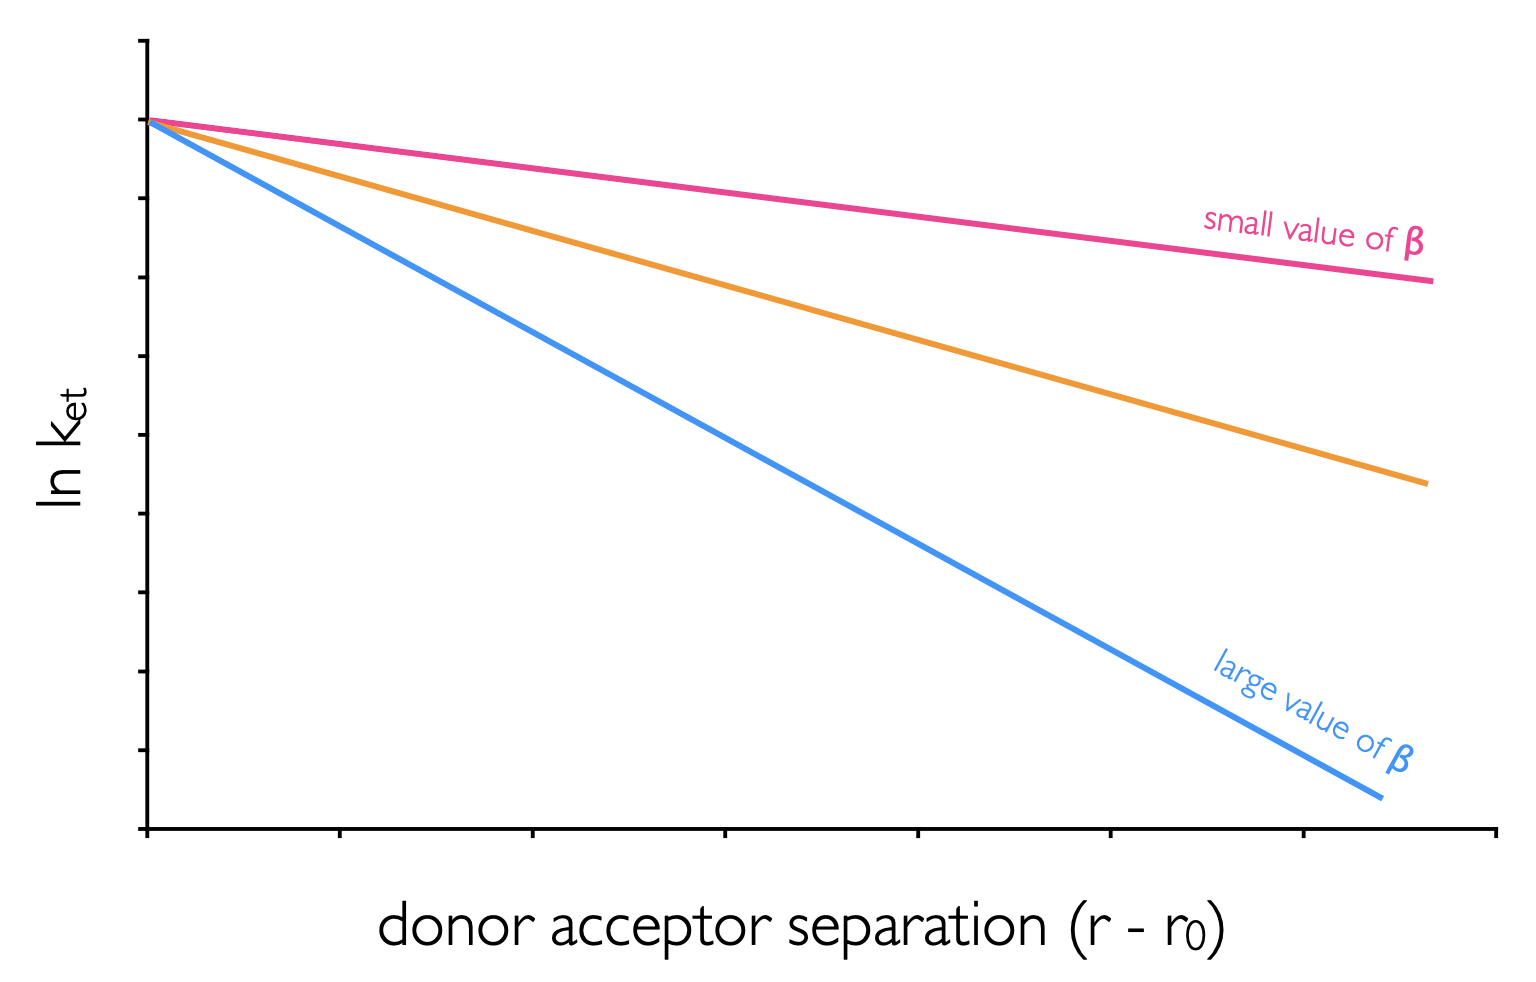
\includegraphics[width=0.6\linewidth]{images/distdepend} 

}

\caption{The distance dependence of electron transfer between donor and acceptor in mediums with different values of the distance dependence scaling factor, β. }\label{fig:distdepend}
\end{figure}

Figure \ref{fig:reorgen} shows an isoenergetic reaction, where the driving force of the reaction, \(\Delta G^\circ=0\). The transition state energy (the energy of the activation barrier) is related to the reorganisation energy, \(\lambda\) with the relationship shown in equation \eqref{eq:transstate}.

\begin{equation}
\Delta G^\ddagger_{\textrm{et}}=\frac{(\Delta G^\circ_{\textrm{et}}+ \lambda)^2}{4\lambda}
\label{eq:transstate}
\end{equation}

This gives two special cases, for the isoenergetic reaction where \(\Delta G^\circ=0\) the activation barrier \(\Delta G^\ddagger=\frac{\lambda}{4}\). Then for the case where the driving force of the reaction, \(\Delta G^\circ=\lambda\), then the activation barrier \(\Delta G^\ddagger=0\), and there is no barrier to the reaction occuring, figure \ref{fig:marcus}.

\begin{figure}

{\centering \includegraphics[width=1\linewidth]{images/marcus} 

}

\caption{The electron transfer between donor and acceptor with differing driving forces ΔGº, the potential energy wells of reactants (pink) and products (blue), with the reorganisation being the vertical transition from the bottom of the reactant well, and the activation energy, ΔG‡, being that from the bottom of the reactant potential well to the point where the two potential wells cross.}\label{fig:marcus}
\end{figure}

This leads to an interesting effect, as the driving force of a reaction increases the rate also increases until the point where the driving force and the reorganisation energy are the same. After this point the rate of reaction slows down, and this is perhaps an unusual and unexpected result. However, reaching this `Marcus inverted region', which typically requires a driving force of around -250 kJ mol\textsuperscript{-1}, is diffiuclt, and only photochemical (or electrochemical) reactions, where additional energy is provided to increase the driving force have so far been found to reach this Marcus inverted region, \ref{fig:marcusinverted}.

\begin{figure}

{\centering \includegraphics[width=0.5\linewidth]{images/marcusinverted} 

}

\caption{The rate of reaction increases with increasing driving force to a maximum where -ΔGº = λ, where the rate of reaction reaches a maximum. As the driving force of reaction increases teh rate of electron transfer slows down due to increasing solvent and molecular reorganization effects, this is called the Marcus inverted region. This effect is attenuated if the reaction is diffusion controlled as the rate of diffusion is often slower than the maximum possible rate of electron transfer.}\label{fig:marcusinverted}
\end{figure}

If the reactants in the donor acceptor electron transfer system are not held in rigid structure they then may diffuse together. This may ameliorate the possible rate of electron transfer (k\_\textrm{obs})as the observed rate of reaction is attenuated by diffusion effects (with rate \(k_\textrm{d}\))as described in equation (\eqref{eq:kobs}).

\begin{equation}
k_\textrm{obs}= \frac{k_\textrm{et}k_\textrm{d}}{k_\textrm{et}+k_\textrm{d}}
\label{eq:kobs}
\end{equation}

To observe the Marcus inverted region working in rigid or viscous solvent where diffusion is limited is one possibility, or else using a rigid scaffold to hold rigidly the donor and acceptor is also another way to observe this phenomenon. However, the Marcus inverted region is infact mostly likely to be observed in charge recombination reactions\footnote{There are a number of papers which show the Marcus}.

\hypertarget{sec:ETinDNA}{%
\section{Electron transfer reactions in DNA}\label{sec:ETinDNA}}

The assymetric cyanine dye YO-Pro-1 has been shown to fluoresce when bound to DNA, but further this fluorescence decreases over time. This decrease in fluorescence has been shown to be due to one electron oxidation of the modified base 7,8-dihydro-8-oxodeoxyguanosine (8-oxoG) reducing the chromophore and quenching the excited state. The reaction was studied by both steady state and time resolved fluorescence techniques (figure \ref{fig:YOquench} and table \ref{tab:YOquench}).

\begin{figure}

{\centering \includegraphics[width=0.7\linewidth]{images/YOquench} 

}

\caption{The measured normalised steady state fluorescence of YO-Pro-1 when bound to a 15mer oligonucleotide of DNA. The sequence of DNA variously had no modified bases, one 8-oxoG, or four 8-oxoG lesions.}\label{fig:YOquench}
\end{figure}

\begin{longtable}[]{@{}llll@{}}
\caption{\label{tab:YOquench} The normalised fluorescence intensity at λ\_max\_ and the lifetimes and normlised lifetimes for YO-Pro-1 when bound to a 15-mer oligonucleotide containing a varying number of modified lesions. The concentration of YO-Pro-1 was such that statistically there was no more than one dye bound per oligonucleotide.}\tabularnewline
\toprule
& Normalised Fluorescence & \(\tau\) / ns & \(\tau / \tau_0\) \\
\midrule
\endfirsthead
\toprule
& Normalised Fluorescence & \(\tau\) / ns & \(\tau / \tau_0\) \\
\midrule
\endhead
no modified bases & 1 & 2.80 & 1 \\
1 8-oxo-G & 0.558 & 2.38 & 0.85 \\
4 8-oxo-G & 0.169 & 1.31 & 0.47 \\
\bottomrule
\end{longtable}

You will recall that in Section @ref(\{sec:ratesphoto\}) the lifetime and quantum yield of a process were introduce, and it was stated that the ratios of both the lifetime and fluorescence intensity of the quenched to unquenched systems should be the same, however it is clear from the values in Table @ref\{tab:YOquench\} that this is not the case.

However, the lifetimes listed are actually multicomponent (there are multiple first order exponential decays overlayed), of which the instrument used could only measure longer lifetimes (\textgreater{} 0.8 ns). If the system is instead modeled as being a ladder with the modified base and dye held rigidly in one of a number of distance separations then the `calculated normlalised average lifetime' and the normalised fluorescence take the same values.

This case has been mentioned here to highlight limitations of measured lifetimes where the instrument used has to be suitable for the lifetimes you are measuring. It also highlights that Marcus theory is useful even if we are not interested in the Marcus inverted region.

If you wish to learn more about systems where there is more than one component in the emission, and what this means the unit CH40227 discusses such systems.

\hypertarget{sec:photosyn}{%
\section{Photosynthesis}\label{sec:photosyn}}

Photosynthesis is a photosensitised redox process whereby plants and some micro organisms convert carbon dioxide to carbohydrates and other organic molecules. The general reaction scheme is:

\begin{equation}
\textrm{nCO}_2+ \textrm{nH}_2\textrm{O} + h \nu \longrightarrow \textrm{(CH}_2 \textrm{O)}_\textrm{n}+ \textrm{nO}_2
\label{eq:photosyn}
\end{equation}

at standard temperatures this reaction is very exergonic (ΔG \textasciitilde{} +500 kJ mol\textsuperscript{−1}), and the chemistry involved in the process is very complicated but some key concepts are described here.

Principally it is a 4 electron process, the two half reactions are:

\begin{equation}
2\textrm{H}_2\textrm{O} \longrightarrow \textrm{O}_2 + 4\textrm{H}^+ + 4\textrm{e}^-
\label{eq:photosynhalf1}
\end{equation}

\begin{equation}
\textrm{CO}_2+ 4\textrm{H}^+ + 4\textrm{e}^- \longrightarrow \textrm{(CH}_2 \textrm{O)}^+ + \textrm{H}_2\textrm{O}
\label{eq:photosynhalf2}
\end{equation}

There are a number of different steps in photosynthesis, which can be broken down into two classes of reaction. Light reactions (reactions requiring the input of a photon) involve the production of oxygen and dark reactions (reactions not requiring a photon) use the electrons and protons gained from the light reactions in order to reduce the carbon dioxide.

In order to harvest light for the reactions plants have a number of pigments, which cover a broad range of the visible spectrum. The pigment chlorophyl consists of a porphyrin ring ligated to a magnesium centre. In addition to chlorophyl plants have other conjugated molecules in order to harvest other wavelengths of light. These carotenoids principally absorb blue and green light which then transfers to the reaction centre, however these carotenoids also act as quenching agents in order to `hoover up' any stray oxidising agents (principally singlet oxygen).

Charge separation in photosynthesis is incredibly important process, and is perhaps the most difficult step to replicate in artificial photosynthetic systems. There are also difficulties large structural changes and the large driving force required in order to replicate photosynthesis. Nature uses two reaction centres and harvests light from other antenna modules and currently artificial systems have no where near this complexity, however this is a leading topic of research and a number of different systems, either inspired by or totally removed from nature are currently being developed.

This has been an introduction to photosynthesis, but you should now read pages 222-232 or Wardle.

\hypertarget{sec:PDT}{%
\section{Photodynamic Therapy}\label{sec:PDT}}

Current research in photochemistry isn't solely interested in light harvesting; there is also a large interest in using light in medicine. The most obvious biological use of light is in the essential production of vitamin D, however there are a number of unwanted photoactive reactions that occur, since both DNA and proteins may absorb UV light.

\begin{figure}

{\centering \includegraphics[width=0.5\linewidth]{images/DNAbases} 

}

\caption{The base pairs in DNA, the purines guanosine and adenosine hydrogen bond to the pyrimidine bases cytosine and thymidine respectively. Conjugation in the bases means they all have good absorptions of around 6600 M−1 cm−1 at 260 nm.}\label{fig:DNAbases}
\end{figure}

DNA undergoes a range of photochemical reactions, depending on the excitation wavelength, with either pyrimidine dimers (figure \ref{fig:Tdimer}) or one electron oxidation of guanine forming the lesion 8-oxo-guanine being the principle products. Both of these adducts lead to mutations when replicating DNA, although there are a number of repair pathways mutations are inevitable. The pyrimidine dimerisation is particularly efficient as the reactants are already held closely together in the DNA structure.

There has been a great deal of interest in the field of phototheraputics; or using light in a medicinal context. The molecule methylene blue has been used for a number of years a sterilising agent as it is an efficient sensitiser of singlet oxygen, the blue colour is indicative of absorption of red wavelengths of light which makes it useful therapeutically as blood transmits red light. In fact methylene blue has undergone field trials for photosterilisation of blood products in remote areas. The concept being blood products need all DNA removed, wether pathogens or donor white blood cells, methylene blue is indiscriminate in the photosensitised oxidative reactions and any easily oxidisable reactant is damaged.

\begin{figure}

{\centering \includegraphics[width=0.4\linewidth]{images/Tdimer} 

}

\caption{The structure of a thymidine dimer adduct formed by absorption of UV light.}\label{fig:Tdimer}
\end{figure}

Using a slightly more targeted approach a number of molecules have been developed for use in photodynamic therapy for treatment of conditions such as cancer. Traditional chemotherapies make use of the higher metabolic rate of cancerous cells and a generally not very specific, which is the reason for the large number of side effects. Photodynamic therapy hopes to use a drug which is completely non toxic in the `dark state' but upon absorption of a photon the molecule becomes highly reactive to either DNA or proteins. Since light can be easily directed only the treated area is generates toxins, however this means that only accessible regions such skin and lungs may be treated. An ideal photodynamic agent will be blue (have a red absorption) so that the light may be transmitted through the skin and blood vessels and will be highly active. Cells have a number of `anti oxidant' repair mechanisms and so damage has to be significant so as to either stop cell replication or cause apoptosis.

\hypertarget{before-completing-this-section-3}{%
\section{Before Completing this Section}\label{before-completing-this-section-3}}

To support the material in this section it is suggested you read chapters 8 \& 12 of Wardle `Principles and Application of Photochemistry'.

  \bibliography{book.bib,packages.bib}

\end{document}
